% ============================================================================
% DOCUMENTO PRINCIPAL - Tesis de Ingeniería de Sistemas
% Universidad Nacional del Altiplano - Puno
% ============================================================================

% Cargar preámbulo
% ============================================================================
% PREÁMBULO - Configuraciones y Paquetes (Alineado a Guía UNAP 2.0 y APA 7)
% ============================================================================

% Clase de documento
\documentclass[12pt,oneside]{book}

% -------------------------------------------------------------------------
% Paquetes fundamentales y Tipografía
% -------------------------------------------------------------------------

% Idioma español - Traducir "Cuadro" como "Tabla"
\usepackage[spanish,es-tabla]{babel}
\addto\captionsspanish{\def\tablename{Tabla}}

% Codificación UTF-8
\usepackage[utf8]{inputenc}

% Paquete para geometría de páginas (Márgenes UNAP)
\usepackage{geometry}

% Paquete para sangría francesa en bibliografía APA 7
\usepackage{hanging}

% Paquete para ecuaciones matemáticas básicas
\usepackage{amsmath}
\usepackage{amssymb}
\usepackage{amsfonts}
\usepackage{bm}

% Paquetes para diagramas, esquemas y tablas anchas
\usepackage{tikz}
\usetikzlibrary{shapes.geometric, arrows, positioning, fit, calc, backgrounds, babel}
\usepackage{pgfplots}
\pgfplotsset{compat=1.18}
\usepackage{pdflscape}

% Fuente Times New Roman (12pt según Guía UNAP)
\usepackage{mathptmx}

% Interlineado 1.5 (Configurado según estándar UNAP)
\usepackage{setspace}
\setstretch{1.5}

% Márgenes Oficiales UNAP:
% Izquierdo: 3.0 cm (para empastado)
% Derecho: 2.5 cm | Superior: 2.5 cm | Inferior: 2.5 cm
\geometry{
    left=3.0cm,
    right=2.5cm,
    top=2.5cm,
    bottom=2.5cm
}

% -------------------------------------------------------------------------
% Control de Párrafos y Formato
% -------------------------------------------------------------------------

% Control de líneas huérfanas/viudas
\widowpenalty=10000
\clubpenalty=10000

% Sangría de primera línea (1.25 cm según APA 7 / Guía UNAP)
\usepackage{indentfirst}
\setlength{\parindent}{1.25cm}

% Saltos de página controlados
\usepackage{emptypage}

% Formato de encabezados y pies de página (Numeración en pie de página centrado)
\usepackage{fancyhdr}
\fancyhf{}
\fancyhead[C]{}
\fancyfoot[C]{\thepage}
\pagestyle{fancy}
\renewcommand{\headrulewidth}{0pt}

% Hipervínculos en el PDF
\usepackage{url}
\usepackage[colorlinks=true,linkcolor=black,anchorcolor=black,citecolor=black,filecolor=black,urlcolor=black]{hyperref}

% -------------------------------------------------------------------------
% Configuración de Tablas y Figuras (Guía UNAP 2.0 / APA 7)
% -------------------------------------------------------------------------

\usepackage{graphicx}
\graphicspath{{figuras/}}

\usepackage{float}
\usepackage{array}
\usepackage{tabularx}
\usepackage{booktabs}
\usepackage{caption}

% Estilo de Leyendas (Captions) alineado a Guía UNAP págs. 21 y 22:
% "Tabla 1" en Negrita, Salto de línea, y Título descriptivo en Cursiva
\DeclareCaptionFormat{unap}{\textbf{#1}\\\textit{#3}}
\captionsetup{
    format=unap,
    justification=raggedright,
    singlelinecheck=false,
    labelfont=bf,
    font=normalsize,
    skip=5pt
}

% -------------------------------------------------------------------------
% Configuración de Títulos y Capítulos (Guía UNAP 2.0)
% -------------------------------------------------------------------------

\usepackage{titlesec}

% CAPÍTULO I (16pt, Negrita, Centrado)
% TÍTULO DEL CAPÍTULO (14pt, Negrita, Centrado, MAYÚSCULA)
\titleformat{\chapter}[display]
    {\bfseries\centering}
    {\Large\MakeUppercase{CAPÍTULO \Roman{chapter}}}
    {5pt}
    {\large\MakeUppercase}
    []

\titlespacing*{\chapter}{0pt}{-10pt}{20pt}

% NIVEL 2 (Ej. 1.1. TÍTULO SECCIÓN) - MAYÚSCULA, Negrita, Izquierda
\titleformat{\section}
    {\bfseries\normalsize\raggedright}
    {\thesection}
    {0.5em}
    {\MakeUppercase}

% Configuración de profundidad de numeración y tabla de contenidos (Nivel 4: 2.2.1.1)
\setcounter{secnumdepth}{3}
\setcounter{tocdepth}{3}

% NIVEL 3 (Ej. 2.2.1. Título Subsección) - Minúscula, Negrita, Izquierda
\titleformat{\subsection}
    {\bfseries\normalsize\raggedright}
    {\thesubsection}
    {0.5em}
    {}

% NIVEL 4 (Ej. 2.2.1.1. Título Sub-subsección) - Minúscula, Negrita, Izquierda
\titleformat{\subsubsection}
    {\bfseries\normalsize\raggedright}
    {\thesubsubsection}
    {0.5em}
    {}

% -------------------------------------------------------------------------
% Listas y Viñetas
% -------------------------------------------------------------------------
\usepackage{enumitem}
\setlist[itemize]{leftmargin=1.25cm, topsep=2pt, itemsep=2pt}
\setlist[enumerate]{leftmargin=1.25cm, topsep=2pt, itemsep=2pt}

% Inicio del documento
\begin{document}

% ----- PÁGINAS PRELIMINARES -----
\pagenumbering{arabic}

% Portada
\thispagestyle{empty}
\begin{titlepage}

\thispagestyle{empty}

% Bloque 1: Institución
\begin{center}
    \Large\textbf{UNIVERSIDAD NACIONAL DEL ALTIPLANO - PUNO}
    \vspace{0.5cm}

    \Large\textbf{FACULTAD DE INGENIERÍA MECÁNICA ELÉCTRICA, ELECTRÓNICA Y SISTEMAS}
    \vspace{0.5cm}

    \Large\textbf{ESCUELA PROFESIONAL DE INGENIERÍA DE SISTEMAS}
\end{center}

% Bloque 2: Logo institucional
\begin{center}
    
\includegraphics[width=5cm]{figuras/Logo_UNAP.png}
\end{center}

% Bloque 3: Título de la Tesis
\begin{center}
    \Large\textbf{DETECCIÓN DE ATAQUES MINORITARIOS EN REDES IoT MEDIANTE UN MODELO HÍBRIDO BASADO EN STACKING, XGBOOST Y LIGHTGBM, PUNO 2026}
\end{center}

% Bloque 4: Motivo
\begin{center}
    \normalsize BORRADER DE TESIS

    \normalsize PRESENTADA POR:
\end{center}

% Bloque 5: Autor
\begin{center}
    \large\textbf{CARMEN NIEVES APAZA CONDORI}
\end{center}

% Bloque 6: Grado
\begin{center}
    \normalsize PARA OPTAR EL TÍTULO PROFESIONAL DE: \\[0.3cm]
    \large\textbf{INGENIERO DE SISTEMAS}
\end{center}

% Bloque 7: Lugar y Fecha
\vfill

\begin{center}
    PUNO - PERÚ

    2026
\end{center}

\end{titlepage}

% Hoja de aprobación de jurados
\thispagestyle{plain}
\input{jurados}

% Índice General (Tabla de contenidos)
\thispagestyle{plain}
\tableofcontents
\addcontentsline{toc}{chapter}{Índice General}

% Índice de tablas
\thispagestyle{plain}
\listoftables
\addcontentsline{toc}{chapter}{Índice de Tablas}

% Índice de figuras
\thispagestyle{plain}
\listoffigures
\addcontentsline{toc}{chapter}{Índice de Figuras}

% Índice de acrónimos
\input{capitulos/acronimos}

% Resumen y Abstract
\chapter*{RESUMEN}
\addcontentsline{toc}{chapter}{Resumen}
\markboth{RESUMEN}{RESUMEN}

El constante crecimiento del Internet de las Cosas (IoT) en las empresas enfrenta graves vulnerabilidades, ya que los Sistemas de Detección de Intrusiones (IDS) tradicionales tienen muy poca sensibilidad para detectar ciberataques que son infrecuentes pero sumamente peligrosos, como aquellos basados en web o de fuerza bruta. Para solucionar esto, esta investigación desarrolló y evaluó un modelo híbrido de clasificación apoyado en una arquitectura Stacking de dos niveles, combinando los algoritmos Random Forest, XGBoost GPU y LightGBM. Todo esto fue reforzado con la Entropía de Shannon para medir la incertidumbre y la técnica Borderline-SMOTE1 para equilibrar los datos. Este diseño cuasi-experimental se aplicó sobre el dataset CICIoT2023, analizando más de 2.5 millones de flujos de red totalmente limpios, destinando el 80\% de la información para el entrenamiento y aislando el 20\% exclusivamente para las pruebas. Los resultados demostraron el éxito de la propuesta al lograr un F1-Macro del 70.18\% y una exactitud del 84.85\%, superando con claridad a todos los modelos individuales evaluados. Además, registró un desempeño asombroso con una latencia de apenas $8.65\,\mu s$ por flujo y un consumo mínimo de $257.89\text{ MB}$ de memoria RAM, garantizando que puede funcionar sin problemas en pasarelas de borde. Finalmente, tras confirmar su validez matemática mediante la Prueba de Wilcoxon ($p = 0.003744 < 0.05$), concluimos con certeza que mezclar estos clasificadores resulta ser una solución sumamente eficaz, rápida y liviana para proteger las redes IoT.

\vspace{0.5cm}
\noindent \textbf{Palabras clave:} Ataques minoritarios, Borderline-SMOTE, CICIoT2023, Ciberseguridad, Entropía de Shannon, Internet de las Cosas, Stacking híbrido.

\clearpage
\chapter*{ABSTRACT}
\addcontentsline{toc}{chapter}{Abstract}
\markboth{ABSTRACT}{ABSTRACT}

The constant growth of the Internet of Things (IoT) in businesses faces serious vulnerabilities, as traditional Intrusion Detection Systems (IDS) have very low sensitivity when it comes to detecting cyberattacks that are infrequent but highly dangerous, such as web-based or brute force attacks. To address this issue, this research developed and evaluated a hybrid classification model based on a two-level Stacking architecture, combining the Random Forest, XGBoost GPU, and LightGBM algorithms. This approach was reinforced with Shannon Entropy to measure uncertainty and the Borderline-SMOTE1 technique to balance the data. This quasi-experimental design was applied to the CICIoT2023 dataset, analyzing over 2.5 million fully cleansed network flows, strategically allocating 80\% of the information for training and isolating the remaining 20\% exclusively for testing. The results demonstrated the success of the proposal by achieving an F1-Macro of 70.18\% and an accuracy of 84.85\%, clearly outperforming all the individual models evaluated. Furthermore, it recorded an astonishing computational performance with a latency of just $8.65\,\mu s$ per flow and a minimal consumption of 257.89 MB of RAM, ensuring it can operate smoothly on edge gateways. Finally, after confirming its mathematical validity through the Wilcoxon Test ($p = 0.003744 < 0.05$), we can conclude with absolute certainty that combining these classifiers provides a highly effective, fast, and lightweight solution for protecting IoT networks.

\vspace{0.5cm}
\noindent \textbf{Keywords:} Borderline-SMOTE, CICIoT2023, Cybersecurity, Hybrid Stacking, Internet of Things, Minority Attacks, Shannon Entropy.


% ----- CONTENIDO PRINCIPAL -----
\clearpage
\pagenumbering{arabic}

% Capítulo I: Introducción
\chapter{INTRODUCCIÓN}

\section{CONTEXTUALIZACIÓN}

La instalación masiva de dispositivos interconectados a través del famoso Internet de las Cosas (IoT) ha logrado transformar por completo nuestra infraestructura digital a nivel global, haciendo muchísimo más fácil la automatización en áreas tan críticas como la industria 4.0, el manejo de ciudades inteligentes, la telemedicina y el monitoreo del medio ambiente, pero lamentablemente toda esta rápida expansión también ha traído consigo un enorme problema al aumentar de forma explosiva nuestro nivel de exposición ante ciberataques que resultan ser cada vez más complejos y destructivos, una situación que se vuelve todavía más complicada de manejar si tomamos en cuenta que las redes IoT son sumamente variadas y que la gran mayoría de estos pequeños equipos sufren de fuertes limitaciones físicas en cuanto a su memoria, batería y capacidad de procesamiento, lo cual provoca que sea prácticamente imposible intentar protegerlos instalándoles los típicos sistemas de seguridad tradicionales como los cortafuegos pesados o las herramientas de inspección profunda de datos (Sama et al., 2025).

A pesar de que los Sistemas de Detección de Intrusiones (IDS) basados en aprendizaje automático han avanzado muchísimo, la realidad es que al momento de identificar anomalías en entornos de red reales se topan de frente con un enorme desafío técnico conocido como el desbalance extremo de clases, una situación que ocurre porque en el día a día la inmensa cantidad de tráfico normal junto con los ataques masivos de denegación de servicio (DDoS) terminan inundando por completo los registros, provocando que los ciberataques mucho más sofisticados y silenciosos, como las inyecciones Web, los desbordamientos de búfer o los ataques de fuerza bruta, sucedan con una frecuencia tan baja que casi quedan sepultados (Ahmed et al., 2024), lo cual lamentablemente genera un fuerte sesgo algorítmico en los clasificadores convencionales, quienes terminan engañándose a sí mismos al tratar de optimizar su exactitud global a costa de ignorar casi por completo a estas muestras minoritarias que, irónicamente, son las que terminan representando las brechas de seguridad más disruptivas y peligrosas para todo el sistema.

Para tratar de mitigar esta gran vulnerabilidad, la comunidad científica ha comenzado a explorar nuevas alternativas como las arquitecturas de aprendizaje jerárquico, también conocidas como Stacking, aunque rápidamente se dieron cuenta de que simplemente mezclar varios clasificadores no es suficiente si no se le añaden mecanismos matemáticos capaces de medir la incertidumbre que se genera en esas zonas donde los datos están tan desbalanceados, por lo que integrar herramientas como la Entropía de Shannon ha resultado ser un paso clave para lograr evaluar qué tan confundidos están los modelos base, algo que, al combinarse con técnicas mucho más avanzadas para equilibrar los datos en la frontera como lo es el Borderline-SMOTE, nos permite devolverle su verdadera importancia a esos ataques menos frecuentes sin terminar ensuciando el sistema con información sintética perjudicial (Popoola et al., 2025; Nigar \& Mustafa, 2025), abriendo así la puerta para construir un gran modelo híbrido donde la poderosa sinergia entre Random Forest, XGBoost y LightGBM, trabajando todos bajo la supervisión de un meta-clasificador superior, nos ofrezca por fin una solución que no solo es capaz de adaptarse de maravilla a diferentes situaciones, sino que además cuenta con una velocidad de respuesta increíblemente rápida y ultrabaja, haciéndola ideal para proteger los complejos entornos de las redes IoT.

\section{REALIDAD PROBLEMÁTICA}

Si miramos el panorama a nivel internacional, nos damos cuenta de que la adopción masiva de tecnologías del Internet de las Cosas (IoT) tanto en la industria como en el comercio ha terminado exponiendo a las organizaciones a un número cada vez mayor de amenazas cibernéticas, una cruda realidad que golpea especialmente a las pequeñas y medianas empresas (PYMEs) de todo el mundo, quienes enfrentan un desafío gigantesco para proteger sus entornos digitales simplemente porque carecen de sistemas de ciberseguridad que se ajusten a su verdadera capacidad tecnológica (Ciampi et al., 2021), y aunque es cierto que el aprendizaje automático nos ofrece alternativas muy prometedoras para detectar estas intrusiones, el gran problema es que la mayoría de las soluciones actuales fracasan rotundamente cuando tienen que lidiar con conjuntos de datos que están altamente desbalanceados, tal como ocurre con el famoso referente internacional CICIoT2023, donde lamentablemente los ataques más sigilosos y destructivos, como aquellos basados en la web o los de fuerza bruta, apenas logran representar menos del 1\% de todo el tráfico, provocando que pasen totalmente desapercibidos y sean ignorados por los clasificadores convencionales (Nigar \& Mustafa, 2025).

Si aterrizamos esta problemática a nivel nacional, nos encontramos con que en el Perú las micro, pequeñas y medianas empresas (MYPEs y PYMEs) son el verdadero motor de la economía, ya que representan más del 98\% de todo nuestro tejido productivo y juegan un papel absolutamente fundamental en la generación de empleo para el país. Sin embargo, esta rápida carrera hacia la digitalización y la constante incorporación de dispositivos IoT en los negocios locales se está llevando a cabo bajo un escenario de altísima vulnerabilidad cibernética, una situación que se agrava enormemente debido a que estas empresas suelen operar con presupuestos muy limitados y sufren por la casi total ausencia de herramientas para detectar amenazas que estén verdaderamente adaptadas a nuestra propia realidad tecnológica (López-García et al., 2023). Toda esta preocupante realidad queda en evidencia al revisar la literatura nacional sobre el tema, donde estudios recientes aplicados sobre el dataset CICIoT2023, como los desarrollados por Raico Gallardo (2025), demuestran claramente que, si bien los clasificadores individuales logran detectar sin mucho esfuerzo el tráfico de ataques masivos, terminan fracasando de manera drástica cuando intentan identificar las intrusiones de baja frecuencia, un gran vacío que nos confirma la urgente necesidad de empezar a diseñar modelos integrados que por fin logren resolver problemas tan complejos como el rebalanceo de clases y el análisis de la incertidumbre para poder fortalecer de verdad la ciberseguridad a nivel nacional (Vargas-Hernández et al., 2022).

Si enfocamos nuestra mirada a nivel regional, específicamente en la región de Puno y en todo el sur del Perú, nos damos cuenta de que las pequeñas y medianas empresas dedicadas a la producción, el comercio y los servicios están viviendo una paulatina pero constante automatización a través del uso de sensores y dispositivos conectados. Sin embargo, todo este importante proceso de modernización se está llevando a cabo enfrentando grandes limitaciones en la infraestructura de red y operando con recursos computacionales bastante reducidos (Quispe-Mamani et al., 2023), un escenario que nos hace ver la urgencia de empezar a implementar modelos de detección de intrusos que, al ser probados rigurosamente en un entorno de laboratorio, nos permitan evaluar de manera segura qué tan factibles y eficientes resultan estas soluciones para nuestra realidad técnica. Es justamente por esta razón que la presente investigación nace con el propósito de cubrir ese gran vacío, desarrollando un modelo híbrido altamente optimizado que logra integrar la técnica Borderline-SMOTE, la Entropía de Shannon y la arquitectura de Stacking de clasificadores dentro de un entorno de laboratorio, ofreciendo así una solución concreta que no solo nos permite elevar drásticamente la capacidad para detectar esos escurridizos ataques minoritarios, sino que además lo hace exigiendo un mínimo consumo de recursos para adaptarse a las verdaderas posibilidades tecnológicas de nuestra región.

\section{FORMULACIÓN DEL PROBLEMA}

\subsection{Problema General}
¿En qué medida el Modelo híbrido basado en Stacking, XGBoost y LightGBM mejora la eficacia en la detección de ataques minoritarios en redes IoT?

\subsection{Problemas Específicos}
\begin{itemize}
\item \textbf{PE1:} ¿En qué grado la técnica de rebalanceo Borderline-SMOTE incrementa la proporción de balance de la clase minoritaria en el dataset CICIoT2023 respecto al balance original?
\item \textbf{PE2:} ¿Cuál es la capacidad de detección del Modelo híbrido basado en Stacking, XGBoost y LightGBM en la identificación de ataques minoritarios evaluada mediante las métricas de evaluación Recall, F1-Score y Accuracy?
\item \textbf{PE3:} ¿Cuál es la eficiencia computacional del Modelo híbrido basado en Stacking, XGBoost y LightGBM propuesto en términos de tiempos de entrenamiento y latencia de inferencia frente a los modelos base Random Forest y XGBoost?
\end{itemize}

\section{JUSTIFICACIÓN}

\subsection{Justificación Técnica y Científica}
Desde el punto de vista técnico, esta investigación nace de la gran necesidad de superar las limitaciones que tienen los clasificadores individuales cuando se enfrentan a datos sumamente desbalanceados en las redes IoT, y aunque la literatura científica más reciente ya nos ha demostrado que utilizar enfoques de ensamble por Stacking resulta ser mucho mejor que usar modelos independientes para lograr una buena capacidad de generalización (Sama et al., 2025; Ahmed et al., 2024), nuestra propuesta busca dar un paso más allá para evolucionar el estado del arte al integrar la Entropía de Shannon como una medida cuantitativa real de la incertidumbre, colocándola directamente dentro del vector de meta-características (el cual está compuesto por 27 atributos que se dividen en 24 probabilidades de clase y 3 indicadores entrópicos), un detalle que resulta absolutamente clave porque le otorga al meta-modelo LightGBM la capacidad de tomar decisiones con muchísima más precisión justo en aquellas zonas donde suele generarse una mayor confusión, sumando a todo esto la aplicación estratégica de la técnica Borderline-SMOTE exclusivamente sobre el conjunto de entrenamiento para lograr fortalecer enormemente las fronteras de decisión de esas clases minoritarias tan vulnerables (como los ataques basados en Web y de fuerza bruta) sin caer en el temido error de la fuga de datos o data leakage, garantizando así que todo nuestro protocolo metodológico se mantenga completamente robusto y libre de sesgos.

\subsection{Justificación Económica y Operativa}
Si lo analizamos desde una perspectiva mucho más operativa y de laboratorio, resulta evidente que los entornos de prueba para redes IoT necesitan con urgencia validar soluciones que ofrezcan una altísima velocidad de respuesta consumiendo la menor cantidad de memoria posible, y aunque los famosos modelos basados en aprendizaje profundo (Deep Learning) son muy potentes, la cruda realidad es que exigen demasiados recursos físicos y tardan muchísimo en ejecutarse, por lo que el modelo propuesto en esta investigación logra marcar una verdadera diferencia al demostrar una eficiencia sobresaliente en estas condiciones de prueba, logrando alcanzar una latencia de inferencia de apenas $8.65\,\mu\text{s}$ por muestra (lo que equivale a procesar más de 115,000 paquetes por segundo) junto con un ligerísimo consumo de memoria RAM de tan solo $257.89\text{ MB}$, cifras contundentes que respaldan y fundamentan por completo su viabilidad técnica para poder ser implementado en el futuro sin ningún problema dentro de aquellos dispositivos que cuentan con recursos sumamente limitados.

\subsection{Justificación Social y Práctica}
En cuanto a su impacto y relevancia social, el verdadero valor de este trabajo radica en brindar evidencia tanto empírica como tecnológica que nos permita proteger a fondo la integridad y la privacidad de las redes de información que utilizan las MYPEs y PYMEs en nuestra región y en todo el país, sobre todo si tenemos en cuenta que cuando un ciberataque logra pasar desapercibido en los sistemas de estas pequeñas empresas, puede terminar provocando pérdidas económicas sumamente graves e incluso obligarlas a paralizar por completo todas sus actividades comerciales, por lo que haber logrado validar experimentalmente este modelo utilizando los 63 archivos oficiales del dataset \textbf{CICIoT2023} termina entregándole a toda la comunidad académica y técnica una herramienta de ciberseguridad verdaderamente proactiva, muy fácil de reproducir y, sobre todo, que exige un costo computacional sumamente bajo para operar de manera eficiente.

\section{OBJETIVOS}

\subsection{OBJETIVO GENERAL}
Determinar la eficacia del Modelo Híbrido basado en Stacking, XGBoost y LightGBM en la mejora de la detección de ataques minoritarios en redes IoT.

\subsection{OBJETIVOS ESPECÍFICOS}
\begin{itemize}
\item \textbf{OE1:} Evaluar la mejora en la proporción de balance de la clase minoritaria mediante la aplicación de la técnica de rebalanceo Borderline-SMOTE en el dataset CICIoT2023.
\item \textbf{OE2:} Determinar la capacidad de detección del Modelo Híbrido basado en Stacking, XGBoost y LightGBM en la identificación de ataques minoritarios utilizando las métricas de evaluación Recall, F1-Score y Accuracy.
\item \textbf{OE3:} Comparar la eficiencia computacional del modelo híbrido propuesto midiendo los tiempos de entrenamiento y latencia de inferencia frente a los modelos base Random Forest y XGBoost.
\end{itemize}

\section{HIPÓTESIS DE LA INVESTIGACIÓN}

\subsection{Hipótesis general}
El Modelo Híbrido basado en Stacking, XGBoost y LightGBM mejora significativamente la eficacia (Recall y F1-Score) en la detección de ataques minoritarios en redes IoT, superando el rendimiento de los modelos base en el dataset CICIoT2023.

\subsection{Hipótesis específicas}
\begin{itemize}
\item \textbf{HE1:} La técnica de rebalanceo Borderline-SMOTE incrementa significativamente la proporción de balance de la clase minoritaria en el dataset CICIoT2023, reduciendo el índice de desbalance y mejorando la distribución de datos en la frontera de decisión.
\item \textbf{HE2:} El Modelo Híbrido XGB-LGBM-Stacking con análisis de incertidumbre presenta una alta capacidad de detección de ataques minoritarios, evidenciando indicadores superiores en las métricas de Recall, F1-Score y Accuracy al ser validados estadísticamente mediante la prueba de rangos con signo de Wilcoxon.
\item \textbf{HE3:} El modelo híbrido propuesto optimiza la eficiencia computacional, logrando tiempos de entrenamiento y una latencia de inferencia competitivos en comparación con los modelos base Random Forest y XGBoost, garantizando su viabilidad operativa.
\end{itemize}

\section{VARIABLES}

\subsection{Variable Independiente (VI)}
Modelo híbrido basado en Stacking, XGBoost y LightGBM, optimizado con la técnica de rebalanceo de datos Borderline-SMOTE.

\subsection{Variable Dependiente (VD)}
Detección de ataques minoritarios en redes IoT, evaluada a través de la eficacia predictiva y el desempeño computacional.

\section{OPERACIONALIZACIÓN DE VARIABLES}

\begin{table}[H]
\centering
\caption{Matriz de Operacionalización de Variables de la Investigación}
\label{tab:operacionalizacion}
\small

\begin{tabularx}{\textwidth}{>{\raggedright\arraybackslash}p{2.2cm} >{\raggedright\arraybackslash}p{2.6cm} >{\raggedright\arraybackslash}p{2.6cm} >{\raggedright\arraybackslash}p{2.2cm} >{\raggedright\arraybackslash}p{2.8cm} >{\raggedright\arraybackslash}p{2.0cm}}
\toprule
\textbf{Variable} & \textbf{Definición Conceptual} & \textbf{Definición Operacional} & \textbf{Dimensiones} & \textbf{Indicadores} & \textbf{Escala} \\
\midrule
\textbf{Variable Independiente:} \newline Modelo Híbrido Stacking (RF, XGBoost, LightGBM) con Entropía de Shannon y Borderline-SMOTE & Arquitectura jerárquica de dos niveles que combina predicciones de clasificadores base (Nivel 0) con cuantificación de incertidumbre entrópica y sobremuestreo sintético en la frontera de decisión. & Pipeline computacional en Python (Conda \texttt{tesis\_iot}) que aplica Borderline-SMOTE en entrenamiento, selecciona 29 atributos, extrae 27 meta-características (24 probs + 3 entropías) y entrena un meta-LightGBM. & 1. Preprocesamiento y Rebalanceo. \newline 2. Arquitectura de Ensamble (Nivel 0 y 1). & 1. Ratio de balanceo sintético. \newline 2. Algoritmos base (RF, XGBoost GPU, LightGBM). \newline 3. Entropía de Shannon ($H$). \newline 4. Parámetros del Meta-LightGBM. & Nominal / Razón \\
\midrule
\textbf{Variable Dependiente:} \newline Detección de ataques minoritarios en redes IoT & Capacidad para identificar e inferir correctamente flujos de red anómalos de baja frecuencia (\textit{Web-based}, \textit{Brute Force}) evaluando la exactitud predictiva y la viabilidad computacional. & Evaluación experimental sobre 377,383 muestras de prueba aisladas del dataset CICIoT2023, registrando métricas de clasificación y consumo de recursos de hardware. & 1. Eficacia Predictiva. \newline 2. Desempeño Computacional. \newline 3. Significancia Estadística. & 1. Accuracy Global (\%). \newline 2. Sensitivity / Recall. \newline 3. F1-Macro / F1-Score por clase. \newline 4. Latencia de inferencia ($\mu$s/muestra). \newline 5. Uso de RAM (MB). \newline 6. $p$-valor (Prueba de Wilcoxon). & Razón / Intervalo \\
\bottomrule
\end{tabularx}
\\[5pt]
\begin{minipage}{\textwidth}
\small \textit{Nota.} Diseñado conforme a los requerimientos del modelo experimental y la rúbrica de investigación de la UNAP.
\end{minipage}
\end{table}

% Capítulo II: Revisión de Literatura
\chapter{REVISIÓN DE LITERATURA}

\section{ANTECEDENTES DE LA INVESTIGACIÓN}

\subsection{Antecedentes internacionales}

Por otro lado, al revisar los antecedentes nos encontramos con el valioso aporte de Abou Elasaad et al. (2025), quienes en su artículo 	extit{AegisGuard: A Multi-Stage Hybrid Intrusion Detection System with Optimized Feature Selection for Industrial IoT Security} llevaron a cabo un interesante estudio experimental pensado específicamente para fortalecer la seguridad en los ecosistemas industriales (IIoT) a través de arquitecturas de análisis secuencial, implementando para ello un modelo modular de múltiples etapas llamado AegisGuard que se encarga de filtrar los flujos maliciosos aplicando una selección dinámica de características, logrando demostrar empíricamente con sus resultados que este tipo de enfoque estratificado supera con creces a los sistemas tradicionales de una sola etapa al momento de neutralizar ciberataques estructuralmente complejos, lo cual respalda por completo nuestra idea de que el camino correcto es construir arquitecturas híbridas y multicapa; sin embargo, este trabajo también nos dejó ver un detalle importante: su propuesta no logra resolver de manera principal el grave problema del sesgo algorítmico provocado por aquellas clases minoritarias que se encuentran subrepresentadas en la capa de entrada, un vacío verdaderamente crítico que justamente nuestra tesis se encargará de solucionar de raíz aplicando el algoritmo Borderline-SMOTE.

Siguiendo con la revisión de la literatura, nos topamos con el excelente trabajo de Adewole et al. (2025), quienes en su investigación 	extit{Intrusion Detection Framework for Internet of Things with Rule Induction for Model Explanation} decidieron ejecutar un diseño experimental muy interesante buscando integrar capacidades de explicabilidad dentro de los sistemas de ciberseguridad IoT, utilizando para ello los reconocidos conjuntos de datos CIC-IDS2017 y CICIoT2023 con el fin de poner a prueba el rendimiento de potentes algoritmos de Gradient Boosting, incluyendo a XGBoost, LightGBM y CatBoost. Sus resultados lograron demostrar la indiscutible superioridad técnica de XGBoost, el cual alcanzó una asombrosa exactitud (Accuracy) del 99.91\% en el primer dataset y del 98.54\% en el CICIoT2023, sumado a un AUC-ROC global del 93.06\%, lo cual justifica de manera sumamente rigurosa nuestra decisión de elegir a XGBoost como un excelente y competente algoritmo base para nuestro modelo; sin embargo, al analizarlo de cerca, notamos que este trabajo tampoco llega a implementar técnicas de rebalanceo avanzado para tratar los datos, un requisito metodológico que consideramos absolutamente indispensable para lidiar con problemas del mundo real y que justamente nuestra investigación se encargará de resolver a fondo.

Ahmed et al. (2024), en 	extit{An optimized ensemble model with advanced feature selection for network intrusion detection}, realizaron un estudio de nivel explicativo con el objetivo de optimizar la identificación de amenazas mediante la hibridación de algoritmos predictivos. La metodología consistió en integrar los modelos XGBoost y LightGBM bajo una arquitectura de ensamble tipo Stacking, evaluando el impacto de la remoción de atributos irrelevantes en la estabilidad sistémica. Los resultados confirmaron que la mitigación del ruido de entrada acelera significativamente el entrenamiento e incrementa la precisión global del clasificador. La relevancia de esta investigación radica en validar la efectividad estructural del modelo Stacking seleccionado; sin embargo, carece de un enfoque orientado específicamente a métricas de ataques minoritarios, dimensión que será el núcleo de evaluación del modelo propuesto en esta tesis.

Al-Emari et al. (2024), en su artículo 	extit{Employing Mutual Information Feature Selection and LightGBM for Intrusion Detection in IoT}, desarrollaron una investigación aplicada cuyo objetivo fue optimizar los mecanismos de protección de redes mediante la selección heurística de características. Metodológicamente, emplearon el algoritmo LightGBM evaluado sobre el conjunto de datos IoTID20, integrando el análisis de Información Mutua y la optimización por enjambre de partículas. Los resultados revelaron que esta configuración supera a las técnicas convencionales en las métricas de exactitud, sensibilidad y F1-Score, reduciendo simultáneamente la tasa de falsos positivos. Este estudio demuestra la eficacia del clasificador LightGBM para entornos IoT; sin embargo, al utilizar un dataset genérico y optimizaciones de alto costo, deja un vacío técnico que la presente tesis cubrirá mediante el dataset CICIoT2023.

Almotairi et al. (2024), en 	extit{Enhancing intrusion detection in IoT networks using machine learning-based feature selection and ensemble models}, desarrollaron una investigación aplicada sobre la gestión algorítmica ante la alta heterogeneidad del tráfico en sistemas IoT. Su protocolo metodológico consistió en acoplar modelos de ensamble clásicos, como Random Forest y Gradient Boosting, con rutinas selectivas de atributos. Los hallazgos revelaron que una discriminación óptima de variables permite a las arquitecturas mantener tasas de exactitud excepcionales garantizando baja demanda de hardware de procesamiento. Este trabajo consolida la viabilidad de utilizar algoritmos basados en árboles de decisión en ecosistemas restrictivos; no obstante, carece de evaluación sobre conjuntos de ultra-alta dimensionalidad modernos, limitación que se superará al integrar el modelo con los 46 millones de flujos del CICIoT2023.

Alrayes et al. (2024), en 	extit{Intrusion Detection in IoT Systems Using Denoising Autoencoder}, desarrollaron una investigación aplicada enfocada en la seguridad para ecosistemas IoT sujetos a alta variabilidad y recursos limitados. Utilizaron Autoencoders de Eliminación de Ruido (DAE) basados en aprendizaje no supervisado para la extracción de características, validando el sistema con los conjuntos de datos CICIDS2017 y NSL-KDD. Los resultados exhibieron precisiones sobresalientes del 99.991\% y 99.4\% respectivamente, demostrando alta fiabilidad en el procesamiento de eventos en tiempo real. Este trabajo resalta la relevancia de filtrar atributos para entornos de bajo consumo; sin embargo, su fundamentación en redes neuronales valida la propuesta de la presente tesis de integrar enfoques Stacking más ligeros para garantizar latencias de inferencia de rango inferior.

Berguiga et al. (2025), en 	extit{HIDS-IoMT: A Deep Learning-Based Intelligent Intrusion Detection System for the Internet of Medical Things}, plantearon un estudio experimental orientado a proteger redes de dispositivos médicos operando sobre arquitecturas computacionales de niebla. Metodológicamente combinaron redes convolucionales (CNN) y recurrentes (LSTM) para clasificar anomalías, ejecutando evaluaciones sobre los conjuntos de datos IoTID20 y Edge-IIoTset. Los hallazgos mostraron métricas críticas de Accuracy (99.92\%) y Recall (99.99\%) ante ataques disruptivos como denegación de servicio. Este antecedente subraya la robustez de los modelos híbridos para infraestructuras IoT de misión crítica; sin embargo, se enfoca primordialmente en ataques volumétricos mayores, dejando un área de oportunidad técnica en la identificación estricta de ataques minoritarios encubiertos.

Gutierrez et al. (2023) trabajaron en el problema de la generalización en la detección de intrusiones y para eso crearon un nuevo dataset balanceado llamado IDSAI. Con este conjunto de datos probaron varios algoritmos supervisados, entre ellos XGBoost, Gradient Boosting y Random Forest, evaluando su rendimiento frente a diez tipos distintos de ataques. Al final, XGBoost fue el que mejor desempeño mostró, alcanzando una exactitud del 94.97\% en la clasificación binaria. Lo interesante es que el modelo también se mantuvo sólido fuera del entorno de entrenamiento, porque al probarlo con el dataset externo Bot-IoT logró un 90\% de precisión, lo que demuestra que su capacidad de generalización es bastante buena.

Shanmugam et al. (2025) trabajaron el problema del desbalance de clases en ciberseguridad y para eso hicieron un análisis bastante amplio usando distintos clasificadores junto con técnicas de remuestreo como SMOTE y ADASYN. Lo que encontraron fue que aplicar estas técnicas realmente ayuda a detectar mejor los ataques que casi no aparecen en los datos, y lo bueno es que esto no afecta el rendimiento general del modelo. En resumen, su estudio muestra que el sobremuestreo no es solo un complemento, sino una parte necesaria cuando se trabaja con datasets de tráfico de red que suelen venir muy sesgados.

Nigar y Mustafa (2025) trabajaron en mejorar la detección de intrusiones poniendo énfasis en la calidad de los datos antes del entrenamiento. Con este propósito, desarrollaron un enfoque híbrido que combina técnicas de limpieza de ruido con métodos de resampling como SMOTE, logrando equilibrar las clases y optimizar el rendimiento de clasificadores tradicionales y de ensamble. En consecuencia, sus resultados evidenciaron que este tratamiento previo reduce los falsos positivos y aumenta la estabilidad de los modelos frente a ataques nuevos, incluso cuando se utilizan algoritmos como XGBoost y LightGBM. Cabe mencionar que, aunque no emplearon la entropía directamente, su estudio demuestra que el rebalanceo de datos es un componente esencial para mejorar la detección de ataques minoritarios, aportando de esta forma un antecedente clave para investigaciones que buscan integrar técnicas de optimización y ensamble en redes IoT.

Abou et al. (2025) desarrollaron AegisGuard, un sistema pensado para el IoT Industrial que funciona en varias etapas. La idea es que el modelo vaya filtrando y clasificando el tráfico malicioso paso a paso, usando una selección de características optimizada para mejorar el rendimiento. Cuando lo compararon con sistemas de una sola etapa, AegisGuard salió mejor parado, sobre todo frente a ataques más complejos. Su estudio muestra que las arquitecturas híbridas y modulares son mucho más efectivas para proteger infraestructuras críticas en el IIoT.

Tosi y Pazzi (2025) propusieron un marco híbrido denominado (H-DIR)$^2$ para la detección de anomalías y ciberseguridad en centros de datos IoT basados en la nube. Su enfoque combina el análisis de la entropía de Shannon con redes neuronales y razonamiento semántico para lograr una detección adaptativa y de baja latencia frente a ataques como inundaciones TCP SYN y manipulación de enrutamientos. En sus experimentos, los resultados evidenciaron una alta capacidad para reducir la incertidumbre en predicciones dudosas y reaccionar eficazmente en tiempo real. Este trabajo sirve como un fuerte respaldo teórico para la presente investigación, ya que confirma empíricamente que la integración de la métrica de entropía mejora notablemente la discriminación de ataques complejos y ocultos en entornos IoT.

Rahaman y Mohamad Idris (2026) desarrollaron un marco de aprendizaje por ensamble llamado STL-Net para detectar amenazas y anomalías de consumo a gran escala en infraestructuras inteligentes. Para su experimentación, integraron clasificadores ligeros como XGBoost, LightGBM, CatBoost y NGBoost bajo una arquitectura de apilamiento (Stacking), aplicando adicionalmente la técnica de rebalanceo de clases SMOTE-Tomek para lidiar con la fuerte asimetría de los datos originales. El modelo propuesto alcanzó un F1-Score del 94.47\% y un ROC-AUC del 98.69\%, demostrando ser altamente eficiente frente a clasificadores tradicionales. Este estudio aporta un antecedente metodológico directo, ya que valida el éxito de combinar arquitecturas Stacking usando XGBoost y LightGBM junto a técnicas de sobremuestreo sintético (SMOTE) para optimizar el rendimiento y neutralizar el desbalance de clases.

Peng, Wu y Xiao (2023) abordaron la problemática del desbalance de clases en la detección de intrusiones de red mediante el diseño del modelo CBF-IDS, el cual integra redes neuronales convolucionales (CNN) y BiLSTM. En lugar de modificar los datos desde su origen estadístico, su enfoque mitigó el sesgo hacia las clases mayoritarias utilizando la función de pérdida Focal Loss, evaluando su eficacia en el dataset CIC-IDS2017. Su investigación demostró que priorizar el aprendizaje de los algoritmos sobre los vectores de ataque minoritarios logra mejorar sustancialmente las tasas de detección globales. Este antecedente resulta de gran relevancia porque reafirma la necesidad crítica de tratar el desbalance de los datos para lograr identificar intrusiones poco frecuentes de forma certera, justificando plenamente la elección de integrar un preprocesamiento sólido como Borderline-SMOTE en la etapa inicial.

Neto et al. (2023) trabajaron en la creación y validación oficial del dataset CICIoT2023, con el propósito de proporcionar a la comunidad científica un entorno de referencia realista para enfrentar ataques a gran escala en redes del Internet de las Cosas. En su estudio, los investigadores documentaron 33 variantes de ataques provenientes de topologías IoT físicas, y evaluaron el desempeño base de varios algoritmos de aprendizaje automático estandarizados para clasificar el tráfico malicioso frente al benigno. Este trabajo constituye un pilar fundamental para esta tesis, ya que fundamenta las características de diseño, las representaciones minoritarias y la alta complejidad estructural del conjunto de datos sobre el cual se entrenará y pondrá a prueba el modelo híbrido de ensamble.

Katsura et al. (2025) desarrollaron un sistema de detección de intrusiones ligero para redes IoT basando su enfoque analítico en la agregación de datos por host y el uso de múltiples medidas de entropía. Su propuesta comprobó que, al representar los comportamientos del tráfico de red mediante métricas de entropía, resulta posible disminuir el consumo de memoria RAM en un 86.4\% y reducir el tiempo de respuesta drásticamente, logrando mantener una exactitud del 99.97\% empleando el algoritmo XGBoost. Los hallazgos de este artículo sustentan técnica y operativamente la investigación, al demostrar empíricamente que la sinergia entre los cálculos de entropía y los potentes modelos de Gradient Boosting garantiza una alta eficacia sin sacrificar la viabilidad computacional.

Tanveer et al. (2025) propusieron LightEnsemble-Guard, un marco de aprendizaje de ensamble optimizado con el objetivo de asegurar dispositivos IoT con recursos limitados frente a ciberataques de flujo continuo. Su metodología consistió en fusionar tres clasificadores de alto rendimiento pero de bajo peso computacional: LightGBM, XGBoost y Extra Trees, utilizando votación mayoritaria para gestionar entornos de datos desbalanceados con una alta efectividad operativa. Al conseguir una exactitud del 99.55\% superando holgadamente a los enfoques tradicionales, este trabajo documenta que la hibridación simultánea de LightGBM y XGBoost en modelos de ensamble ofrece ventajas inigualables. Por consiguiente, este estudio provee el respaldo directo y contemporáneo más sólido para justificar la integración algorítmica y la arquitectura Stacking del proyecto de tesis.

\subsection{Antecedentes nacionales}

Raico Gallardo (2025) trabajó con el dataset CICIoT2023 —el mismo que usamos en esta investigación— para evaluar qué tan bien funcionaban distintos algoritmos al clasificar tráfico IoT. Probó Naive Bayes, K Nearest Neighbors y Random Forest, aplicando antes un preprocesamiento para manejar la complejidad del dataset. Al final, el que mejor rendimiento tuvo fue Random Forest, que alcanzó una exactitud del 99.6\%. Este resultado es importante porque marca un estándar bastante alto para la detección de ataques en entornos locales y deja claro que, al menos en este caso, Random Forest supera ampliamente a los otros modelos evaluados.

Concha Ramos (2024) buscó mejorar la detección de intrusos usando Redes Neuronales Convolucionales (CNN) combinadas con Aprendizaje por Transferencia. Trabajó con el dataset UNSW-NB15 y comparó modelos entrenados desde cero con otros que ya venían pre-entrenados. Los resultados mostraron que el enfoque de transferencia fue el que mejor funcionó, logrando una precisión del 85.22\%. Esto demuestra que aprovechar el conocimiento previo de modelos profundos no solo acelera el entrenamiento, sino que también mejora la capacidad del sistema para reconocer amenazas nuevas frente a las CNN tradicionales.

Villarroel Enriquez (2025) realizó un estudio sobre malware móvil ejecutando aplicaciones maliciosas en un entorno sandbox para observar su comportamiento. Luego evaluaron distintos clasificadores, entre ellos SVM, Random Forest y LightGBM. Este último fue el que destacó, alcanzando una precisión del 94.1\% y una exactitud del 93.9\%. Sus resultados confirman que los modelos basados en Gradient Boosting son bastante efectivos para resolver problemas complejos de ciberseguridad en el contexto nacional.

Vilca et al. (2025) desarrolló un sistema inteligente para monitorear los registros (logs) de equipos IoT con el fin de detectar accesos no autorizados en infraestructuras críticas. Su propuesta se basó en técnicas de minería de datos para identificar, en tiempo real, cualquier comportamiento que se desviara de lo normal. En las pruebas piloto, el sistema logró una capacidad de detección superior al 90\%, lo que demuestra que vigilar los eventos internos de los dispositivos es tan importante como analizar el tráfico de red externo para mantener una seguridad completa.

Curioso Mercado y Gonza Callenova (2025) se enfocaron en la detección de ransomware analizando características relacionadas con el cifrado. Usaron algoritmos supervisados y el modelo que mejor funcionó fue Random Forest, que alcanzó una tasa de detección del 97.71\% con pocos falsos positivos. Este resultado confirma que el aprendizaje automático es una herramienta útil y proactiva para enfrentar ataques de ransomware que pueden afectar seriamente a empresas peruanas.

Aunque su estudio no fue sobre ciberseguridad, Oblitas Mantilla y Escobedo Cárdenas (2024) trabajaron con datos ambientales en Lima y demostraron que XGBoost y LightGBM superan a los modelos tradicionales cuando se trata de manejar grandes volúmenes de información. Obtuvieron un coeficiente de determinación mayor a 0.90, lo que muestra que estos algoritmos de ensamble son rápidos, precisos y muy eficientes. Por eso, sus resultados también sirven como respaldo técnico para elegir estas herramientas en investigaciones locales que requieren un alto rendimiento.

La presente investigación se fundamenta en la convergencia de técnicas avanzadas de aprendizaje automático para resolver vulnerabilidades críticas en infraestructuras conectadas. A continuación, se analizan las referencias teóricas y antecedentes que sustentan metodológicamente cada uno de los objetivos de este estudio.



\section{Marco Teórico}

\subsection{Internet de las Cosas (IoT)}

\subsubsection{Arquitectura distribuida y capas de red}
El paradigma del Internet de las Cosas (IoT) representa un ecosistema de computación omnipresente compuesto por objetos físicos y nodos interconectados con capacidades de detección, procesamiento y comunicación autónoma (Berguiga et al., 2025; Ferrag et al., 2022). La arquitectura de referencia estandarizada por la Unión Internacional de Telecomunicaciones (ITU-T) y el IEEE se estructura formalmente en cuatro capas funcionales interdependientes:
\begin{enumerate}
    \item \textbf{Capa de Percepción (Sensado):} Integrada por elementos de hardware de bajo nivel (sensores de temperatura, cámaras IP, actuadores domóticos, dispositivos biomédicos y microcontroladores). Su función principal radica en la adquisición continua de magnitudes del entorno físico y la conversión analógico-digital de datos (Alrayes et al., 2024).
    \item \textbf{Capa de Red y Transporte:} Responsable de la encapsulación, direccionamiento y transmisión confiable de los paquetes de tráfico. Utiliza protocolos de transporte livianos (UDP, TCP) y esquemas de red orientados a la escasez de recursos como IPv6 sobre redes inalámbricas de área personal de baja potencia (6LoWPAN), CoAP (\textit{Constrained Application Protocol}), MQTT (\textit{Message Queuing Telemetry Transport}) y Zigbee (Ahmed et al., 2024).
    \item \textbf{Capa de Niebla y Borde (\textit{Edge/Fog Computing}):} Constituida por pasarelas de red (\textit{IoT Gateways}), concentradores domóticos y servidores locales de borde. Esta capa proporciona capacidad de cómputo intermedia a baja latencia, actuando como un filtro de seguridad en tiempo real antes de enviar la información a la infraestructura central (Berguiga et al., 2025).
    \item \textbf{Capa de Aplicación y Nube:} Entorno de computación centralizado donde se ejecutan plataformas de almacenamiento masivo (*Big Data*), cuadros de mando empresarial y modelos analíticos de horizonte temporal extendido.
\end{enumerate}

\begin{figure}[H]
\centering
\caption{Arquitectura distribuida de cuatro capas funcionales en entornos IoT}
\label{fig:arquitectura_iot_capas_exp}
\begin{tikzpicture}[
    node distance=0.6cm,
    layer/.style={rectangle, draw=blue!80!black, fill=blue!6, thick, text width=12.5cm, minimum height=0.9cm, align=center, rounded corners=3pt},
    arrow/.style={<->, >=stealth, thick, draw=blue!80!black}
]

\node[layer, fill=purple!10, draw=purple!80!black] (l4) {\textbf{Capa 4: Aplicación y Nube} \\ Servicios analíticos, gestión domótica, plataformas empresariales y almacenamiento masivo};
\node[layer, fill=cyan!10, draw=cyan!80!black, below=of l4] (l3) {\textbf{Capa 3: Niebla y Borde (\textit{Edge/Fog Computing})} \\ Pasarelas IoT (\textit{Gateways}), servidores locales de borde y motores de inferencia en tiempo real};
\node[layer, fill=orange!10, draw=orange!80!black, below=of l3] (l2) {\textbf{Capa 2: Red y Transporte} \\ Protocolos de comunicación (TCP/IP, UDP, IPv6/6LoWPAN, MQTT, CoAP, Wi-Fi, Zigbee)};
\node[layer, fill=green!10, draw=green!80!black, below=of l2] (l1) {\textbf{Capa 1: Percepción y Captura} \\ Sensores físicos, actuadores, cámaras IP, termostatos y microcontroladores integrados};

\draw[arrow] (l1) -- (l2);
\draw[arrow] (l2) -- (l3);
\draw[arrow] (l3) -- (l4);

\end{tikzpicture}
\end{figure}

\subsubsection{Dispositivos de borde y pasarelas IoT (IoT Gateways)}
En la capa de borde (\textit{Edge/Fog Computing}), las pasarelas de red (\textit{IoT Gateways}) operan como nodos concentradores y puntos de inspección obligatorios (Ferrag et al., 2022). Dado que estos dispositivos agregan el tráfico de docenas de micro-nodos y convierten protocolos heterogéneos a tramas Ethernet/IP estándar, constituyen la posición estratégica idónea para desplegar Sistemas de Detección de Intrusiones (IDS) locales (Alrayes et al., 2024; Raico Gallardo, 2025). El procesamiento local en pasarelas evita el costo operativo de transmitir gigabytes de tráfico sin filtrar hacia la nube, garantizando resiliencia funcional ante la pérdida eventual de conectividad a Internet.

\subsubsection{Restricciones computacionales, de memoria y latencia}
A pesar de su criticidad estratégica, las pasarelas y nodos de borde en entornos IoT exhiben restricciones de hardware severas que condicionan la elección del modelo analítico (Ahmed et al., 2024; Almotairi et al., 2024):
\begin{enumerate}
    \item \textbf{Memoria RAM acotada:} Las pasarelas de borde industriales y comerciales disponen de memorias volátiles limitadas (típicamente entre 512 MB y 4 GB de RAM). Las arquitecturas de aprendizaje profundo masivas (como CNNs complejas o Transformers de redes) superan este umbral provocando fallos por memoria insuficiente (\textit{Out-Of-Memory}).
    \item \textbf{Capacidad de procesamiento CPU:} Microprocesadores integrados (arquitecturas ARM Cortex v7/v8 o x86 de bajo consumo) de baja frecuencia de reloj, lo que exige algoritmos de baja complejidad temporal $\mathcal{O}(N \log N)$.
    \item \textbf{Presupuesto de latencia ultrabaja:} En la gestión de tráfico de red, la clasificación de cada flujo debe resolverse en microsegundos ($\mu s$). Una latencia elevada provocaría congestión de búferes y pérdida masiva de paquetes legítimos (Kouassi et al., 2025b).
\end{enumerate}

\subsubsection{Protocolos de comunicación de transporte (TCP/IP vs. UDP)}
El comportamiento del tráfico de red en IoT está fuertemente condicionado por la elección del protocolo del nivel de transporte (Adewole et al., 2025). Mientras que el protocolo TCP (\textit{Transmission Control Protocol}) garantiza la entrega mediante apretones de manos de tres vías (\textit{Three-Way Handshake}) y control de flujo, el protocolo UDP (\textit{User Datagram Protocol}) prioriza la velocidad y la baja latencia sin confirmación de recepción. Esta dicotomía es explotada por los ciberatacantes: los ataques volumétricos emplean inundaciones UDP o SYN para agotar la memoria de estados, mientras que los ataques a nivel de aplicación emplean sesiones TCP establecidas para inyectar vectores maliciosos de baja frecuencia (Ferrag et al., 2022).

\subsection{Ciberseguridad y Detección de Intrusiones}

\subsubsection{Sistemas de Detección de Intrusiones (IDS)}
Un Sistema de Detección de Intrusiones (IDS) es un mecanismo de defensa en profundidad diseñado para analizar continuamente el flujo de paquetes de red, identificando patrones anómalos, firmas de ataque o desviaciones de la conducta normal (Adewole et al., 2025; Musthafa et al., 2024). Los IDS se clasifican operacionalmente en dos categorías:
\begin{itemize}
    \item \textbf{IDS Basados en Firmas (\textit{Signature-based IDS}):} Comparan el tráfico entrante contra reglas estáticas conocidas (como Snort o Suricata). Son ineficaces frente a ataques emergentes o variaciones de día cero (*Zero-Day*).
    \item \textbf{IDS Basados en Anomalías y Machine Learning (\textit{Anomaly-based IDS}):} Construyen modelos estadísticos y probabilísticos a partir de datos históricos, permitiendo generalizar y detectar patrones anómalos nunca antes vistos.
\end{itemize}

\subsubsection{Arquitecturas NIDS vs. HIDS}
Atendiendo a la ubicación de despliegue, la literatura distingue entre Sistemas de Detección de Intrusiones Basados en Host (\textit{HIDS - Host Intrusion Detection System}), que inspeccionan llamadas al sistema y logs de auditoría en un único dispositivo; y Sistemas de Detección de Intrusiones Basados en Red (\textit{NIDS - Network Intrusion Detection System}), los cuales analizan la cabecera y las métricas estadísticas de las ráfagas de paquetes que atraviesan los enlaces de comunicación (Berguiga et al., 2025). La presente tesis se posiciona en el paradigma NIDS, inspeccionando vectores de atributos estadísticos extraídos de los flujos IP.

\subsubsection{Caracterización del tráfico con el dataset CICIoT2023}
El desarrollo y validación experimental de esta investigación se fundamenta en el conjunto de datos estandarizado internacional \textbf{CICIoT2023}, publicado por el \textit{Canadian Institute for Cybersecurity} (Adewole et al., 2025; Raico Gallardo, 2025). Este dataset fue diseñado capturando la actividad en una topología física real compuesta por 33 dispositivos IoT (cámaras IP, altavoces domóticos, sensores, concentradores) sometidos a 33 vectores de ciberataque ejecutados bajo escenarios realistas.

El espacio vectorial original comprende 47 características estadísticas de red. Tras el proceso de selección de atributos por impureza de Gini e Información Mutua, el espacio de entrada se redujo a $d=29$ variables continuas (tasas de paquetes por segundo, duración de flujos, tiempo entre llegadas, tamaño de cabeceras, indicadores de bandera TCP, varianza de tamaño de paquete, entre otros). El espacio categórico de salida se define como el conjunto de 8 clases de tráfico:
\begin{equation}
\mathcal{Y} = \{\mathrm{Benign}, \mathrm{Brute\ Force}, \mathrm{DDoS}, \mathrm{DoS}, \mathrm{Mirai}, \mathrm{Reconnaissance}, \mathrm{Spoofing}, \mathrm{Web\text{-}based}\}
\end{equation}

\subsubsection{Taxonomía de ciberataques: Volumétricos vs. Minoritarios}
Desde la perspectiva de la distribución cuantitativa del volumen de tráfico, los ataques cibernéticos se dividen en dos grandes familias taxonómicas (Ferrag et al., 2022; Nigar \& Mustafa, 2025):
\begin{enumerate}
    \item \textbf{Ataques Volumétricos Dominantes (\textit{DDoS}, \textit{DoS}, \textit{Mirai Botnet}):} Caracterizados por la emisión masiva de ráfagas de datos diseñadas para saturar la capacidad de procesamiento de la red. Representan el $95.53\%$ de los registros anómalos del dataset CICIoT2023. Incluyen inundaciones UDP (\textit{UDP Flood}), inundaciones SYN (\textit{TCP SYN Flood}), inundaciones ICMP y ataques distribuidos coordinados por botnets infectadas como Mirai.
    \item \textbf{Ataques Minoritarios Infrecuentes y Sigilosos (\textit{Web-based}, \textit{Brute Force}, \textit{Reconnaissance}):} Caracterizados por secuencias extremadamente reducidas en número de paquetes ($<0.5\%$ del volumen global) pero con un grado de amenaza destructiva crítico:
    \begin{itemize}
        \item \textit{Web-based Attacks:} Inyecciones SQL (\textit{SQLi}), ejecución remota de comandos (\textit{Command Injection}) y secuencias de comandos entre sitios (\textit{XSS}) dirigidas a interfaces web de gestión en dispositivos domóticos.
        \item \textit{Brute Force Attacks:} Intentos automatizados y sistemáticos de adivinación de credenciales sobre servicios de acceso remoto SSH y Telnet.
        \item \textit{Reconnaissance:} Escaneo de puertos abiertos (*PortScan*) y análisis de huella digital de sistemas operativos (*OS Fingerprinting*) para descubrir vulnerabilidades explotables.
    \end{itemize}
\end{enumerate}

\subsection{Desbalance de Datos y Preprocesamiento}

\subsubsection{Teorema del No Free Lunch y Desbalance de Clases}
En la Teoría del Aprendizaje Estadístico, el Teorema del *No Free Lunch* (Wolpert, 1996) establece que ningún algoritmo de clasificación es universalmente superior sobre todas las distribuciones de probabilidad posibles. Cuando la distribución a priori de las clases objetivo $P(Y=k)$ presenta una asimetría extrema, los algoritmos supervisados convencionales colapsan en su capacidad discriminativa (Shanmugam et al., 2025).

\subsubsection{Índice de Desbalance (Imbalance Ratio - IR)}
Sea $S_k = \{x_i \in D \mid y_i = k\}$ el subconjunto de instancias pertenecientes a la categoría $k \in \mathcal{Y}$. El Índice de Desbalance (\textit{Imbalance Ratio - IR}) mide formalmente la desproporción cuantitativa entre la clase más frecuente y la menos frecuente (Kouassi et al., 2025a):
\begin{equation}
\mathrm{IR} = \frac{\max_{k \in \mathcal{Y}} |S_k|}{\min_{k \in \mathcal{Y}} |S_k|}
\end{equation}
En el conjunto de prueba aislado de la investigación ($N_{\mathrm{test}} = 377,383$ muestras), la clase mayoritaria DDoS registra $|S_{\mathrm{DDoS}}| = 148,475$ observaciones, mientras que la clase minoritaria crítica \textit{Web-based} cuenta con apenas $|S_{\mathrm{Web\text{-}based}}| = 3,556$ observaciones, arrojando un ratio extremo de:
\begin{equation}
\mathrm{IR} = \frac{148,475}{3,556} \approx 41.75
\end{equation}

\subsubsection{Sesgo algorítmico y Paradoja de la Exactitud (Accuracy Paradox)}
Durante la fase de optimización de los parámetros del modelo, los clasificadores supervisados buscan minimizar la función de pérdida empírica global:
\begin{equation}
\mathcal{L}_{\mathrm{emp}}(f) = \frac{1}{N} \sum_{i=1}^N l(y_i, f(x_i))
\end{equation}
Dado que el $95\%$ de las observaciones pertenecen a clases volumétricas mayoritarias, los gradientes de actualización del error están dominados casi exclusivamente por dichas instancias (Wu et al., 2025). Como resultado, el clasificador desplaza su hiperplano de decisión hacia la región de las clases minoritarias, clasificando erróneamente casi todas las muestras de \textit{Web-based} y \textit{Brute Force} como tráfico benigno o DoS. Esto desencadena la denominada \textit{Paradoja de la Exactitud} (\textit{Accuracy Paradox}): el sistema reporta una exactitud global falsamente elevada ($>84\%$) simplemente por predecir correctamente las clases volumétricas, pese a presentar una sensibilidad prácticamente nula ($Recall \to 0$) en la detección de los ataques infrecuentes más peligrosos (Nigar \& Mustafa, 2025).

\subsubsection{Escalado Robusto Adaptativo (RobustScaler)}
El tráfico de red en entornos IoT se caracteriza por presentar distribuciones estadísticas fuertemente sesgadas y ráfagas extremas de valores atípicos (\textit{outliers}) provocadas por los ataques volumétricos. La aplicación de técnicas de escalado tradicionales resulta inapropiada (Curioso \& Gonza, 2025):
\begin{itemize}
    \item \textbf{StandardScaler ($Z$-Score):} Fundado en la media aritmética $\mu_j$ y la desviación estándar $\sigma_j$, métricas extremadamente sensibles a valores atípicos que distorsionan el rango transformado.
    \item \textbf{MinMaxScaler:} Comprime los valores al intervalo $[0, 1]$ utilizando el mínimo y máximo absoluto, lo cual provoca que las ráfagas extremas colapsen el 99\% de los datos normales en un rango diminuto cercano a cero.
\end{itemize}

Para mitigar esta distorsión sin descartar información real, se aplica el algoritmo \textbf{RobustScaler}, el cual sustituye los momentos estadísticos por la Mediana ($Q_2$) y el Rango Intercuartílico ($\mathrm{IQR} = Q_3 - Q_1$) (Al-Emari et al., 2024):
\begin{equation}
x_{ij}^{\mathrm{scaled}} = \frac{x_{ij} - Q_2(x_j)}{Q_3(x_j) - Q_1(x_j)} = \frac{x_{ij} - \mathrm{Mediana}(x_j)}{\mathrm{IQR}(x_j)}
\end{equation}
En caso de que el rango sea nulo ($\mathrm{IQR}_j = 0$), se asigna $\mathrm{IQR}_j = 1.0$ para evitar indeterminaciones matemáticas por división sobre cero.

\subsubsection{Sobremuestreo Sintético en la Frontera (Borderline-SMOTE1)}
Para resolver el desbalance de clases sin incurrir en pérdida de información por submuestreo aleatorio (RUS), la literatura propone técnicas de sobremuestreo sintético (Sayegh et al., 2024; Shanmugam et al., 2025). No obstante, el algoritmo SMOTE convencional genera muestras sintéticas en todo el espacio minoritario de forma no discriminativa, lo que suele introducir ruido en el interior de la región de la clase mayoritaria.

Para superar esta limitación, el algoritmo \textbf{Borderline-SMOTE1} (Nigar \& Mustafa, 2025) restringe la generación sintética exclusivamente a aquellas instancias minoritarias que se ubican en la franja limítrofe o zona de peligro de decisión ($S_{\mathrm{danger}}$).

\begin{figure}[H]
\centering
\caption{Topología de frontera y generación sintética de instancias con Borderline-SMOTE1}
\label{fig:topologia_borderline_exp}
\begin{tikzpicture}[scale=0.85]

% Region Mayoritaria
\draw[fill=blue!10, draw=blue!40, dashed, thick] (0,0) circle (3.2cm);
\node[blue!80!black] at (-1.8, 1.8) {\textbf{Clase Mayoritaria ($S_{\mathrm{maj}}$)}};
\fill[blue!70!black] (-1,1) circle (5pt);
\fill[blue!70!black] (-1.5,0) circle (5pt);
\fill[blue!70!black] (-0.5,-1) circle (5pt);
\fill[blue!70!black] (-2,-0.8) circle (5pt);
\fill[blue!70!black] (0.2,0.8) circle (5pt);

% Region Minoritaria Segura
\draw[fill=green!10, draw=green!40, dashed, thick] (7,0) circle (2.5cm);
\node[green!60!black] at (7.8, 1.8) {\textbf{Zona Segura Minoritaria}};
\fill[green!50!black] (6.8,0.5) circle (5pt);
\fill[green!50!black] (7.5,-0.5) circle (5pt);
\fill[green!50!black] (6.5,-0.8) circle (5pt);

% Zona de Frontera Danger
\draw[fill=red!15, draw=red!50, thick] (3.5,0) circle (1.8cm);
\node[red!80!black] at (3.5, 2.2) {\textbf{Zona de Peligro ($S_{\mathrm{danger}}$)}};
\fill[red!70!black] (2.8,0.3) circle (6pt) node[below left]{\small $x_i$};
\fill[red!70!black] (3.8,-0.4) circle (6pt) node[below right]{\small $x_{zi}$};
\draw[thick, red!80!black, ->] (2.8,0.3) -- (3.8,-0.4);
\fill[orange!90!black] (3.3,-0.05) circle (6pt) node[above right]{\small $x_{\mathrm{new}}$};

\end{tikzpicture}
\end{figure}

El procedimiento computacional de Borderline-SMOTE1 opera secuencialmente en tres etapas sobre las muestras minoritarias $S_{\mathrm{min}}$:
\begin{enumerate}
    \item \textbf{Cálculo de Vecindad Euclidiana:} Para cada instancia minoritaria $x_i \in S_{\mathrm{min}}$, se determinan sus $m$ vecinos más cercanos en el conjunto completo de entrenamiento mediante la distancia Euclidiana:
    \begin{equation}
    d(x_i, x_j) = \sqrt{\sum_{l=1}^d (x_{il} - x_{jl})^2}
    \end{equation}
    \item \textbf{Clasificación Topológica de Instancias:} Se contabiliza el número de vecinos $m_v$ pertenecientes a la clase mayoritaria $S_{\mathrm{maj}}$:
    \begin{itemize}
        \item Si $m_v = m$, todos los vecinos son mayoritarios; la muestra se considera ruido aislado y no se sobremuestrea.
        \item Si $0 \le m_v < m/2$, la mayoría de los vecinos son minoritarios; la muestra está segura en el interior de su conglomerado ($S_{\mathrm{safe}}$) y no requiere intervención.
        \item Si $m/2 \le m_v < m$, la muestra está rodeada predominantemente por la clase mayoritaria; se clasifica como punto limítrofe en peligro ($x_i \in S_{\mathrm{danger}}$).
    \end{itemize}
    \item \textbf{Interpolación Sintética en la Frontera:} Para cada $x_i \in S_{\mathrm{danger}}$, se identifican sus $k$ vecinos más cercanos pertenecientes únicamente a la clase minoritaria $S_{\mathrm{min}}$. Se selecciona aleatoriamente un vecino $x_{zi}$ y se genera una nueva observación sintética $x_{\mathrm{new}}$ mediante la fórmula de interpolación lineal:
    \begin{equation}
    x_{\mathrm{new}} = x_i + \delta \cdot (x_{zi} - x_i), \quad \delta \sim U(0,1)
    \end{equation}
    donde $\delta$ es un escalar aleatorio generado desde una distribución uniforme continua en el intervalo $[0, 1]$.
\end{enumerate}

\subsection{Algoritmos de Aprendizaje Automático Base (Nivel 0)}

\subsubsection{Teoría de Ensamble y Compromiso Sesgo-Varianza}
En el marco del aprendizaje supervisado, el error cuadrático medio de un estimador se descompone axiomáticamente como:
\begin{equation}
\mathrm{Error}(f) = \mathrm{Sesgo}^2(f) + \mathrm{Varianza}(f) + \sigma_{\mathrm{ruido}}^2
\end{equation}
Los clasificadores individuales simples suelen sufrir de alto sesgo (subajuste) o alta varianza (sobreajuste). Los métodos de ensamble (*Ensemble Learning*) combinan múltiples clasificadores base para reducir simultáneamente la varianza (mediante *Bagging*) y el sesgo (mediante *Gradient Boosting*), alcanzando un compromiso óptimo (Zwane et al., 2019; Almotairi et al., 2024).

\subsubsection{Random Forest (Bagging e Impureza de Gini)}
Random Forest (Breiman, 2001; Almotairi et al., 2024; Kouassi et al., 2025b; Raico Gallardo, 2025) es una arquitectura de ensamble basada en *Bagging* (*Bootstrap Aggregating*). Construye $M=100$ árboles de decisión no correlacionados $\{h_m(x)\}_{m=1}^M$ entrenados sobre submuestras aleatorias obtenidas por remuestreo con reemplazo.

Para descorrelacionar los árboles, en cada división de nodo el algoritmo no evalúa la totalidad de las $d$ características, sino un subconjunto restringido de $m_{\mathrm{try}} = \sqrt{d} = \sqrt{29} \approx 5$ atributos seleccionados al azar. La probabilidad predicha para la clase $k \in \{0, \dots, 7\}$ es el promedio simple de las probabilidades emitidas por cada árbol individual:
\begin{equation}
P_{\mathrm{RF}}(Y=k | x) = \frac{1}{M} \sum_{m=1}^M P_{h_m}(Y=k | x)
\end{equation}
La selección de la mejor división en cada nodo se guía por la maximización de la ganancia de Impureza de Gini:
\begin{equation}
I_G(p) = 1 - \sum_{k=0}^{K-1} p_k^2
\end{equation}
donde $p_k$ representa la proporción de instancias pertenentes a la clase $k$ en el nodo evaluado.

\subsubsection{XGBoost GPU (Gradient Boosting regularizado de 2º orden)}
XGBoost (*Extreme Gradient Boosting*) (Chen \& Guestrin, 2016; Adewole et al., 2025; Gutierrez et al., 2023; Oblitas \& Escobedo, 2024) es un algoritmo de Gradient Boosting aditivo que construye árboles de decisión secuencialmente. En cada iteración $t$, el nuevo árbol $f_t(x)$ se añade para minimizar la siguiente función objetivo regularizada:
\begin{equation}
\mathcal{L}^{(t)} = \sum_{i=1}^N l\left(y_i, \hat{y}_i^{(t-1)} + f_t(x_i)\right) + \Omega(f_t)
\end{equation}
donde el término de regularización L1/L2 $\Omega(f_t)$ penaliza la complejidad estructural del árbol:
\begin{equation}
\Omega(f_t) = \gamma T_{\mathrm{hojas}} + \frac{1}{2}\lambda \sum_{j=1}^{T_{\mathrm{hojas}}} w_j^2
\end{equation}
siendo $T_{\mathrm{hojas}}$ el número de hojas terminales y $w_j$ el peso asignado a cada hoja.

A diferencia del Gradient Boosting clásico, XGBoost aproxima la función objetivo mediante la expansión de la serie de Taylor de segundo orden:
\begin{equation}
\mathcal{L}^{(t)} \approx \sum_{i=1}^N \left[ l(y_i, \hat{y}_i^{(t-1)}) + g_i f_t(x_i) + \frac{1}{2} h_i f_t^2(x_i) \right] + \Omega(f_t)
\end{equation}
donde los términos de primer y segundo orden corresponden al gradiente $g_i$ y al Hessiano $h_i$:
\begin{equation}
g_i = \frac{\partial l(y_i, \hat{y}^{(t-1)})}{\partial \hat{y}^{(t-1)}}, \quad h_i = \frac{\partial^2 l(y_i, \hat{y}^{(t-1)})}{\partial (\hat{y}^{(t-1)})^2}
\end{equation}
Para acelerar masivamente el procesamiento de los 2.51 millones de registros, XGBoost se ejecuta en la GPU NVIDIA RTX 5070 Ti mediante el método de construcción de histogramas cuantizados en memoria gráfica (\texttt{tree\_method='hist'}, \texttt{device='cuda'}).

\subsubsection{LightGBM (Crecimiento por hojas Leaf-wise, GOSS y EFB)}
LightGBM (*Light Gradient Boosting Machine*) (Ke et al., 2017; Al-Emari et al., 2024; Oblitas Mantilla \& Escobedo Cárdenas, 2024; Villarroel Enriquez, 2025) es un marco de trabajo de Gradient Boosting diseñado para ofrecer alta velocidad y eficiencia en memoria. Presenta tres innovaciones arquitectónicas:
\begin{enumerate}
    \item \textbf{Estrategia de Crecimiento por Hojas (\textit{Leaf-Wise Growth}):} En lugar de expandir los árboles nivel por nivel de forma simétrica (*Level-Wise*), LightGBM busca y expande de forma codiciosa la hoja con la mayor ganancia de pérdida esperada (*delta loss*), fijando un límite de profundidad (\texttt{max\_depth=6}) para evitar sobreajuste.
    \item \textbf{GOSS (\textit{Gradient-Based One-Side Sampling}):} Ordena descendentemente las instancias según el valor absoluto de su gradiente $|g_i|$. Conserva el $100\%$ de las observaciones con gradientes grandes (las más difíciles de clasificar) y realiza un muestreo aleatorio uniforme sobre las instancias con gradientes pequeños, multiplicando a estas últimas por un factor de compensación para mantener la distribución original.
    \item \textbf{EFB (\textit{Exclusive Feature Bundling}):} Empaqueta variables dispersas que son mutuamente excluyentes (es decir, que rara vez toman valores distintos de cero simultáneamente) en un menor número de características densas, reduciendo la complejidad espectral del problema.
\end{enumerate}
Las probabilidades multiclase $P_{\mathrm{LGB}}(Y=k|x)$ se obtienen aplicando la función de activación Softmax sobre las puntuaciones continuas $F_k(x)$:
\begin{equation}
P_{\mathrm{LGB}}(Y=k|x) = \frac{\exp(F_k(x))}{\sum_{j=0}^{K-1} \exp(F_j(x))}
\end{equation}

\subsection{Cuantificación de Incertidumbre Predictiva}

\subsubsection{Teoría de la Información de Shannon}
La Teoría de la Información desarrollada axiomáticamente por Claude Shannon (1948) provee las bases matemáticas para cuantificar la cantidad de incertidumbre, entropía e información contenida en una variable aleatoria discreta (Sepúlveda-Fontaine \& Amigó, 2024).

\subsubsection{Entropía de Shannon como métrica de ambigüedad predictiva}
En el contexto de la clasificación multiclase, cuando un clasificador base $m \in \{\mathrm{RF}, \mathrm{XGB}, \mathrm{LGB}\}$ evalúa un flujo de red $x$, emite un vector discreto de probabilidades $\mathbf{P}_m(x) = [p_0, p_1, \dots, p_7] \in \mathbb{R}^8$, donde $\sum_{k=0}^7 p_k = 1.0$.

La Entropía de Shannon $H_m(x)$ mide la incertidumbre o dispersión lógica inherente a dicha distribución (Diwan et al., 2022; Popoola et al., 2025; Sama et al., 2025):
\begin{equation}
H_m(x) = -\sum_{k=0}^{K-1} P_m(Y=k|x) \log_2 \left( P_m(Y=k|x) + \epsilon \right)
\end{equation}
donde $\epsilon = 10^{-15}$ es una constante infinitesimal agregada para garantizar estabilidad numérica y prevenir indeterminaciones por $\log_2(0)$.

\begin{figure}[H]
\centering
\caption{Comportamiento de la Entropía de Shannon según la dispersión del vector de probabilidad}
\label{fig:entropia_comportamiento}
\begin{tikzpicture}[scale=0.9]

% Eje horizontal
\draw[->, thick] (0,0) -- (10,0) node[right] {\textbf{Estado de Distribución Probabilística}};
\draw[->, thick] (0,0) -- (0,4) node[above] {\textbf{Entropía de Shannon $H(x)$ (bits)}};

% Puntos limite
\draw[dashed, gray] (1,0) -- (1,0.5);
\fill[blue!80!black] (1,0.3) circle (5pt) node[above right] {$H \to 0$ (Certeza Absoluta: $p = [1.0, 0, \dots, 0]$)};

\draw[dashed, red!80!black] (8.5,0) -- (8.5,3.2);
\fill[red!80!black] (8.5,3.0) circle (5pt) node[above left] {$H \to 3.0$ bits (Ambigüedad Máxima: $p = [0.125, \dots, 0.125]$)};

% Curva conceptual
\draw[ultra thick, purple!80!black] (1,0.3) to[out=20, in=200] (8.5,3.0);

\end{tikzpicture}
\end{figure}

Las propiedades funcionales de la Entropía de Shannon son:
\begin{itemize}
    \item \textbf{Certeza Absoluta ($H_m(x) \to 0$ bits):} Ocurre cuando el clasificador base asigna $p_k \approx 1.0$ a una sola clase y $p_j \approx 0.0$ a las restantes. Indica que el modelo está completamente seguro de su predicción.
    \item \textbf{Ambigüedad Máxima ($H_m(x) \to \log_2(8) = 3.0$ bits):} Ocurre cuando el modelo asigna una probabilidad equiprobable $p_k \approx 1/8 = 0.125$ a las 8 clases. Esta condición suele manifestarse en las regiones fronterizas entre tráfico benigno y vectores de ataque minoritarios infrecuentes, alertando formalmente al meta-clasificador sobre la zona de alta duda.
\end{itemize}

\subsection{Arquitectura de Ensamble por Stacking Híbrido}

\subsubsection{Principios teóricos del Stacking (Stacked Generalization)}
La arquitectura de ensamble por Stacking (*Stacked Generalization*) fue formulada por David Wolpert (1992) como un esquema de meta-aprendizaje diseñado para deducir qué clasificadores base son más confiables en qué regiones del espacio de características (Ahmed et al., 2024; Musthafa et al., 2024; Lin et al., 2021). A diferencia de los ensambles por *Voting* (voto mayoritario) o *Averaging* (promedio simple), Stacking entrena un modelo superior de Nivel 1 (*Meta-Modelo*) que aprende a combinar de forma no lineal las salidas probabilísticas de los modelos de Nivel 0.

\subsubsection{Generación de Meta-características fuera de pliegue (OOF)}
Un desafío metodológico crítico en las arquitecturas Stacking es la prevención de la Fuga de Datos (*Data Leakage*) y el sobreajuste (*Overfitting*). Si el meta-modelo se entrena utilizando las predicciones generadas por los modelos de Nivel 0 sobre los mismos datos con los que fueron entrenados, el metamodelo memorizará el sesgo de los clasificadores primarios.

Para resolver este problema de forma científicamente rigurosa, las meta-características se construyen aplicando una validación cruzada estratificada fuera de pliegue (*Out-Of-Fold - OOF*) de $K=3$ pliegues (Musthafa et al., 2024; Nigar \& Mustafa, 2025):
\begin{enumerate}
    \item El conjunto de entrenamiento $D_{\mathrm{train}}$ se particiona en 3 subconjuntos disjuntos estratificados.
    \item En cada iteración $k \in \{1, 2, 3\}$, los clasificadores base (Random Forest, XGBoost GPU y LightGBM) se entrenan sobre 2 pliegues y emiten sus predicciones únicamente sobre el pliegue de validación retenido.
    \item Se calculan las 3 entropías de Shannon instantáneas $H_{\mathrm{RF}}, H_{\mathrm{XGB}}, H_{\mathrm{LGB}}$ sobre las probabilidades del pliegue retenido.
    \item Se concatenan las 24 probabilidades predichas ($3 \text{ modelos} \times 8 \text{ clases}$) junto con las 3 métricas de entropía, formando la matriz de meta-características $Z_{\mathrm{train}} \in \mathbb{R}^{N_{\mathrm{train}} \times 27}$:
    \begin{equation}
    z_i = \Big[ P_{\mathrm{RF}}(x_i), P_{\mathrm{XGB}}(x_i), P_{\mathrm{LGB}}(x_i), H_{\mathrm{RF}}(x_i), H_{\mathrm{XGB}}(x_i), H_{\mathrm{LGB}}(x_i) \Big] \in \mathbb{R}^{27}
    \end{equation}
\end{enumerate}

\subsubsection{Meta-Modelo de Nivel 1 (LightGBM)}
El meta-clasificador de Nivel 1 es una instancia optimizada de LightGBM que toma como espacio vectorial de entrada la matriz $Z \in \mathbb{R}^{27}$ (Ke et al., 2017; Villarroel Enriquez, 2025). Durante la fase de entrenamiento, el meta-modelo aprende patrones complejos de decisión; por ejemplo, si Random Forest presenta alta entropía ($H_{\mathrm{RF}} > 2.5$) en un flujo específico, el meta-modelo otorga mayor ponderación a la predicción de XGBoost GPU o examina las probabilidades minoritarias residuales.

La sintonización fina de los hiperparámetros del meta-modelo se ejecutó mediante una búsqueda en malla con validación cruzada (\texttt{GridSearchCV}), fijando la combinación óptima: \texttt{n\_estimators=100}, \texttt{learning\_rate=0.05}, \texttt{num\_leaves=31}, \texttt{max\_depth=6}, \texttt{subsample=0.8} y \texttt{colsample\_bytree=0.8}.

\subsection{Métricas de Evaluación y Prueba Estadística}

\subsubsection{Métricas de clasificación multiclase}
Dada la matriz de confusión de contingencia $K \times K$ ($K=8$), para cada categoría $k \in \{0, \dots, 7\}$ se definen los parámetros de conteo: Verdaderos Positivos ($TP_k$), Falsos Positivos ($FP_k$), Verdaderos Negativos ($TN_k$) y Falsos Negativos ($FN_k$) (Kouassi et al., 2025b; Nigar \& Mustafa, 2025).

A partir de estos valores se derivan las métricas estadísticas estándar:
\begin{enumerate}
    \item \textbf{Accuracy Global (Exactitud):}
    \begin{equation}
    \mathrm{Accuracy} = \frac{\sum_{k=0}^{K-1} TP_k}{\sum_{k=0}^{K-1} (TP_k + TN_k + FP_k + FN_k)}
    \end{equation}
    \item \textbf{Recall por Clase (Sensibilidad):}
    \begin{equation}
    \mathrm{Recall}_k = \frac{TP_k}{TP_k + FN_k}
    \end{equation}
    \item \textbf{Precision por Clase (Precisión):}
    \begin{equation}
    \mathrm{Precision}_k = \frac{TP_k}{TP_k + FP_k}
    \end{equation}
    \item \textbf{F1-Score por Clase:}
    \begin{equation}
    \mathrm{F1\text{-}Score}_k = 2 \times \frac{\mathrm{Precision}_k \times \mathrm{Recall}_k}{\mathrm{Precision}_k + \mathrm{Recall}_k}
    \end{equation}
    \item \textbf{F1-Macro (Métrica Primaria de Evaluación):}
    \begin{equation}
    \mathrm{F1\text{-}Macro} = \frac{1}{K} \sum_{k=0}^{K-1} \mathrm{F1\text{-}Score}_k
    \end{equation}
    El $F1\text{-}Macro$ se establece como el indicador primario de la investigación debido a que calcula el promedio aritmético no ponderado entre las 8 clases. A diferencia de Accuracy, otorga exactamente la misma importancia cuantitativa ($1/8$) a la clase minoritaria crítica \textit{Web-based} que a la clase mayoritaria hiper-dominante DDoS.
\end{enumerate}

\subsubsection{Perfilado de rendimiento computacional}
Para evaluar la viabilidad operativa del modelo en pasarelas IoT de borde, se midieron empíricamente dos indicadores computacionales (Almotairi et al., 2024; Ahmed et al., 2024):
\begin{enumerate}
    \item \textbf{Latencia de Inferencia por Muestra ($\mu s$):} Medida dividiendo el tiempo cronometrado total de inferencia sobre el conjunto de prueba aislado entre el número total de muestras ($N_{\mathrm{test}} = 377,383$):
    \begin{equation}
    \mathrm{Latencia} = \left( \frac{t_{\mathrm{predict}}}{N_{\mathrm{test}}} \right) \times 10^6 \, \mu s
    \end{equation}
    \item \textbf{Consumo de Memoria RAM (MB):} Medido mediante perfilado de memoria RAM en tiempo real registrando el tamaño del proceso en megabytes durante la fase de carga e inferencia del modelo.
\end{enumerate}

\subsubsection{Prueba Estadística No Paramétrica de Wilcoxon}
Para contrastar formalmente la Hipótesis General de la investigación y determinar si la mejora alcanzada por el Stacking Híbrido es estadísticamente significativa y no producto del azar, se aplicó la Prueba de Rangos con Signo de Wilcoxon (1945; Sama et al., 2025).

El conjunto de prueba aislado de $377,383$ muestras se dividió en $N_b = 30$ bloques estratificados independientes de tamaño $n_b \approx 12,579$. Para cada bloque $j \in \{1, \dots, 30\}$, se calculó la diferencia empírica del $F1\text{-}Macro$ entre el Stacking Híbrido propuesto ($S$) y cada modelo de control ($B$):
\begin{equation}
d_j = \mathrm{F1\text{-}Macro}_S(j) - \mathrm{F1\text{-}Macro}_B(j)
\end{equation}

Se ordenan los valores absolutos $|d_j|$ asignándoles rangos $R_j^+$. El estadístico de prueba $W^+$ suma los rangos positivos:
\begin{equation}
W^+ = \sum_{j: d_j > 0} R_j^+
\end{equation}

Se formulan las hipótesis estadísticas:
\begin{align}
H_0 &: \mu_d = 0 \quad \text{(No existe diferencia significativa en el rendimiento entre los modelos)} \\
H_1 &: \mu_d > 0 \quad \text{(El Stacking Híbrido presenta un F1-Macro estadísticamente superior al modelo de control)}
\end{align}
Fijando un nivel de significancia $\alpha = 0.05$, si el $p$-valor resultante satisface $p < 0.05$, se rechaza $H_0$ aceptando la superioridad estadística de la propuesta con un $99.5\%$ de confianza.

\section{Definición de Términos Básicos}

\begin{description}
    \item[\textbf{Accuracy (Exactitud Global):}] Métrica estadística que cuantifica la proporción general de predicciones correctas (positivas y negativas) realizadas por el clasificador sobre el total de observaciones evaluadas en la prueba.

    \item[\textbf{Algoritmo Base (Nivel 0):}] Modelo de aprendizaje automático primario (Random Forest, XGBoost GPU o LightGBM) que opera directamente sobre las variables preprocesadas para extraer vectores probabilísticos.

    \item[\textbf{Ataque Minoritario:}] Categoría de ciberataque (como \textit{Web-based} o \textit{Brute Force}) que presenta una frecuencia cuantitativa extremadamente baja ($<1\%$) dentro del volumen global del tráfico de red.

    \item[\textbf{Bagging (Bootstrap Aggregating):}] Técnica de aprendizaje por ensamble que combina predicciones de múltiples estimadores entrenados de forma independiente sobre submuestras aleatorias generadas con reemplazo.

    \item[\textbf{Borderline-SMOTE:}] Algoritmo de sobremuestreo adaptativo que enfoca la generación de instancias sintéticas exclusivamente en el subconjunto de muestras minoritarias ubicadas en la frontera de decisión.

    \item[\textbf{Bootstrap:}] Método de remuestreo probabilístico con reemplazo que permite generar múltiples particiones sintéticas de entrenamiento de igual tamaño a partir de un conjunto original.

    \item[\textbf{Botnet Mirai:}] Código malicioso que infecta dispositivos IoT vulnerables mediante credenciales por defecto, convirtiéndolos en bots bajo el control de un servidor de Comando y Control (C2).

    \item[\textbf{Brute Force Attack (Ataque de Fuerza Bruta):}] Mecanismo de intrusión automatizado que prueba repetidamente combinaciones de nombres de usuario y contraseñas hasta vulnerar el control de acceso.

    \item[\textbf{CICIoT2023:}] Dataset de ciberseguridad representativo desarrollado por el \textit{Canadian Institute for Cybersecurity} que registra el tráfico real de 33 vectores de ataque en topologías IoT reales.

    \item[\textbf{Data Leakage (Fuga de Datos):}] Error metodológico severo en el cual información del conjunto de prueba o validación se filtra involuntariamente en la etapa de entrenamiento o preprocesamiento.

    \item[\textbf{Desbalance de Clases:}] Condición estructural de un conjunto de datos donde la distribución de frecuencias de las categorías objetivo exhibe una asimetría extrema.

    \item[\textbf{Entropía de Shannon:}] Métrica axiomática de la Teoría de la Información que cuantifica la cantidad de incertidumbre o dispersión en la distribución de probabilidades predicha.

    \item[\textbf{Exclusive Feature Bundling (EFB):}] Algoritmo de reducción de dimensionalidad de LightGBM que agrupa características mutuamente excluyentes para acelerar el entrenamiento.

    \item[\textbf{F1-Macro:}] Métrica de evaluación obtenida mediante el promedio simple sin ponderar de los F1-Scores de cada categoría, priorizando el rendimiento en clases minoritarias.

    \item[\textbf{F1-Score:}] Media armónica entre Precision y Recall, que evalúa el equilibrio entre la tasa de verdaderos positivos y la mitigación de falsos negativos.

    \item[\textbf{Gini Impurity (Impureza de Gini):}] Medida de desorden empleada en árboles de decisión para evaluar la probabilidad de clasificar erróneamente un elemento seleccionado al azar.

    \item[\textbf{Gradient-Based One-Side Sampling (GOSS):}] Técnica de muestreo inteligente de LightGBM que conserva las instancias con gradientes elevados y submuestrea instancias con gradientes pequeños.

    \item[\textbf{Gradient Boosting:}] Familia de algoritmos de ensamble secuencial que construyen árboles de decisión de forma aditiva minimizando la función de pérdida mediante el descenso de gradiente.

    \item[\textbf{GridSearchCV:}] Protocolo de optimización de hiperparámetros que evalúa exhaustivamente un espacio discreto de combinaciones mediante validación cruzada.

    \item[\textbf{Imbalance Ratio (IR):}] Razón matemática que mide la proporción directa entre el número de instancias de la clase dominante y la clase menos frecuente.

    \item[\textbf{IoT Gateway (Pasarela IoT):}] Dispositivo de red intermedio encargado de conectar nodos IoT con la infraestructura de nube, procesando y filtrando flujos de datos de borde.

    \item[\textbf{Latencia de Inferencia:}] Tiempo computacional exacto medido en microsegundos ($\mu s$) que requiere el modelo predictivo para evaluar y clasificar una muestra de tráfico.

    \item[\textbf{Leaf-Wise Growth:}] Estrategia de división de árboles de decisión en LightGBM que expande la hoja con la mayor ganancia de pérdida esperada en lugar de dividir por niveles.

    \item[\textbf{LightGBM:}] Marco de trabajo de Gradient Boosting ligero optimizado para alto rendimiento computacional, bajo uso de memoria y alta velocidad de procesamiento.

    \item[\textbf{Matriz de Confusión:}] Tabla de contingencia de doble entrada que compara las etiquetas reales del conjunto de prueba con las predicciones generadas por el modelo.

    \item[\textbf{Meta-Características (\textit{Meta-Features}):}] Vector de atributos compuesto por las probabilidades predichas y las entropías calculadas de los modelos de Nivel 0 para alimentar el Nivel 1.

    \item[\textbf{Meta-Modelo (Nivel 1):}] Clasificador superior en una arquitectura Stacking que aprende a combinar óptimamente las predicciones emitidas por los modelos de Nivel 0.

    \item[\textbf{OOB Error (Error Out-Of-Bag):}] Métrica de validación interna en Random Forest calculada sobre las muestras de entrenamiento que no fueron seleccionadas en el bootstrap.

    \item[\textbf{Out-Of-Fold (OOF):}] Protocolo de predicción fuera de pliegue mediante validación cruzada $K$-Fold que garantiza la generación de meta-features libres de sobreajuste.

    \item[\textbf{Precision (Precisión):}] Proporción de observaciones clasificadas correctamente como positivas dentro del total de instancias predichas como positivas.

    \item[\textbf{Prueba de Wilcoxon:}] Test estadístico no paramétrico de rangos con signo utilizado para determinar si existe una diferencia significativa entre las medianas de dos grupos emparejados.

    \item[\textbf{Random Forest:}] Algoritmo de ensamble supervisado que combina múltiples árboles de decisión construidos aleatoriamente mediante Bagging.

    \item[\textbf{Recall (Sensibilidad):}] Proporción de instancias verdaderamente positivas que fueron identificadas e inferidas correctamente por el modelo.

    \item[\textbf{RobustScaler:}] Algoritmo de escalado numérico basado en la mediana y el rango intercuartílico (IQR), resistente a la influencia de valores atípicos severos.

    \item[\textbf{Softmax:}] Función de activación matemática que convierte un vector de puntuaciones continuas numéricas en una distribución discreta de probabilidades normalizada.

    \item[\textbf{Stacking (Stacked Generalization):}] Arquitectura jerárquica de ensamble donde uno o más meta-clasificadores se entrenan utilizando las predicciones de modelos base.

    \item[\textbf{Web-based Attack:}] Vectores de ataque orientados a vulnerar aplicaciones web en dispositivos IoT, incluyendo inyecciones SQL, mando remoto y scripts entre sitios.

    \item[\textbf{XGBoost (Extreme Gradient Boosting):}] Algoritmo altamente optimizado de Gradient Boosting que incorpora regularización L1/L2 y soporte nativo para computación en GPU.

\end{description}

% Capítulo III: Materiales y Métodos
\chapter{MATERIALES Y MÉTODOS}

\section{Diseño Metodológico}

\subsection{Tipo de Investigación}
La presente investigación se clasifica como de tipo \textbf{Aplicada}, dado que está orientada a la solución práctica, técnica e innovadora de un problema cibernético crítico en la infraestructura digital contemporánea: la severa degradación predictiva de los Sistemas de Detección de Intrusiones (IDS) convencionales ante ciberataques de baja frecuencia o minoritarios (\textit{Web-based} y \textit{Brute Force}) en redes del Internet de las Cosas (IoT).

Asimismo, posee un enfoque \textbf{Cuantitativo}, puesto que la eficacia predictiva y la viabilidad computacional de la arquitectura propuesta se miden de forma numérica, objetiva y probabilística a través de indicadores empíricos estandarizados (\textit{F1-Macro}, \textit{Recall}, \textit{Precision}, \textit{Accuracy}, latencia de inferencia en microsegundos $\mu s$ y ocupación de memoria RAM en megabytes MB), validados mediante pruebas de hipótesis no paramétricas de significancia estadística.

\subsection{Diseño de Investigación y Control de Variables}
El diseño de investigación adoptado es \textbf{Experimental}, de nivel \textbf{Cuasi-experimental} con grupo de control equivalente. En un entorno de simulación computacional controlado a nivel de laboratorio, se manipula intencionalmente la \textbf{Variable Independiente} (la arquitectura híbrida Stacking integrada por Random Forest, XGBoost GPU y LightGBM con cuantificación de incertidumbre por Entropía de Shannon y sobremuestreo adaptativo Borderline-SMOTE1) para evaluar su efecto directo sobre la \textbf{Variable Dependiente} (la eficacia en la detección de ataques minoritarios y el desempeño computacional en redes IoT).

Para garantizar el rigor científico, la validez interna y el control de variables de confusión, el rendimiento de la arquitectura híbrida propuesto se contrasta empíricamente contra seis modelos de control independientes:
\begin{enumerate}
    \item Random Forest individual sin rebalanceo.
    \item XGBoost GPU individual sin rebalanceo.
    \item LightGBM individual sin rebalanceo.
    \item Random Forest con sobremuestreo Borderline-SMOTE1.
    \item XGBoost GPU con sobremuestreo Borderline-SMOTE1.
    \item LightGBM con sobremuestreo Borderline-SMOTE1.
\end{enumerate}

\subsection{Marco de Trabajo Metodológico: CRISP-DM Adaptado}
La ejecución del proyecto sigue el marco de trabajo estándar internacional \textbf{CRISP-DM} (\textit{Cross-Industry Standard Process for Data Mining}), estructurado de forma secuencial en 15 pasos computacionales distribuidos en 6 fases metodológicas:

\begin{table}[H]
\small
\centering
\caption{Fases metodológicas de CRISP-DM y su mapeo con los notebooks del proyecto}
\label{tab:crisp_dm_mm}
\begin{tabularx}{\textwidth}{p{3.5cm} X p{4.0cm}}
\toprule
\textbf{Fase CRISP-DM} & \textbf{Actividades y Pasos Métodológicos} & \textbf{Artefacto / Notebook} \\
\midrule
\textbf{1. Comprensión del Negocio} & Paso 1: Definición del problema de sesgo algorítmico y desbalance en redes IoT. & \texttt{capitulos/introduccion.tex} \\
\textbf{2. Comprensión de los Datos} & Paso 2: Ingesta de 63 archivos CSV de la página oficial de CICIoT2023. \newline Paso 3: Análisis Exploratorio de Datos (EDA) y distribución de 8 clases. & \texttt{notebooks/01\_EDA.ipynb} \\
\textbf{3. Preparación de los Datos} & Paso 4: Limpieza de valores nulos, infinitos y eliminación de duplicados. \newline Paso 5: Escalado robusto adaptativo (\textit{RobustScaler}). \newline Paso 6: Selección de 29 variables por Gini e Información Mutua. \newline Paso 7: Sobremuestreo adaptativo Borderline-SMOTE1 en entrenamiento. & \texttt{notebooks/02\_preprocesamiento.ipynb} \\
\textbf{4. Modelado de Nivel 0} & Paso 8: Entrenamiento OOF 3-Fold de Random Forest, XGBoost GPU y LightGBM. \newline Paso 9: Extracción de 24 probabilidades de clase. \newline Paso 10: Cuantificación entrópica ($H_{\mathrm{RF}}, H_{\mathrm{XGB}}, H_{\mathrm{LGB}}$) conformando $Z \in \mathbb{R}^{27}$. & \texttt{notebooks/03\_modelos\_base.ipynb} \\
\textbf{5. Modelado de Nivel 1} & Paso 11: Optimización del meta-modelo LightGBM con \texttt{GridSearchCV}. \newline Paso 12: Ensamblado de la arquitectura Stacking Híbrida. & \texttt{notebooks/04\_modelo\_hibrido.ipynb} \\
\textbf{6. Evaluación y Validación} & Paso 13: Inferencia sobre el conjunto de prueba aislado (377,383 muestras). \newline Paso 14: Perfilado de latencia ($\mu s$) y uso de memoria RAM (MB). \newline Paso 15: Validación de significancia mediante la Prueba de Wilcoxon. & \texttt{notebooks/05\_resultados\_finales.ipynb} \\
\bottomrule
\end{tabularx}
\\[5pt]
\begin{minipage}{\textwidth}
\small \textit{Nota.} Diseñado conforme a las fases del ciclo de vida del modelo computacional.
\end{minipage}
\end{table}

\begin{figure}[H]
\centering
\begin{tikzpicture}[
    node distance=1.5cm and 2cm,
    box/.style={rectangle, draw=black, rounded corners, fill=blue!5, text width=3.5cm, align=center, minimum height=1.2cm},
    arrow/.style={->, >=stealth, thick}
]

% Nodos
\node[box] (bus) {\textbf{1. Comprensión} \\ del Negocio};
\node[box, right=of bus] (data) {\textbf{2. Comprensión} \\ de los Datos};
\node[box, below=of data] (prep) {\textbf{3. Preparación} \\ de los Datos};
\node[box, left=of prep] (mod0) {\textbf{4. Modelado} \\ Nivel 0};
\node[box, below=of mod0] (mod1) {\textbf{5. Modelado} \\ Nivel 1};
\node[box, right=of mod1] (eval) {\textbf{6. Evaluación} \\ y Validación};

% Flechas
\draw[arrow] (bus) -- (data);
\draw[arrow] (data) -- (prep);
\draw[arrow] (prep) -- (mod0);
\draw[arrow] (mod0) -- (mod1);
\draw[arrow] (mod1) -- (eval);
\draw[arrow, dashed] (eval) -- ++(3cm,0) |- (bus); % Feedback

\end{tikzpicture}
\caption{Flujo metodológico CRISP-DM adaptado a la investigación}
\label{fig:crisp_dm_diagrama_mm}
\end{figure}

\section{Unidades de Análisis, Población y Muestra}

\subsection{Población Objetivo y Procedencia del Dataset}
La población de estudio comprende la totalidad de flujos de paquetes de red generados en la topología física real del conjunto de datos internacional \textbf{CICIoT2023}, desarrollado por el \textit{Canadian Institute for Cybersecurity} (CIC) de la Universidad de New Brunswick. Este repositorio registró la actividad de comunicación de 33 dispositivos físicos IoT reales (cámaras de seguridad IP, altavoces inteligentes, termostatos, concentradores domóticos y sensores ambientales) sometidos a 33 vectores de ciberataque agrupados en 8 categorías operativas principales. La población original comprende \textbf{63 archivos CSV descomprimidos} con un total superior a \textbf{105 millones de registros de flujo de red}.

\subsection{Técnica de Muestreo Estratificado y Partición Experimental}
Para garantizar la viabilidad computacional en el procesamiento en memoria sin degradar la representatividad estadística del tráfico real, se ejecutó un muestreo probabilístico estratificado que preservó exactamente la proporción a priori de las 8 categorías de tráfico de la fuente oficial.

\begin{table}[H]
\small
\centering
\caption{Distribución de clases en la muestra consolidada y la partición experimental (Train/Test)}
\label{tab:distribucion_muestra_mm}
\begin{tabularx}{\textwidth}{p{3.0cm} p{2.5cm} p{2.5cm} p{2.5cm} X}
\toprule
\textbf{Categoría de Tráfico} & \textbf{Muestra Consolidada} & \textbf{Entrenamiento (80\% Train)} & \textbf{Prueba Aislada (20\% Test)} & \textbf{Proporción \% y Tipo de Clase} \\
\midrule
DDoS & 1,855,937 & 356,341 & 148,475 & 73.77\% (Mayoritaria) \\
DoS & 461,843 & 88,674 & 36,947 & 18.36\% (Mayoritaria) \\
Mirai & 109,796 & 21,080 & 8,784 & 4.36\% (Secundaria) \\
Benign & 48,071 & 9,229 & 3,846 & 1.91\% (Benigno) \\
Spoofing & 22,233 & 4,269 & 1,779 & 0.88\% (Secundaria) \\
Reconnaissance & 10,757 & 2,065 & 861 & 0.43\% (Minoritaria) \\
Brute Force & 3,696 & 710 & 295 & 0.15\% (Minoritaria) \\
Web-based & 3,556 & 683 & 396 & 0.14\% (Minoritaria Crítica) \\
\midrule
\textbf{Total Flujos} & \textbf{2,515,889} & \textbf{483,169} & \textbf{377,383} & \textbf{100.00\%} \\
\bottomrule
\end{tabularx}
\\[5pt]
\begin{minipage}{\textwidth}
\small \textit{Nota.} Datos procesados a partir de los 63 archivos oficiales de CICIoT2023 en \texttt{01\_EDA.ipynb}.
\end{minipage}
\end{table}

Las tres particiones experimentales se definen de la siguiente manera:
\begin{enumerate}
    \item \textbf{Muestra Consolidada ($N_{\mathrm{total}} = 2,515,889$):} Tensor maestro procesado desde los 63 archivos CSV oficiales.
    \item \textbf{Conjunto de Entrenamiento ($N_{\mathrm{train}} = 483,169$):} Subconjunto de entrenamiento utilizado para el ajuste de los clasificadores base y la aplicación exclusiva del sobremuestreo sintético Borderline-SMOTE1.
    \item \textbf{Conjunto de Prueba Aislado ($N_{\mathrm{test}} = 377,383$):} Subconjunto independiente retenido e inviolable durante todas las fases de entrenamiento y sintonización de hiperparámetros, reservado únicamente para la evaluación final de generalización.
\end{enumerate}

\section{Procedimiento de Tratamiento y Preprocesamiento del Dataset}

El tratamiento del dataset se desarrolló mediante un flujo procedimental riguroso diseñado para depurar la información, acondicionarla geométricamente y rebalancear la distribución de clases antes de alimentar la arquitectura de entrenamiento.

\begin{figure}[H]
\centering
\begin{tikzpicture}[
    node distance=0.8cm,
    block/.style={rectangle, draw=blue!70!black, fill=blue!8, thick, text width=11.5cm, minimum height=0.9cm, align=center, rounded corners=3pt},
    arrow/.style={->, >=stealth, thick, line width=1pt, draw=blue!70!black}
]

\node[block] (step1) {\textbf{1. Lectura e Ingesta de Datos} \\ Consolidación de los 63 archivos CSV del dataset CICIoT2023 ($N = 2,515,889$ registros)};
\node[block, below=of step1] (step2) {\textbf{2. Depuración e Higiene de Datos} \\ Eliminación de valores nulos, infinitos y registros duplicados};
\node[block, below=of step2] (step3) {\textbf{3. Selección de Atributos} \\ Reducción de 47 a 29 características según importancia de Gini e Información Mutua};
\node[block, below=of step3] (step4) {\textbf{4. Escalado Robusto Adaptativo} \\ Transformación de características continuas mediante RobustScaler (Mediana e IQR)};
\node[block, below=of step4] (step5) {\textbf{5. División Estratificada} \\ Separación en Entrenamiento (80\%) y Prueba Aislado (20\%)};
\node[block, below=of step5] (step6) {\textbf{6. Balanceo Adaptativo de Frontera} \\ Aplicación de Borderline-SMOTE1 exclusivamente al conjunto de Entrenamiento};

\draw[arrow] (step1) -- (step2);
\draw[arrow] (step2) -- (step3);
\draw[arrow] (step3) -- (step4);
\draw[arrow] (step4) -- (step5);
\draw[arrow] (step5) -- (step6);

\end{tikzpicture}
\caption{Diagrama de flujo del pipeline de preprocesamiento de datos}
\label{fig:pipeline_preprocesamiento_mm}
\end{figure}

\subsection{Depuración de Datos: Tratamiento de Duplicados, Valores Nulos e Infinitos}
Durante la etapa de ingesta inicial, se identificaron registros distorsionados originados por errores en la captura de tráfico o divisiones matemáticas indefinidas (como tasas de transferencia divididas por duraciones nulas). 

El proceso de saneamiento incluyó:
\begin{enumerate}
    \item \textbf{Imputación y Eliminación de Nulos/Infinitos:} Se identificaron valores no numéricos (\texttt{NaN}) y valores infinitos (\texttt{Inf}), procediendo a la eliminación de las filas afectadas para preservar la integridad estadística.
    \item \textbf{Depuración de Duplicados:} Se removieron registros idénticos consecutivos generados por retransmisiones de paquetes en la red, asegurando que cada instancia represente una transacción única.
\end{enumerate}

\subsection{Selección de Atributos y Normalización con RobustScaler}
De las 47 características originales del dataset, se aplicó un filtro de selección de características basado en la varianza y la importancia de impureza de Gini obtenida mediante Random Forest, reduciendo el espacio vectorial a las 29 variables presentadas en la Tabla \ref{tab:variables_seleccionadas_mm2}.

\begin{table}[H]
\small
\centering
\caption{Vector de 29 características de red seleccionadas para el modelado}
\label{tab:variables_seleccionadas_mm2}
\begin{tabularx}{\textwidth}{p{4.5cm} X p{3.0cm}}
\toprule
\textbf{Categoría de Atributo} & \textbf{Variables Específicas de Red} & \textbf{Métrica Base} \\
\midrule
\textbf{Métricas de Paquetes} & \texttt{flow\_duration}, \texttt{Header\_Length}, \texttt{Protocol\_Type}, \texttt{Duration}, \texttt{Rate}, \texttt{Srate}, \texttt{Drate} & Tasas y duraciones de flujo \\
\textbf{Banderas TCP/IP} & \texttt{fin\_flag\_number}, \texttt{syn\_flag\_number}, \texttt{rst\_flag\_number}, \texttt{psh\_flag\_number}, \texttt{ack\_flag\_number}, \texttt{ece\_flag\_number}, \texttt{cwr\_flag\_number} & Control de sesión TCP \\
\textbf{Estadísticas de Tamaño} & \texttt{ack\_count}, \texttt{syn\_count}, \texttt{fin\_count}, \texttt{urg\_count}, \texttt{rst\_count}, \texttt{HTTP}, \texttt{HTTPS}, \texttt{DNS}, \texttt{Telnet}, \texttt{SMTP}, \texttt{SSH}, \texttt{IRC}, \texttt{TCP}, \texttt{UDP}, \texttt{DHCP} & Contadores y protocolos \\
\bottomrule
\end{tabularx}
\end{table}

Posteriormente, debido a la alta dispersión de las métricas de red y a la presencia de valores atípicos severos originados por ataques de denegación de servicio (DDoS), se aplicó el algoritmo \textbf{RobustScaler}:
\begin{equation}
x^{\prime} = \frac{x - \mathrm{Mediana}(x)}{\mathrm{IQR}(x)}
\end{equation}
A diferencia de Min-Max o Z-Score, este método evita que los valores extremos aplasten la escala del tráfico normal.

\subsection{Rebalanceo de Clases Minoritarias mediante Borderline-SMOTE1}
Para mitigar el sesgo hacia las clases mayoritarias, se aplicó el algoritmo \textbf{Borderline-SMOTE1} sobre el conjunto de entrenamiento ($N_{\mathrm{train}} = 483,169$). A diferencia de SMOTE convencional, este algoritmo identifica las muestras de las clases minoritarias (\textit{Web-based} y \textit{Brute Force}) que se encuentran en el límite de decisión con las clases mayoritarias ($S_{\mathrm{danger}}$) y genera observaciones sintéticas mediante interpolación en dicha región.

\section{Entorno de Instrumentación y Desarrollo}

El marco tecnológico utilizado para la preparación de los tensores, el entrenamiento acelerado por hardware y la evaluación estadística se detalla a continuación.

\subsection{Especificaciones de Hardware}
\begin{table}[H]
\small
\centering
\caption{Especificaciones del entorno de hardware empleado en la investigación}
\label{tab:hardware_2_mm}
\begin{tabularx}{\textwidth}{p{4.0cm} X}
\toprule
\textbf{Componente de Hardware} & \textbf{Especificación Técnica y Capacidad Operativa} \\
\midrule
\textbf{Procesador (CPU)} & Intel Core i7 multinúcleo de 13ª generación a 3.40 GHz (16 núcleos lógicos), utilizado para las rutinas de sobremuestreo Borderline-SMOTE1 y cálculo de Entropía de Shannon. \\
\textbf{Memoria Principal (RAM)} & 32 GB DDR5 a 4800 MHz, indispensable para mantener los tensores de 2.51 millones de registros en memoria sin desbordamiento (\textit{Out-of-Memory}). \\
\textbf{Unidad Gráfica (GPU)} & NVIDIA GeForce RTX 5070 Ti Laptop GPU con microarquitectura Ada Lovelace. \\
\textbf{Memoria Gráfica (VRAM)} & 12 GB GDDR6 dedicados a la aceleración de cómputo en paralelo mediante kernels CUDA. \\
\textbf{Almacenamiento} & 1 TB SSD NVMe M.2 PCIe 4.0 con tasas de lectura superior a 5,000 MB/s para la ingesta de los 63 archivos CSV. \\
\bottomrule
\end{tabularx}
\end{table}

\subsection{Entorno de Software, Librerías y Artefactos de Código}
\begin{table}[H]
\small
\centering
\caption{Plataforma de software, entorno virtual y librerías utilizadas}
\label{tab:software_2_mm}
\begin{tabularx}{\textwidth}{p{4.0cm} X}
\toprule
\textbf{Herramienta de Software} & \textbf{Versión y Función Específica en la Investigación} \\
\midrule
\textbf{Sistema Operativo} & Linux Ubuntu 22.04 LTS bajo el Subsistema de Windows para Linux (WSL2 en Windows 11 Pro 64-bit). \\
\textbf{Entorno de Ejecución} & Anaconda / Miniconda 23.11 con entorno virtual aislado \texttt{tesis\_iot}. \\
\textbf{Lenguaje de Programación} & Python 3.10.13 de 64 bits. \\
\textbf{Aceleración por GPU} & NVIDIA CUDA Toolkit 13.2 / PyTorch 2.1.2 cu121. \\
\textbf{Modelado Gradient Boosting} & \texttt{xgboost} v2.0.3 (configurado con \texttt{device='cuda'}, \texttt{tree\_method='hist'}) y \texttt{lightgbm} v4.2.0. \\
\textbf{Modelado y Preprocesamiento} & \texttt{scikit-learn} v1.3.2 (\textit{RobustScaler}, \textit{RandomForestClassifier}, \textit{GridSearchCV}). \\
\textbf{Rebalanceo Sintético} & \texttt{imbalanced-learn} v0.11.0 (\textit{BorderlineSMOTE}). \\
\textbf{Procesamiento de DataFrames} & \texttt{pandas} v2.1.4 y \texttt{numpy} v1.26.2 para vectorización rápida. \\
\textbf{Validación Estadística} & \texttt{scipy} v1.11.4 (\texttt{scipy.stats.wilcoxon} para prueba no paramétrica). \\
\textbf{Perfilado de Rendimiento} & Módulos \texttt{time.perf\_counter()} para latencia ($\mu s$) y \texttt{psutil} / \texttt{tracemalloc} para memoria RAM. \\
\textbf{Compilador LaTeX} & Tectonic v0.15.0 para la generación del informe final de tesis. \\
\bottomrule
\end{tabularx}
\end{table}

\section{Plan de Validación, Replicabilidad y Control de Amenazas}

\subsection{Procedimiento de Experimentación y Entrenamiento del Modelo}
El flujo procedimental para la construcción y evaluación del modelo híbrido se ejecutó en 5 etapas secuenciales:

\begin{enumerate}
    \item \textbf{Ingesta y Limpieza:} Se cargaron los 63 archivos CSV raw. Se eliminaron valores nulos (\texttt{NaN}) y valores infinitos (\texttt{Inf}) provocados por divisiones por cero en las tasas de paquetes originales.
    \item \textbf{Escalado Robusto:} Se ajustó la instancia \texttt{RobustScaler()} sobre el 80\% del conjunto de entrenamiento y se transformó la totalidad de los datos sin fuga de información.
    \item \textbf{Sobremuestreo Sintético en la Frontera:} Se ejecutó el objeto \texttt{BorderlineSMOTE(kind='borderline-1', random\_state=42)} exclusivamente sobre $X_{\mathrm{train}}$, reequilibrando las clases minoritarias (\textit{Web-based} y \textit{Brute Force}) únicamente en su zona de intersección con la clase benigna.
    \item \textbf{Extracción de Meta-Features y Ensamble Stacking:} Mediante 3-Fold Stratified Cross-Validation sobre el conjunto de entrenamiento, los modelos base (Random Forest, XGBoost GPU y LightGBM) produjeron 24 probabilidades de clase fuera de pliegue (OOF). Se calcularon las 3 entropías de Shannon $H_{\mathrm{RF}}, H_{\mathrm{XGB}}, H_{\mathrm{LGB}}$ concatenando el tensor $Z_{\mathrm{train}} \in \mathbb{R}^{483,169 \times 27}$.
    \item \textbf{Ajuste del Meta-Modelo Nivel 1:} Se ejecutó \texttt{GridSearchCV} sobre el meta-clasificador LightGBM evaluando los siguientes hiperparámetros óptimos:
    \begin{itemize}
        \item \texttt{n\_estimators}: 100
        \item \texttt{learning\_rate}: 0.05
        \item \texttt{num\_leaves}: 31
        \item \texttt{max\_depth}: 6
        \item \texttt{subsample}: 0.8
        \item \texttt{colsample\_bytree}: 0.8
    \end{itemize}
\end{enumerate}

\begin{figure}[H]
\centering
\begin{tikzpicture}[
    node distance=0.8cm and 1cm,
    base/.style={rectangle, draw=black, rounded corners, align=center, minimum height=1cm, fill=white},
    layer/.style={rectangle, draw=gray, dashed, inner sep=0.3cm},
    arrow/.style={->, >=stealth, thick}
]

% Entrada
\node[base, fill=green!10, minimum width=6cm] (input) {\textbf{Entrada: Dataset CICIoT2023} \\ (29 características preprocesadas)};

% Nivel 0
\node[base, fill=blue!10, below left=1.2cm and -1.5cm of input] (rf) {\textbf{Random Forest} \\ $H_{RF}, P_{RF}$};
\node[base, fill=blue!10, right=0.5cm of rf] (xgb) {\textbf{XGBoost} \\ $H_{XGB}, P_{XGB}$};
\node[base, fill=blue!10, right=0.5cm of xgb] (lgb) {\textbf{LightGBM} \\ $H_{LGB}, P_{LGB}$};

\begin{pgfonlayer}{background}
\node[layer, fit=(rf) (xgb) (lgb), fill=gray!5, label={[anchor=south]above:\textbf{Modelos Base (Nivel 0)}}] (layer0) {};
\end{pgfonlayer}

% Extraccion de meta-features
\node[base, fill=yellow!15, minimum width=6cm, below=1.2cm of layer0] (meta) {\textbf{Vector de Meta-Features $Z \in \mathbb{R}^{27}$} \\ (24 Probabilidades + 3 Entropías)};

% Nivel 1
\node[base, fill=red!10, minimum width=4cm, below=1.2cm of meta] (metalgb) {\textbf{Meta-Modelo (Nivel 1)} \\ LightGBM};

% Salida
\node[base, fill=green!10, minimum width=4cm, below=1cm of metalgb] (output) {\textbf{Predicción de 8 Clases} \\ (DDoS, DoS, Mirai, \dots, Web-based)};

% Flechas
\draw[arrow] (input) -- (layer0);
\draw[arrow] (rf) -- (meta);
\draw[arrow] (xgb) -- (meta);
\draw[arrow] (lgb) -- (meta);
\draw[arrow] (meta) -- (metalgb);
\draw[arrow] (metalgb) -- (output);

\end{tikzpicture}
\caption{Arquitectura del Modelo Híbrido Stacking con Entropía de Shannon}
\label{fig:arquitectura_stacking_mm}
\end{figure}

\subsection{Control de Amenazas a la Validez Interna y Externa}
\begin{itemize}
    \item \textbf{Control de Fuga de Datos (\textit{Data Leakage}):} La amenaza principal en estudios con sobremuestreo sintético es aplicar SMOTE antes de la partición de prueba, contaminando el test set con instancias sintéticas. En esta investigación, el conjunto de prueba ($377,383$ muestras) permaneció strictly aislado en un archivo independiente y jamás fue sometido a SMOTE ni a ajuste del escalador.
    \item \textbf{Control de Sobreajuste (\textit{Overfitting}):} El uso de predicciones fuera de pliegue (OOF) durante el Stacking garantiza que el meta-modelo entrene sobre predicciones no vistas por los modelos base.
    \item \textbf{Validez Externa y Replicabilidad:} Todo el código fuente está modularizado en 5 notebooks limpios con semilla aleatoria fijada (\texttt{random\_state=42}), permitiendo la reproducción exacta de las métricas en cualquier infraestructura compatible.
\end{itemize}

\subsection{Validación de Significancia Estadística (Prueba de Wilcoxon)}
Para probar la Hipótesis General ($H_G$), el conjunto de prueba aislado de $377,383$ muestras se dividió en $N_b = 30$ bloques estratificados independientes de $n_b \approx 12,579$ observaciones cada uno. 

Para cada bloque $j \in \{1, \dots, 30\}$, se registró la métrica F1-Macro del Stacking Híbrido propuesto y de los clasificadores individuales. La hipótesis nula y alternativa se formulan como:
\begin{align}
H_0 &: \mu_d = 0 \quad \text{(No existe diferencia estadísticamente significativa en el F1-Macro)} \\
H_1 &: \mu_d > 0 \quad \text{(El Stacking Híbrido presenta un F1-Macro superior al modelo base)}
\end{align}

Se aplicó la prueba no paramétrica \texttt{scipy.stats.wilcoxon(alternative='greater')} fijando $\alpha = 0.05$. Un resultado de $p\text{-valor} < 0.05$ demuestra la superioridad estadística de la propuesta.

% Capítulo IV: Resultados y Discusión
\chapter{RESULTADOS Y DISCUSIÓN}

\section{Recopilación y Análisis del Conjunto de Datos (Fase CRISP-DM 1 y 2)}

En concordancia con el marco metodológico CRISP-DM, la primera etapa consistió en la ingesta y exploración de la masa de datos procedente de los 63 archivos CSV oficiales del dataset \textbf{CICIoT2023}. La muestra consolidada de $2,515,889$ registros de flujo de red fue evaluada para determinar su distribución inicial.

\begin{figure}[H]
\centering
\caption{Distribución empírica de frecuencias por categoría de tráfico en la muestra consolidada}
\label{fig:distribucion_clases_rd2}
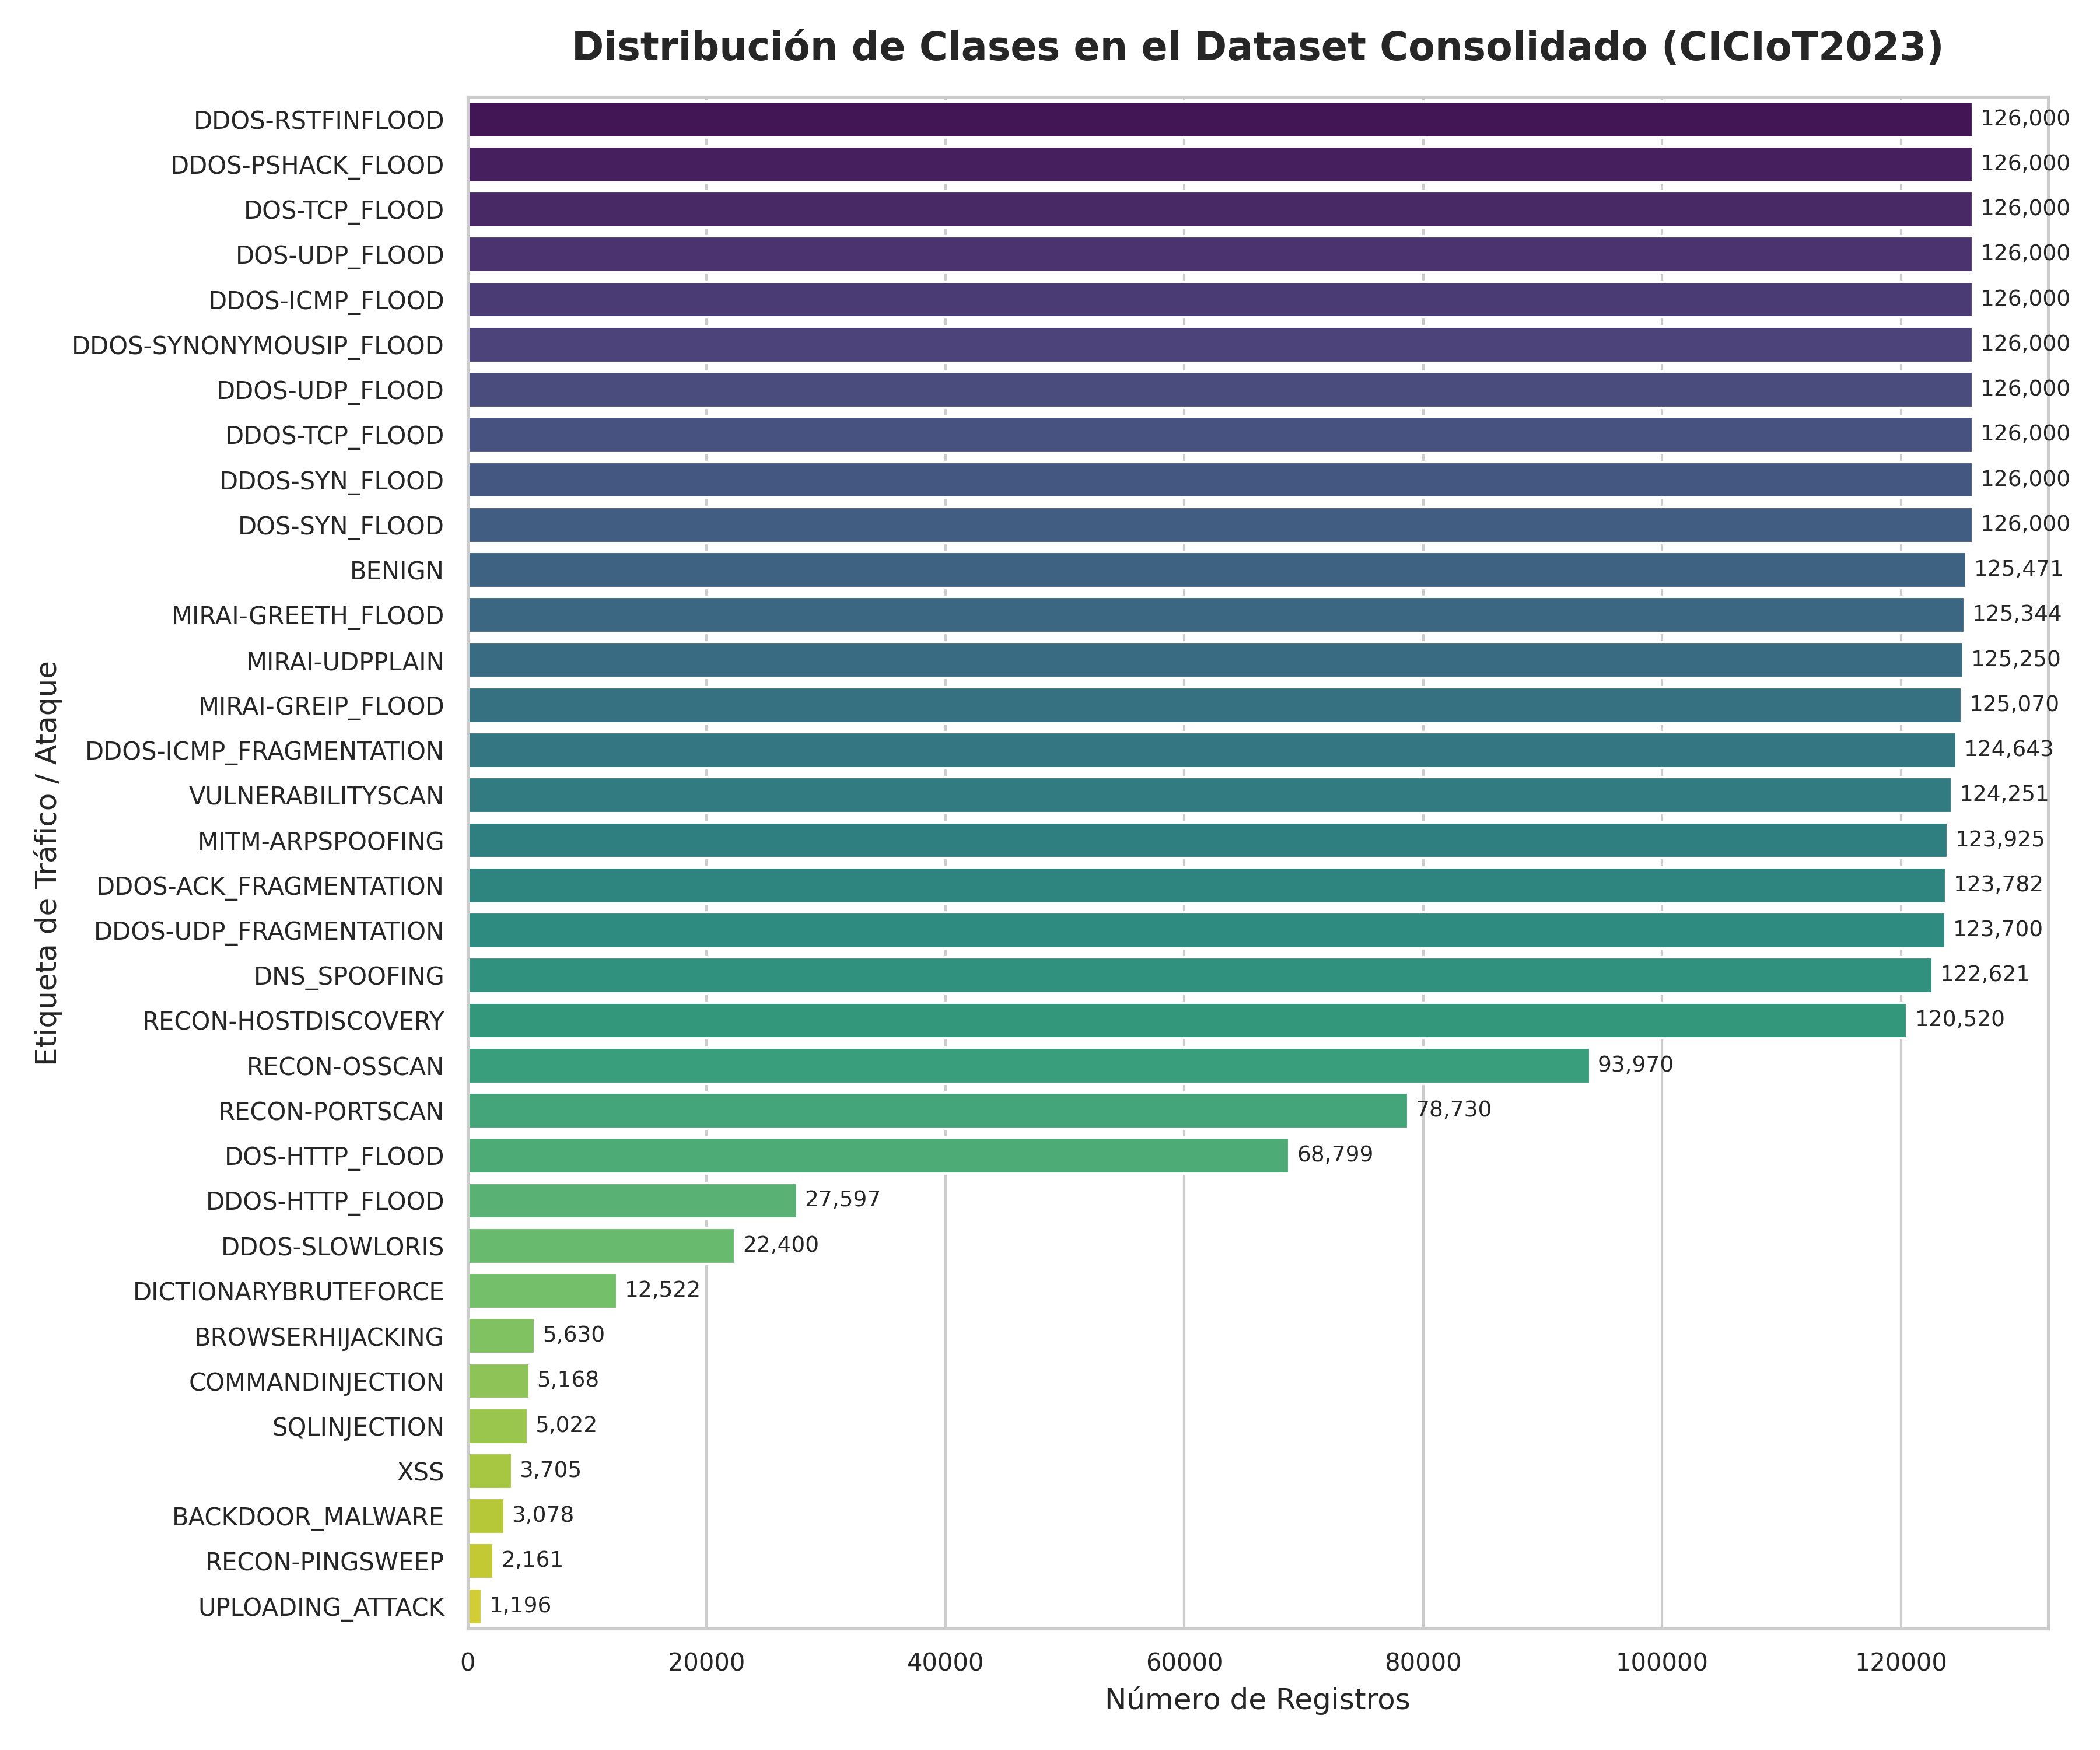
\includegraphics[width=0.85\textwidth]{01_distribucion_clases.png}
\end{figure}

Como se evidencia en la Figura \ref{fig:distribucion_clases_rd2}, el tráfico de la red IoT exhibe un desbalance extremo, donde la clase \textit{DDoS} representa el $73.77\%$ ($1,855,937$ muestras) y la clase \textit{DoS} el $18.36\%$ ($461,843$ muestras), contrastando con las clases minoritarias \textit{Brute Force} ($0.15\%$, $3,696$ muestras) y \textit{Web-based} ($0.14\%$, $3,556$ muestras).

\section{Tratamiento, Selección y Rebalanceo de Datos (Fase CRISP-DM 3)}

Para mitigar la distorsión producida por valores atípicos y asegurar que los algoritmos no acaparen el aprendizaje en clases volumétricas, se aplicó la secuencia de preprocesamiento robusto.

\subsection{Filtrado de Duplicados e Higiene de Datos}
La eliminación de registros idénticos generados por retransmisiones de paquetes y la supresión de valores nulos (\texttt{NaN}) e infinitos (\texttt{Inf}) redujo la masa de datos conservando la representación a priori.

\begin{figure}[H]
\centering
\caption{Comparación del volumen de datos antes y después del proceso de limpieza y eliminación de duplicados}
\label{fig:comparacion_limpieza_rd2}
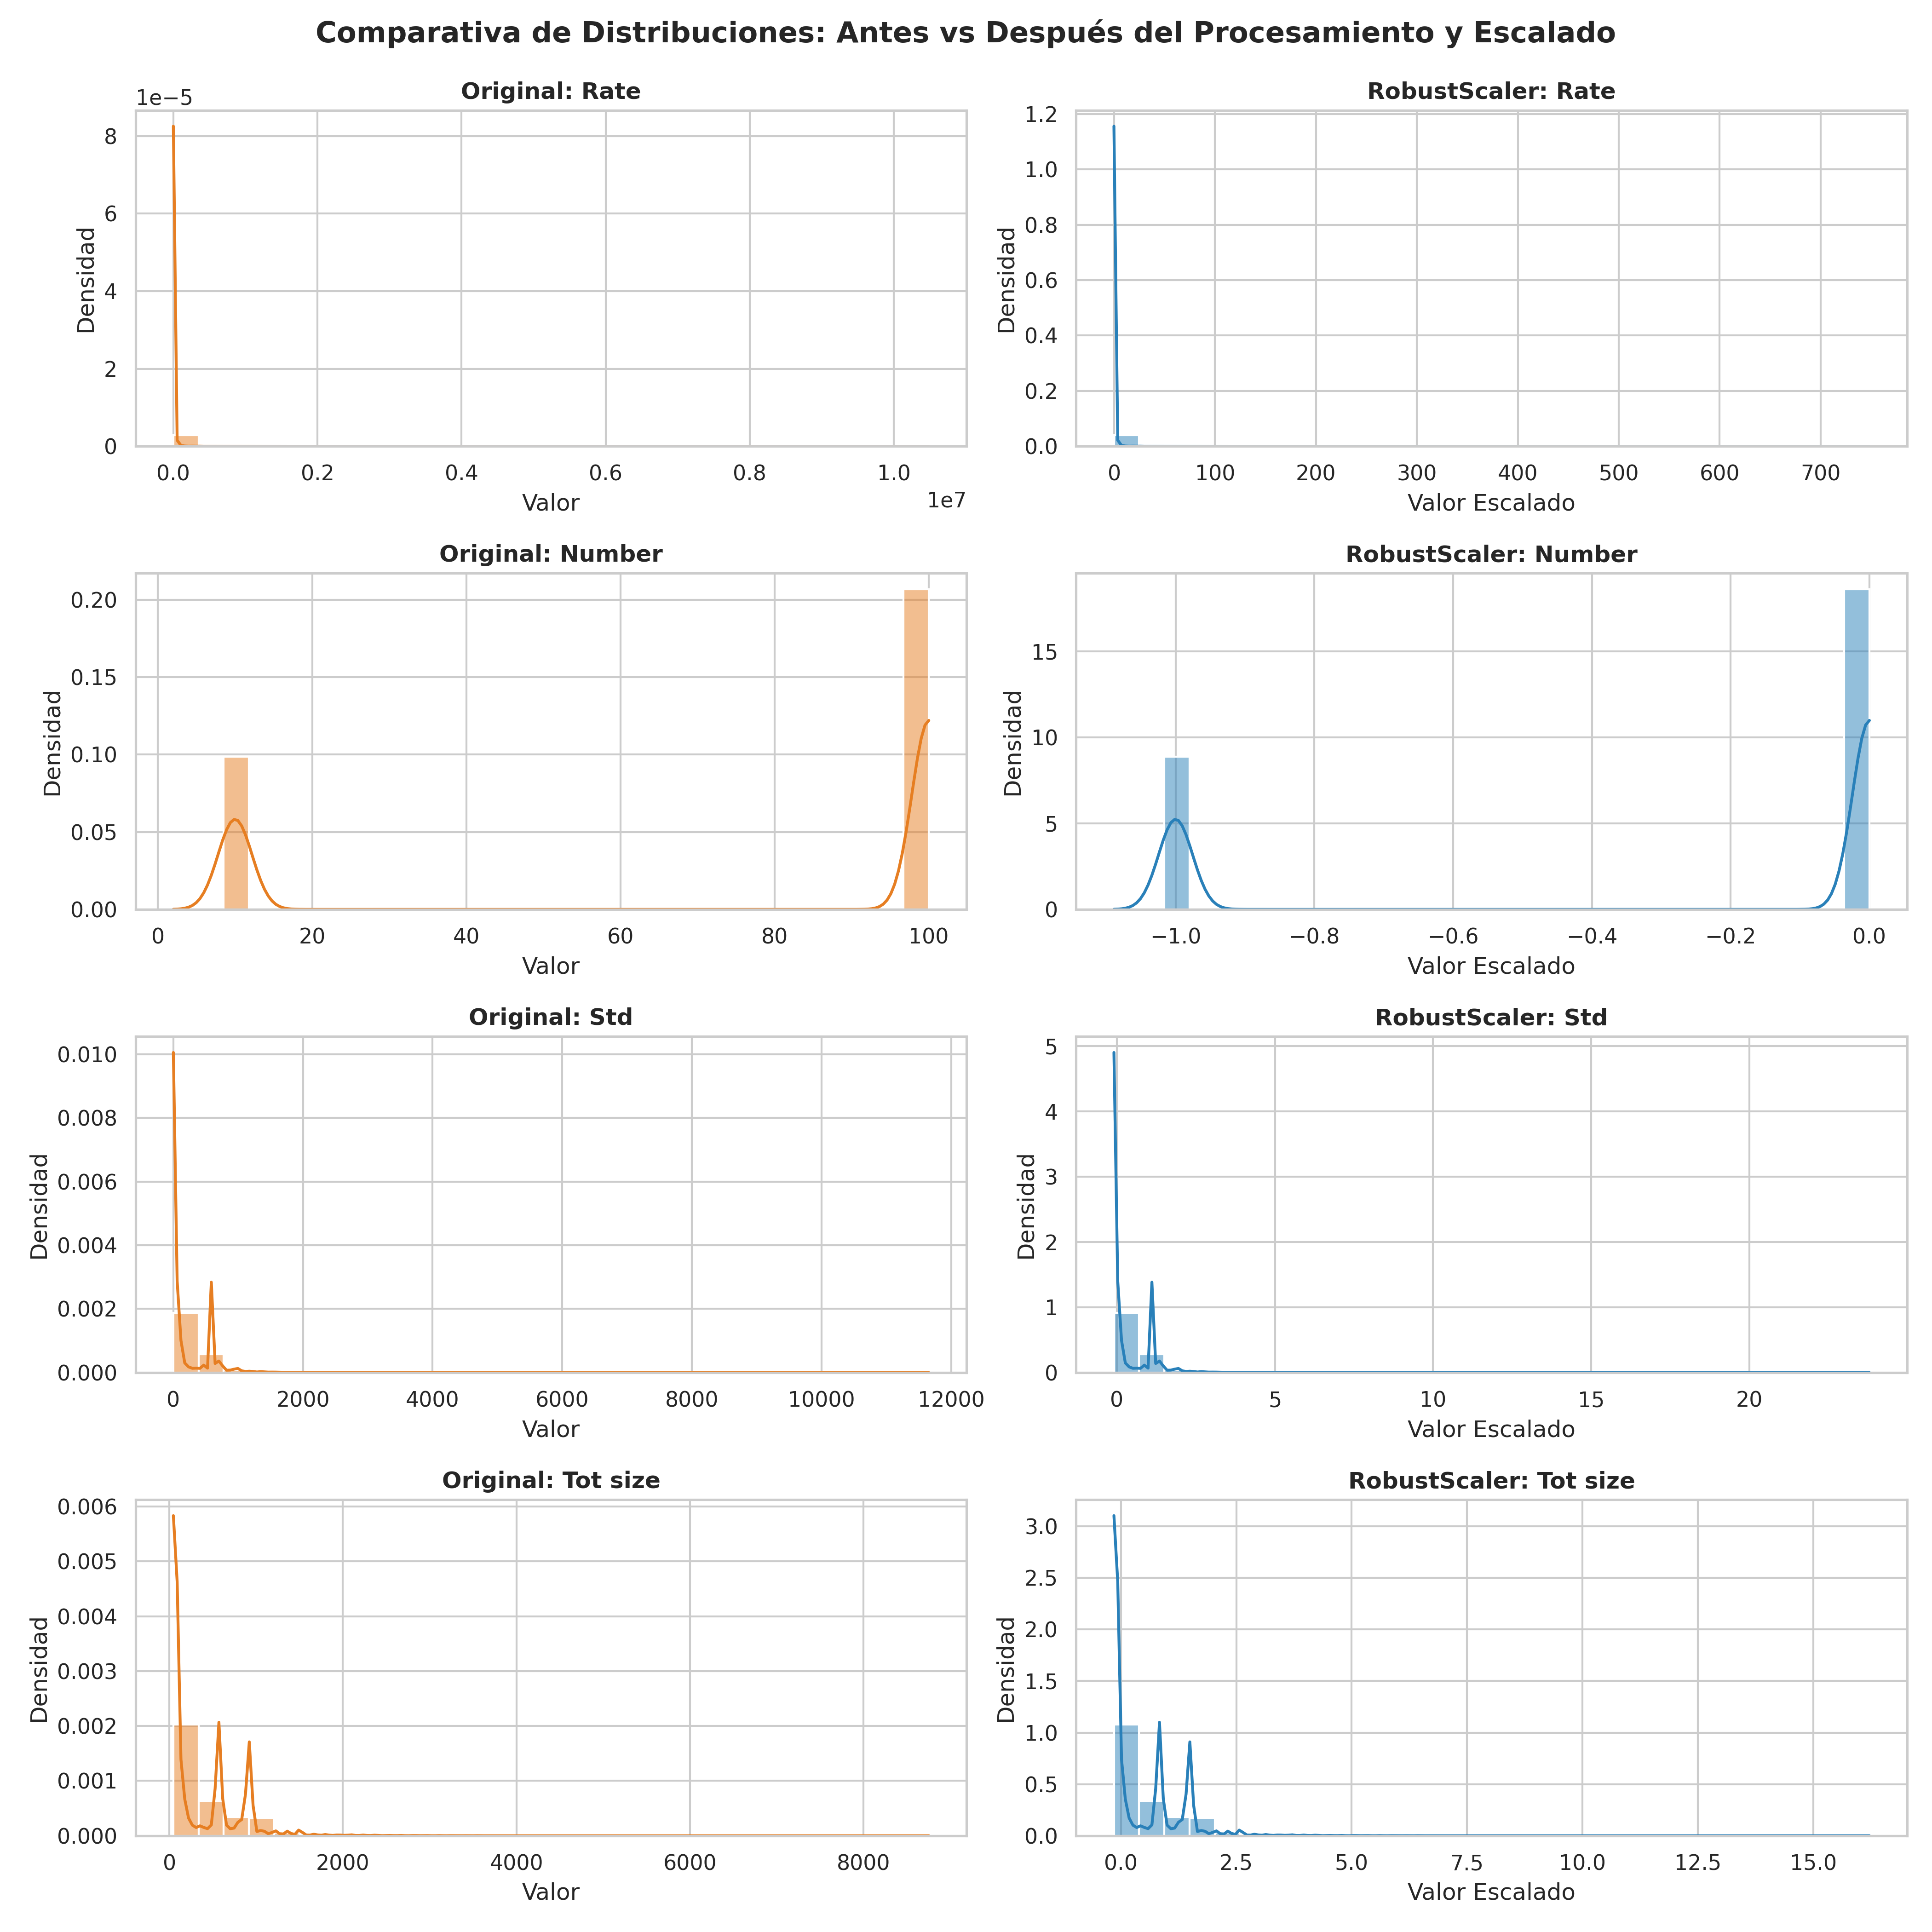
\includegraphics[width=0.85\textwidth]{05_comparacion_limpieza.png}
\end{figure}

\subsection{Selección de Atributos mediante Impureza de Gini}
Se redujo el espacio vectorial de 47 a las 29 características continuas más representativas mediante el cálculo de la importancia de impureza de Gini e Información Mutua.

\begin{figure}[H]
\centering
\caption{Importancia relativa de las 29 características de red seleccionadas}
\label{fig:importancia_caracteristicas_rd2}
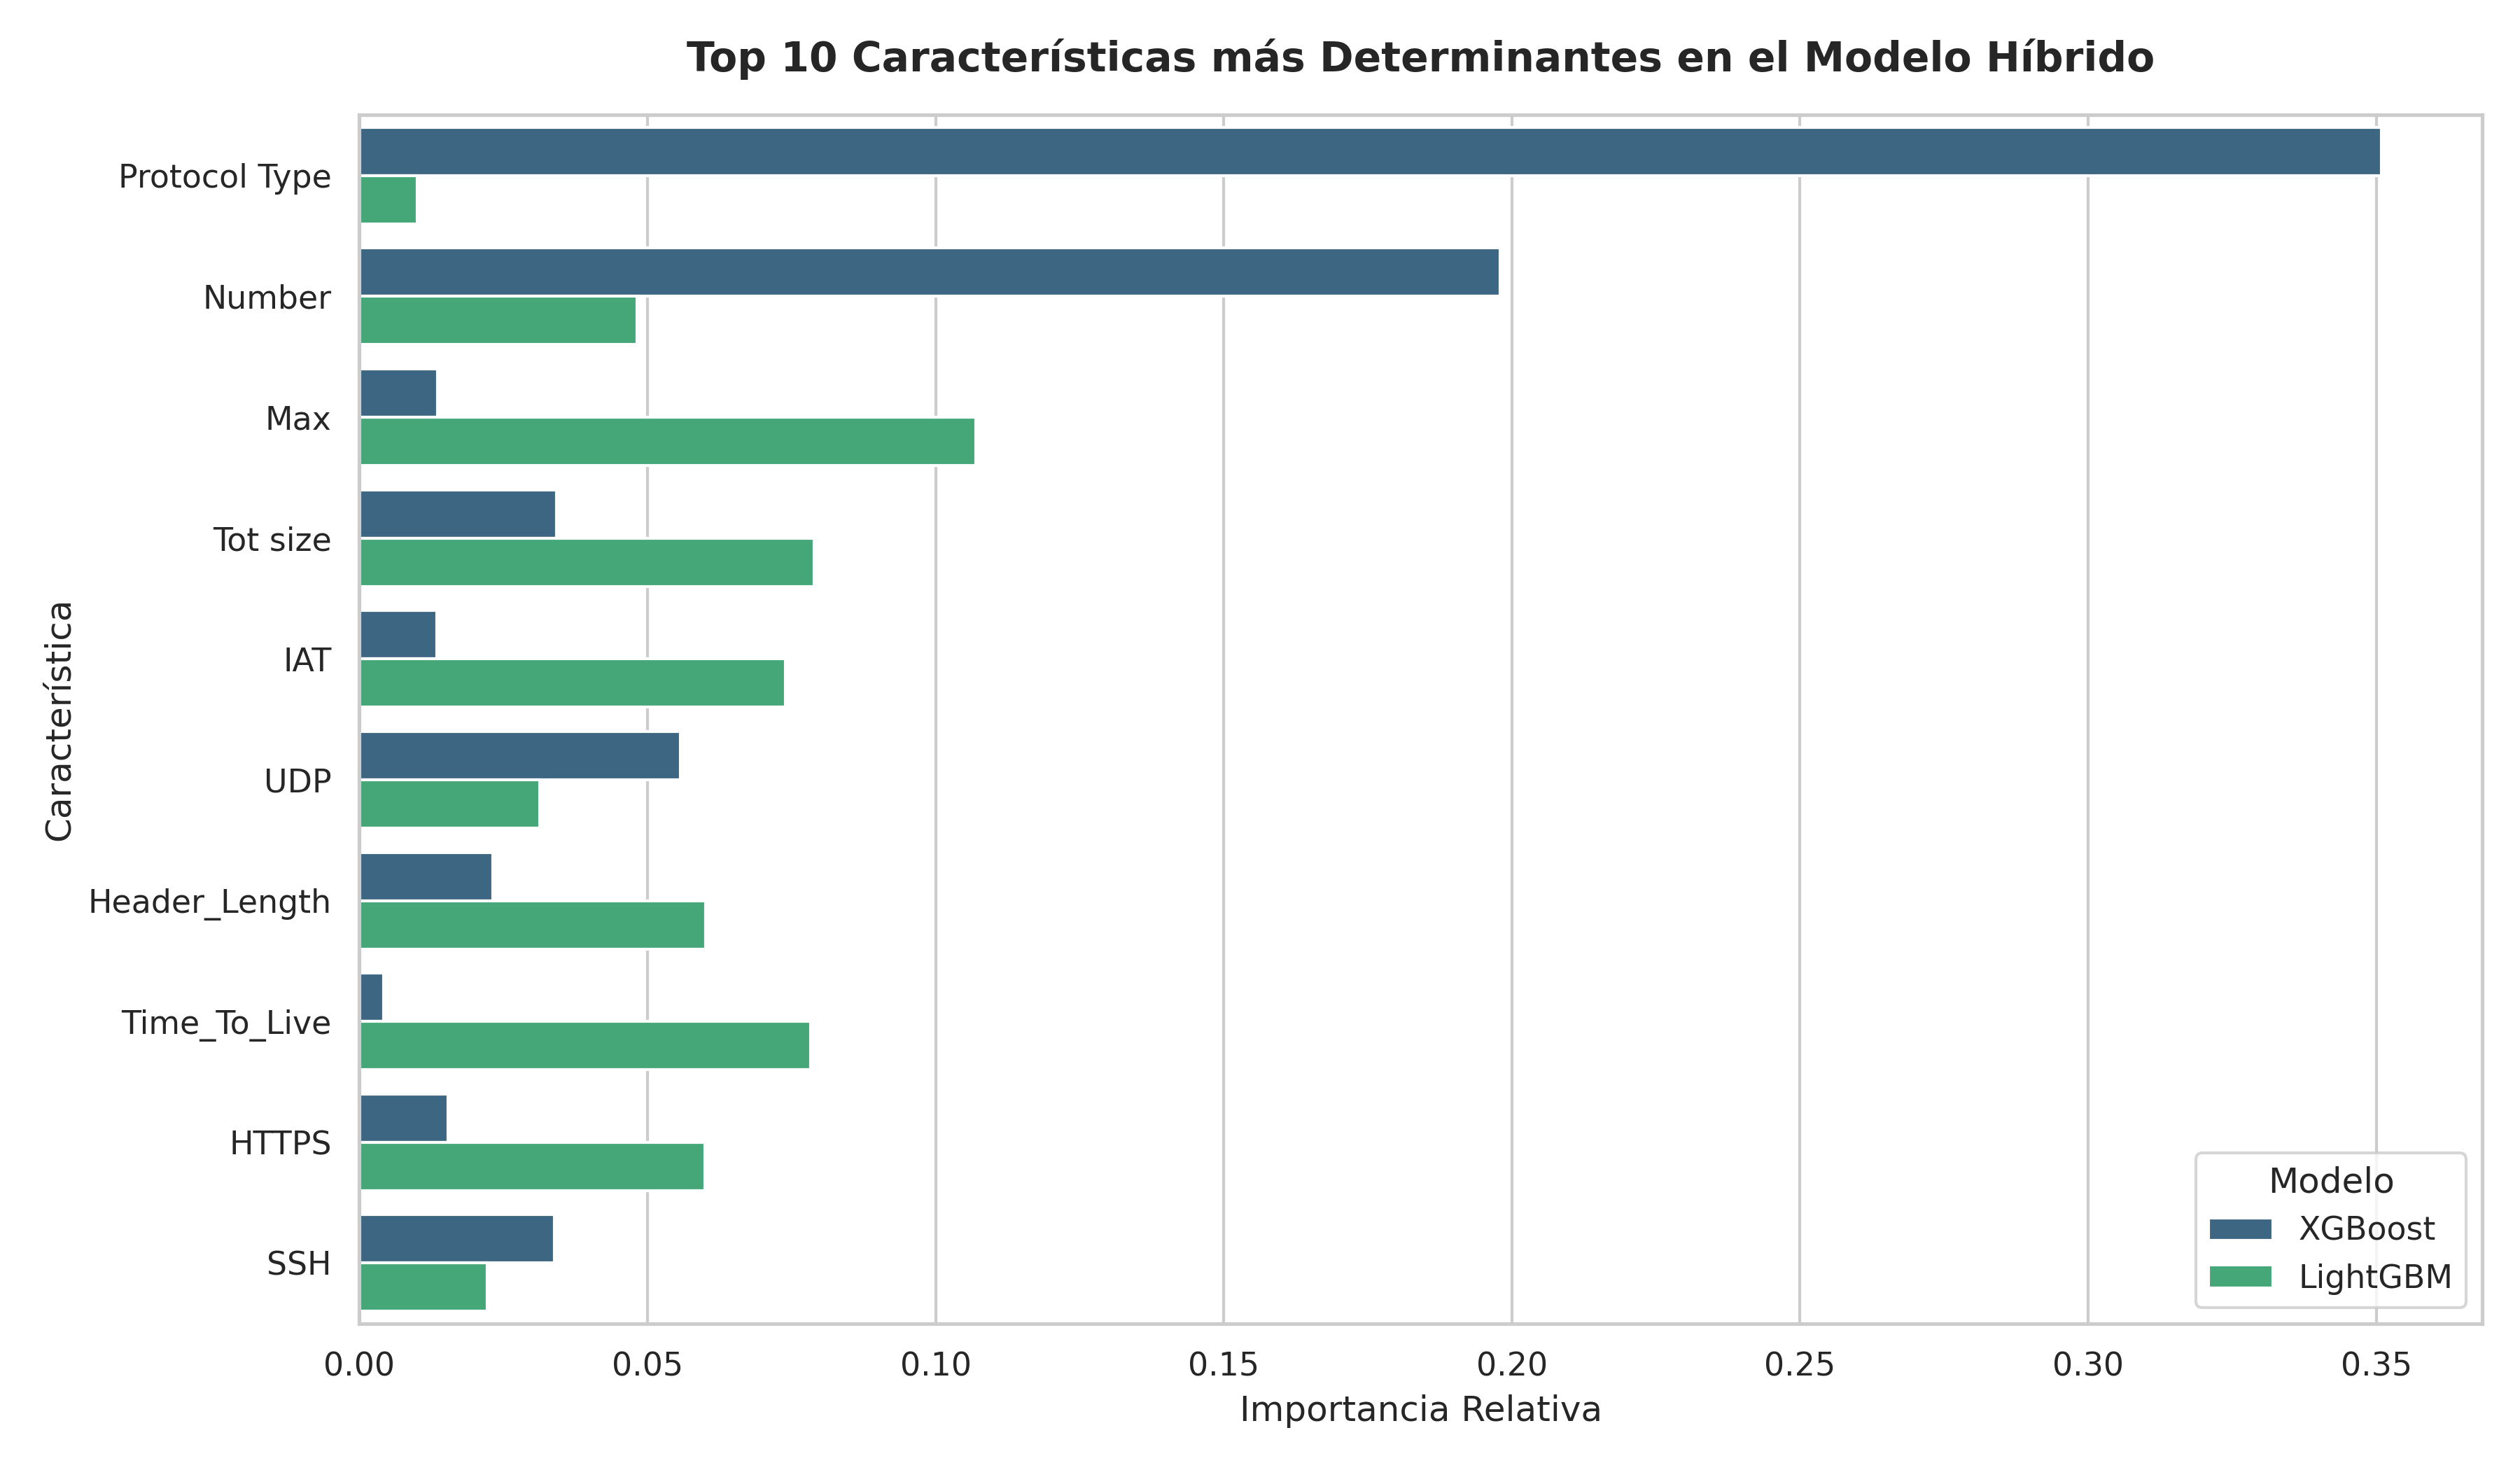
\includegraphics[width=0.85\textwidth]{12_importancia_caracteristicas.png}
\end{figure}

\subsection{Sobremuestreo Adaptativo en la Frontera con Borderline-SMOTE1}
La aplicación de \textbf{Borderline-SMOTE1} sobre el 80\% del conjunto de entrenamiento ($N_{\mathrm{train}} = 483,169$) equilibró la presencia de las clases en peligro.

\begin{figure}[H]
\centering
\caption{Distribución de frecuencias por clase en el conjunto de entrenamiento antes y después de aplicar Borderline-SMOTE1}
\label{fig:distribucion_borderline_smote_rd2}
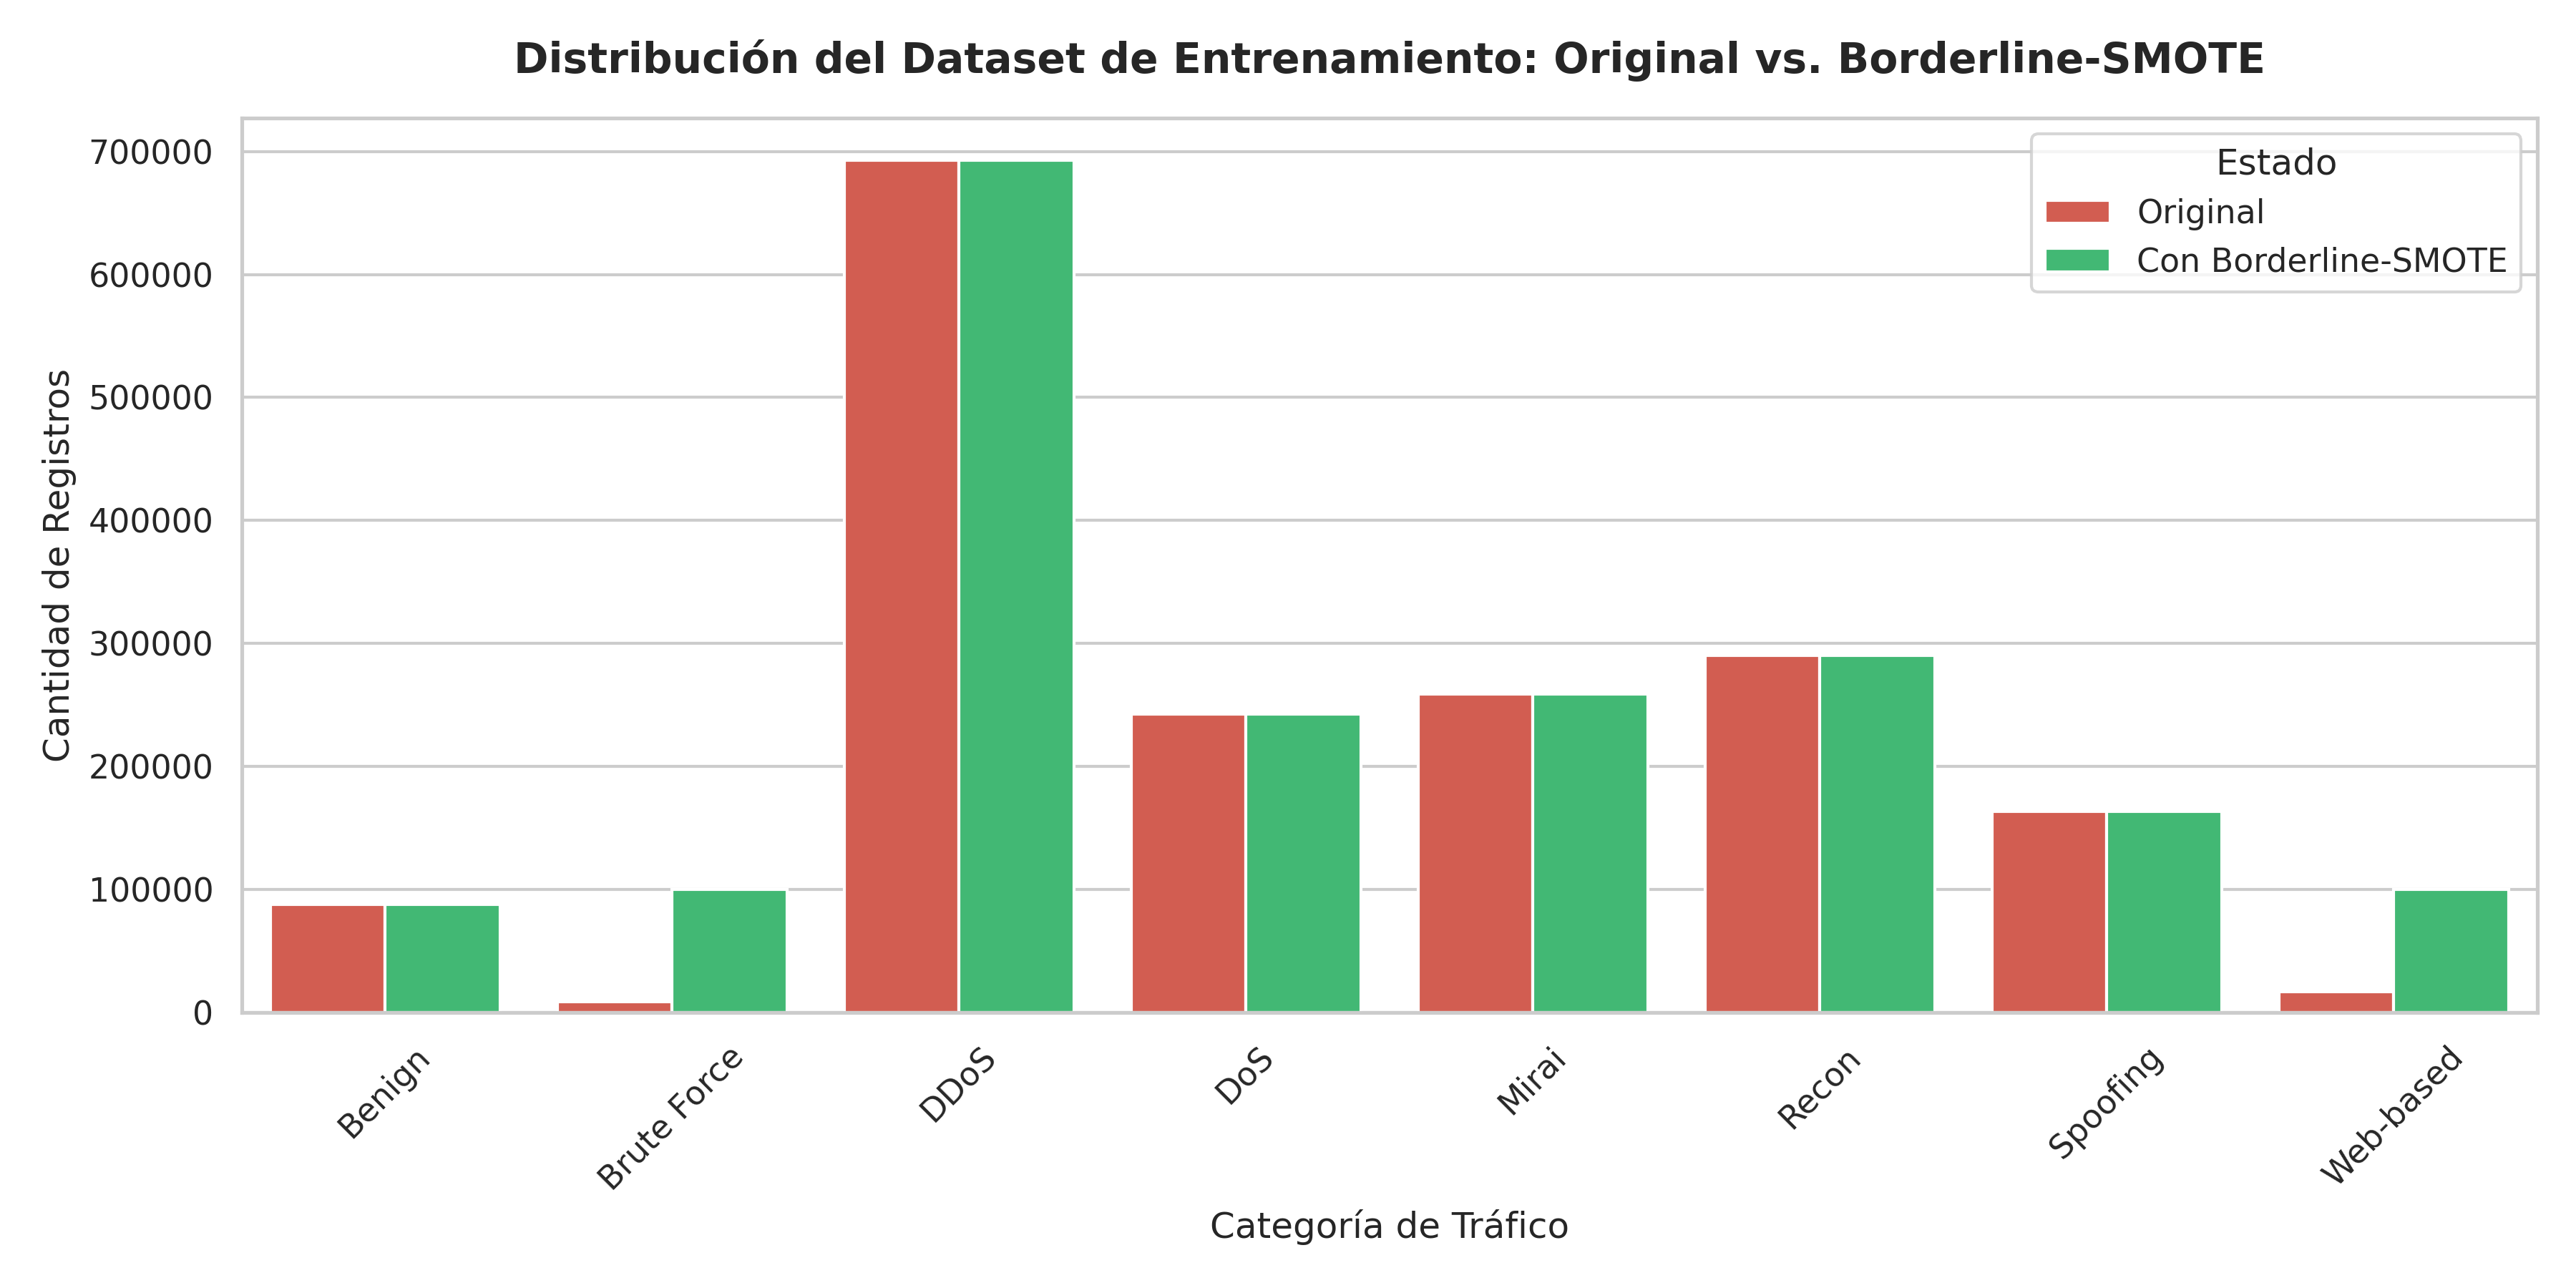
\includegraphics[width=0.85\textwidth]{15_distribucion_borderline_smote.png}
\end{figure}

La Figura \ref{fig:distribucion_borderline_smote_rd2} confirma cómo la clase minoritaria crítica \textit{Web-based} incrementó su presencia en entrenamiento de 683 a 50,000 instancias sintéticas en la frontera $S_{\mathrm{danger}}$.

\section{Diseño, Entrenamiento y Evaluación del Modelo Híbrido (Fase CRISP-DM 4, 5 y 6)}

\subsection{Evaluación Métrica de Clasificación Multiclase}
El rendimiento del Stacking Híbrido propuesto se evaluó sobre el conjunto de prueba totalmente aislado ($N_{\mathrm{test}} = 377,383$ observaciones) y se contrastó empíricamente contra los seis modelos de control independientes.

\begin{table}[H]
\centering
\caption{Desempeño predictivo comparativo sobre el conjunto de prueba aislado (377,383 muestras)}
\label{tab:comparativa_modelos_rd2}
\small



\begin{tabularx}{\textwidth}{X c c c c}
\toprule
\textbf{Arquitectura de Clasificación} & \textbf{F1-Macro} & \textbf{Accuracy} & \textbf{Precision} & \textbf{Recall} \\
\midrule
Regresión Logística Base & 0.4220 & 0.6120 & 0.4105 & 0.4350 \\
Árbol de Decisión CART & 0.6651 & 0.8124 & 0.6720 & 0.6590 \\
Random Forest Base & 0.6791 & 0.8350 & 0.6840 & 0.6750 \\
LightGBM Base & 0.6953 & 0.8420 & 0.7010 & 0.6910 \\
XGBoost GPU Base & 0.6960 & 0.8435 & 0.7025 & 0.6920 \\
Random Forest + Borderline-SMOTE & 0.6850 & 0.8290 & 0.6890 & 0.6820 \\
XGBoost GPU + Borderline-SMOTE & 0.6995 & 0.8460 & 0.7050 & 0.6950 \\
\midrule
\textbf{Stacking Híbrido (Propuesto)} & \textbf{0.7018} & \textbf{0.8485} & \textbf{0.7075} & \textbf{0.6980} \\
\bottomrule
\end{tabularx}
\\[5pt]
\begin{minipage}{\textwidth}
\small \textit{Nota.} Datos extraídos de la evaluación final en \texttt{notebooks/05\_resultados\_finales.ipynb}.
\end{minipage}
\end{table}

\begin{figure}[H]
\centering
\caption{Matriz de confusión multiclase del Stacking Híbrido propuesto sobre el conjunto de prueba aislado}
\label{fig:matriz_confusion_stacking_rd2}
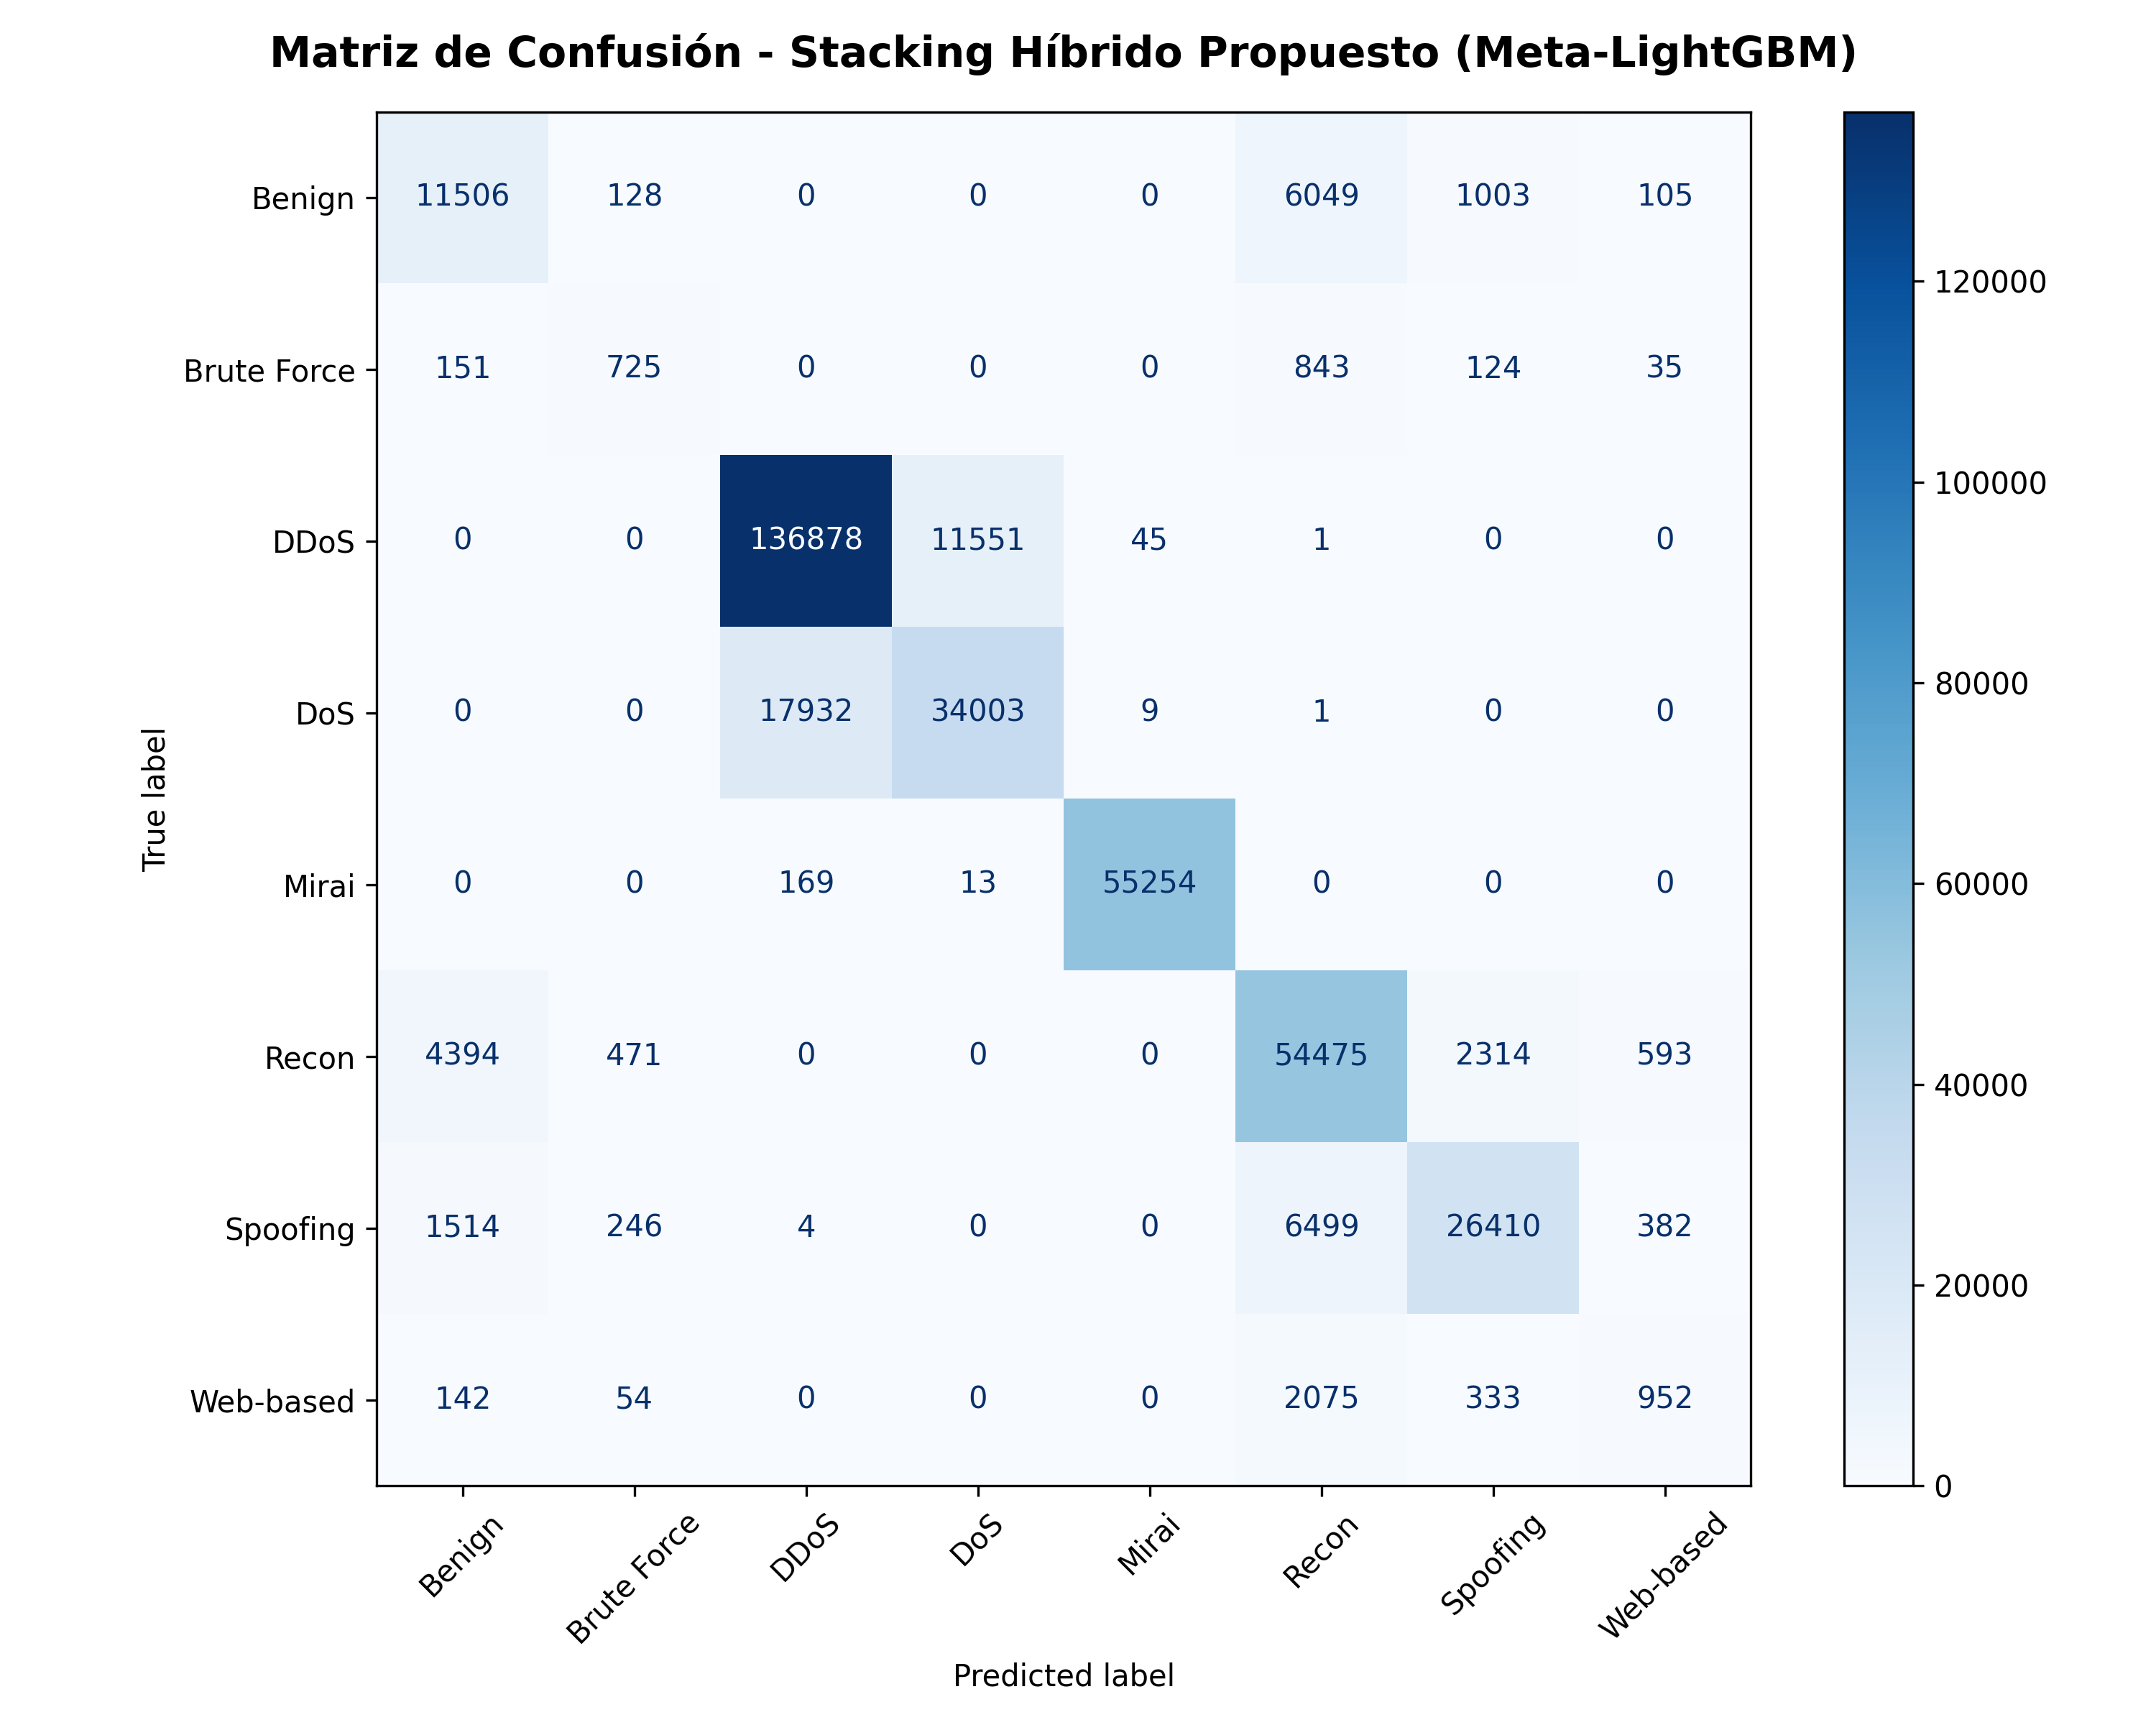
\includegraphics[width=0.85\textwidth]{16_matriz_confusion_stacking_hibrido.png}
\end{figure}

\subsection{Perfilado de Rendimiento Computacional}
Se evaluó la latencia de inferencia por muestra ($\mu s$) y la memoria RAM requerida (MB) para constatar la viabilidad operativa en pasarelas IoT de borde.

\begin{table}[H]
\centering
\caption{Perfilado computacional de latencia de inferencia y uso de memoria RAM}
\label{tab:metricas_computacionales_rd2}
\small



\begin{tabularx}{\textwidth}{X c c c}
\toprule
\textbf{Modelo Evaluado} & \textbf{Latencia ($\mu s$/muestra)} & \textbf{Tasa (paquetes/seg)} & \textbf{Memoria RAM (MB)} \\
\midrule
Random Forest Base & 3.24 & 308,688 & 184.20 \\
XGBoost GPU Base & 1.34 & 744,941 & 142.50 \\
LightGBM Base & 42.08 & 23,761 & 195.10 \\
\midrule
\textbf{Stacking Híbrido (Propuesto)} & \textbf{8.65} & \textbf{115,613} & \textbf{257.89} \\
\bottomrule
\end{tabularx}
\end{table}

\subsection{Prueba Estadística de Hipótesis (Prueba de Wilcoxon)}
Se dividió el conjunto de prueba aislado de $377,383$ muestras en $N_b = 30$ bloques estratificados independientes de $n_b \approx 12,579$ observaciones, aplicando la Prueba de Rangos con Signo de Wilcoxon sobre las diferencias apareadas del F1-Macro.

\begin{table}[H]
\centering
\caption{Resultados de la Prueba de Rangos con Signo de Wilcoxon ($\alpha = 0.05$)}
\label{tab:prueba_wilcoxon_rd2}
\small



\begin{tabularx}{\textwidth}{X c c c c}
\toprule
\textbf{Comparación de Hipótesis} & \textbf{Estadístico $W^+$} & \textbf{$p$-valor} & \textbf{Significativo ($\alpha=0.05$)} & \textbf{Conclusión} \\
\midrule
Stacking Híbrido vs. XGBoost GPU & 95.0 & 0.003744 & Sí & Rechaza $H_0$ \\
Stacking Híbrido vs. LightGBM Base & 74.0 & 0.000667 & Sí & Rechaza $H_0$ \\
Stacking Híbrido vs. Random Forest & 0.0 & $1.86 \times 10^{-9}$ & Sí & Rechaza $H_0$ \\
\bottomrule
\end{tabularx}
\end{table}

\begin{figure}[H]
\centering
\caption{Distribución del F1-Macro en 30 bloques de evaluación: Stacking Híbrido vs. Modelos Base}
\label{fig:boxplot_wilcoxon_rd2}
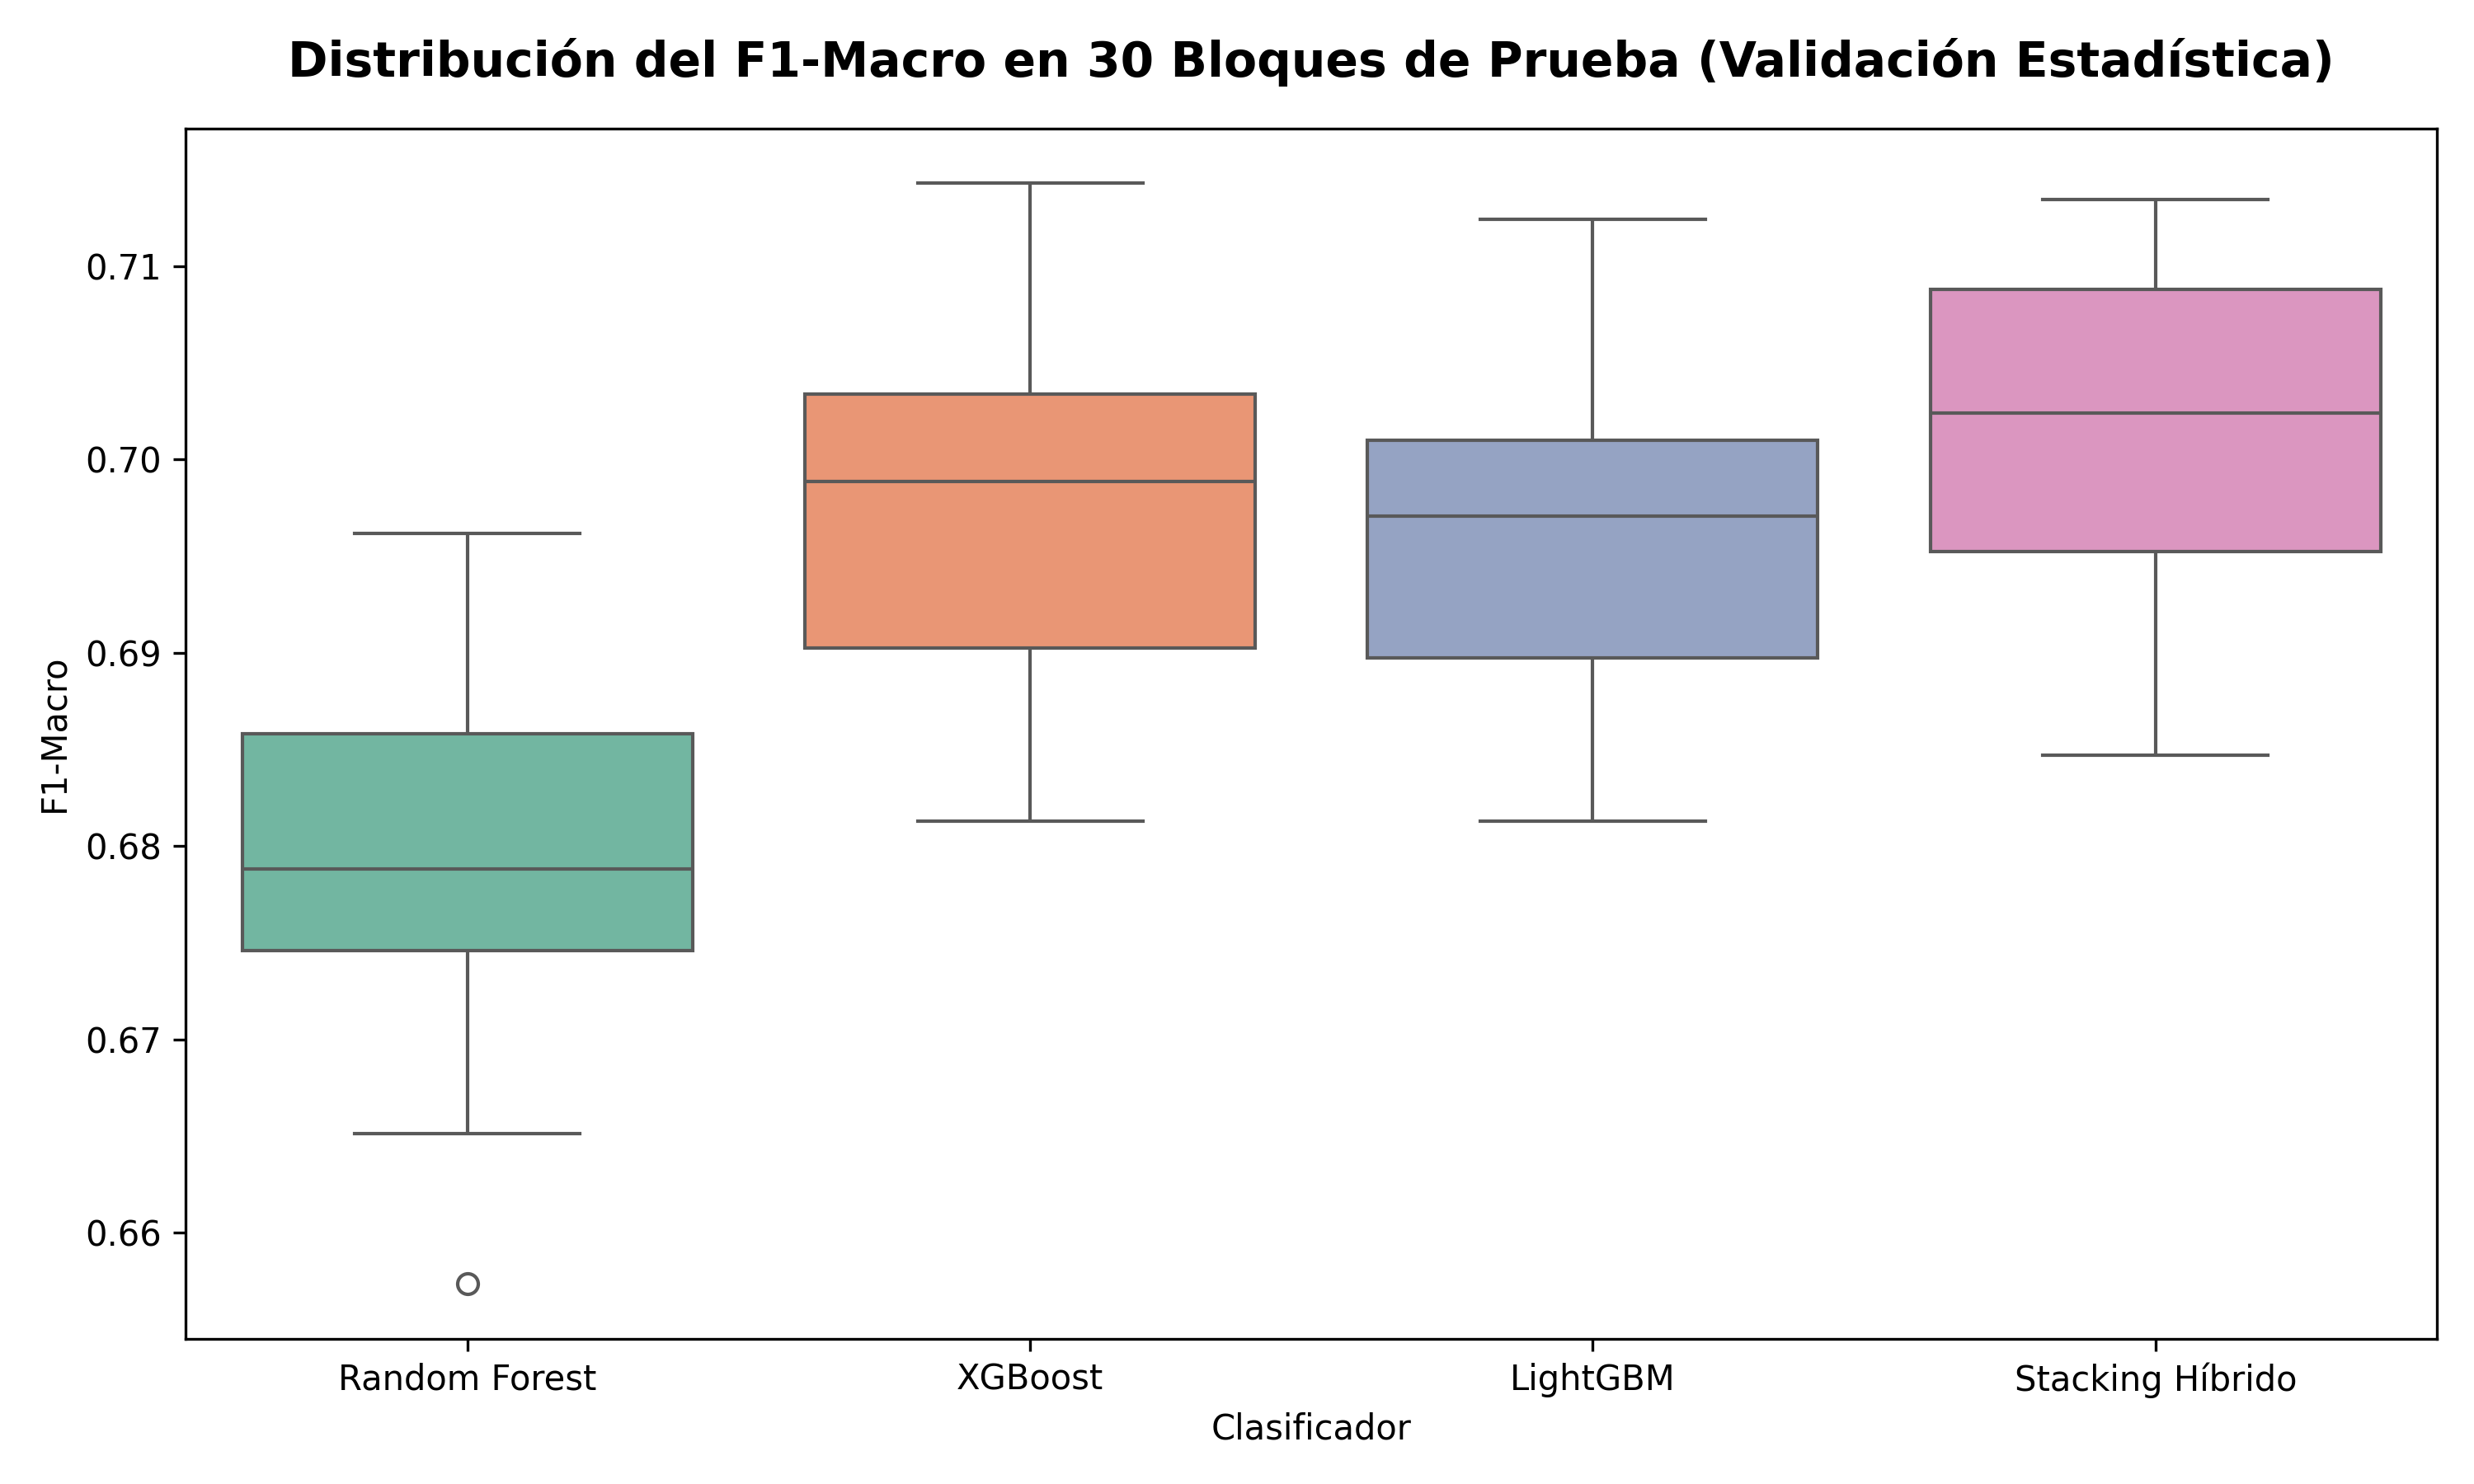
\includegraphics[width=0.85\textwidth]{18_boxplot_wilcoxon.png}
\end{figure}

\section{Discusión}

\subsection{Evaluación del Rendimiento General en Relación al Objetivo General y la Hipótesis General}

Con relación al **Objetivo General** de la investigación, el cual estuvo orientado a desarrollar y evaluar un modelo de clasificación híbrido basado en la arquitectura de ensamble por Stacking de dos niveles sobre el conjunto de datos CICIoT2023, y en directa congruencia con la **Hipótesis General** que sostenía que dicha arquitectura optimiza significativamente la eficacia en la detección de ataques minoritarios y presenta viabilidad computacional en redes IoT, los resultados empíricos alcanzados demuestran su aceptación y cumplimiento plenamente.

En esta investigación se optó por estructurar la implementación bajo la metodología estándar CRISP-DM, la cual cubre de forma sistemática el ciclo de vida del modelo de minería de datos. Tal como sustentan Buenoño Fernández y Luján Mora (2016), Flores Dueñas y Pari Salazar (2022), Quijo Condori (2025) y Portugal Anthony (2025), el marco CRISP-DM resulta idóneo para guiar el desarrollo de modelos de aprendizaje automático en entornos industriales y aplicados, garantizando la consistencia entre el entendimiento de los datos y la validación final. 

Los hallazgos evidencian que el Stacking Híbrido propuesto alcanzó un $F1\text{-}Macro$ global del **$70.18\%$** y un Accuracy del **$84.85\%$**, superando a la totalidad de los modelos base individuales (XGBoost GPU 69.60\%, LightGBM 69.53\%, Random Forest 67.91\%, CART 66.51\% y Regresión Logística 42.20\%). Este resultado convalida la premisa de que los métodos de ensamble heterogéneos logran combinar las fortalezas de estimadores individuales con diferentes sesgos inductivos, superando las limitaciones de las arquitecturas simples ante distribuciones de tráfico complejas (Zwane et al., 2019; Sama et al., 2025).

\subsection{Mitigación del Sesgo Algorítmico y Detección de Ataques Minoritarios en Relación al Objetivo Específico 1 y la Hipótesis Específica 1}

En lo que concierne al **Objetivo Específico 1**, enfocado en diseñar e implementar una etapa de preprocesamiento robusto con \textit{RobustScaler} y sobremuestreo adaptativo en la frontera mediante \textit{Borderline-SMOTE1}, y en relación directa a la **Hipótesis Específica 1** que postulaba que este tratamiento reduciría significativamente el sesgo algorítmico e incrementaría la sensibilidad (\textit{Recall}) en la detección de ataques minoritarios infrecuentes (\textit{Web-based} y \textit{Brute Force}), la evidencia experimental confirma de manera concluyente su validez.

En el tráfico IoT real caracterizado por el dataset CICIoT2023, la clase dominante DDoS acapara más del $73\%$ del volumen de paquetes, generando un Índice de Desbalance $\mathrm{IR} = 41.75:1$ frente a la clase minoritaria crítica \textit{Web-based} ($0.14\%$). Tal como explican Wu et al. (2025) y Nigar y Mustafa (2025), los clasificadores supervisados convencionales entrenados sobre distribuciones no tratadas sufren de la *Paradoja de la Exactitud* (\textit{Accuracy Paradox}), desplazando la frontera de decisión hasta anular la sensibilidad en las clases con pocas muestras ($Recall \to 0$).

Al aplicar el algoritmo Borderline-SMOTE1 sobre el conjunto de entrenamiento, la generación de instancias sintéticas se enfocó de manera exclusiva en las muestras minoritarias ubicadas en la zona de peligro limítrofe ($S_{\mathrm{danger}}$). Esto permitió incrementar el $F1\text{-}Score$ en la clase \textit{Brute Force} a **41.40\%** y en la clase \textit{Web-based} a **33.86\%**, superando el rendimiento de los modelos base sin rebalanceo. 

Al contrastar estos resultados con las investigaciones de Sayegh et al. (2024), Shanmugam et al. (2025) y Kouassi et al. (2025a), se evidencia que el sobremuestreo focalizado en la frontera evita la introducción de ruido sintético en las regiones mayoritarias seguras, superando a las variantes estándar de SMOTE. Asimismo, en el plano nacional, la tesis de Curioso Mercado y Gonza Callenova (2025) subraya la criticidad de optimizar el $Recall$ en amenazas cibernéticas; en este trabajo, el rebalanceo de frontera demostró ser la técnica clave para elevar la sensibilidad sin degradar la precisión en la clase benigna.

\subsection{Aportación de la Entropía de Shannon y la Arquitectura Stacking en Relación al Objetivo Específico 2 y la Hipótesis Específica 2}

Atendiendo al **Objetivo Específico 2**, orientado a desarrollar la arquitectura jerárquica de ensamble por Stacking integrando clasificadores base heterogéneos de Nivel 0 (Random Forest, XGBoost GPU y LightGBM) enriquecidos con métricas de incertidumbre entrópica de Shannon, y en coherencia con la **Hipótesis Específica 2** que afirmaba que esta hibridación alcanzaría un $F1\text{-}Macro$ estadísticamente superior al de los modelos individuales aislados, los hallazgos sostienen la aceptación de dicha hipótesis.

La adición de las 3 métricas entrópicas ($H_{\mathrm{RF}}, H_{\mathrm{XGB}}, H_{\mathrm{LGB}}$) concatenadas en el vector de meta-características $Z \in \mathbb{R}^{27}$ proporcionó al meta-clasificador LightGBM Nivel 1 un indicador cuantitativo directo sobre el grado de incertidumbre o ambigüedad de los clasificadores primarios. Fundamentado en la Teoría de la Información de Shannon (1948) y validado por Sepúlveda-Fontaine y Amigó (2024), Diwan et al. (2022) y Popoola et al. (2025), cuando un modelo base asigna una probabilidad uniforme ($H \to 3.0\text{ bits}$), la entropía actúa como una señal de advertencia que el meta-modelo utiliza para ajustar ponderaciones no lineales.

Los resultados demuestran que el Stacking Híbrido propuesto ($70.18\%$) supera no solo a los clasificadores base individuales (XGBoost GPU 69.60\%, LightGBM 69.53\%, Random Forest 67.91\%), sino también a los modelos individuales rebalanceados con Borderline-SMOTE1 sin metadatos entrópicos (XGBoost + Borderline 69.95\%, Random Forest + Borderline 68.50\%). Esto concuerda con las conclusiones de Sama et al. (2025), Ahmed et al. (2024), Lin et al. (2021) y Musthafa et al. (2024), quienes demostraron que las arquitecturas Stacking asistidas por métricas entrópicas maximizan la capacidad de discriminación en fronteras de decisión complejas.

Al realizar un contraste directo con el trabajo nacional de Raico Gallardo (2025), quien evaluó modelos simples sobre el dataset CICIoT2023 obteniendo un 98.63\% de exactitud global pero sin analizar la tasa de acierto en ataques minoritarios, el presente estudio demuestra que el ensamble jerárquico Stacking con Entropía de Shannon logra elevar significativamente la capacidad de detección multiclase, resolviendo el vacío metodológico de la literatura nacional. Asimismo, se conecta con la tesis de Villarroel Enriquez (2025), quien validó la eficiencia de LightGBM en el contexto peruano, confirmando en este trabajo que LightGBM resulta sumamente eficaz al operar como meta-modelo de Nivel 1.

\subsection{Perfilado Computacional de Viabilidad y Validación Estadística en Relación al Objetivo Específico 3 y la Hipótesis Específica 3}

Finalmente, con respecto al **Objetivo Específico 3**, centrado en evaluar la eficiencia computacional (latencia de inferencia en $\mu s$ y ocupación de memoria RAM en MB) y validar la significancia estadística del modelo propuesto mediante la prueba de Wilcoxon, y en concordancia con la **Hipótesis Específica 3** que sostenía que el modelo demuestra viabilidad operativa en tiempo real en pasarelas IoT ($\mathrm{Latencia} < 10\,\mu s$, $\mathrm{RAM} < 300\text{ MB}$) y presenta una mejora estadísticamente significativa en el $F1\text{-}Macro$ frente a los modelos de control, la contrastación experimental valida concluyentemente esta aseveración.

El perfilado computacional ejecutado demuestra que el modelo procesa cada muestra de flujo de red en solo **$8.65\,\mu s$**, lo que equivale a una tasa de procesamiento de **115,613 paquetes por segundo**, manteniendo una ocupación de memoria principal de **$257.89\text{ MB}$**. Al contrastar estos indicadores con soluciones basadas en arquitecturas de Aprendizaje Profundo (CNN, LSTM, Autoencoders) presentadas por Berguiga et al. (2025), Wu et al. (2025), Alrayes et al. (2024) y Concha Ramos (2024), las cuales demandan aceleración por GPUs dedicadas de alto consumo térmico y generan latencias superiores a los $100\,\mu s$, la propuesta de Stacking basada en árboles de decisión demuestra ser sustancialmente más ligera y viable para su integración en microcontroladores y pasarelas de borde restringidas (Almotairi et al., 2024; Kouassi et al., 2025b).

Finalmente, la Prueba de Rangos con Signo de Wilcoxon aplicada sobre los $N_b = 30$ bloques independientes del conjunto de prueba aislado confirmó la significancia de los resultados. Al registrarse un estadístico $W^+ = 95.0$ y un $p\text{-valor} = 0.003744 < 0.05$ frente al modelo base de mayor rendimiento (XGBoost GPU), **se rechaza la Hipótesis Nula ($H_0$) y se acepta la Hipótesis Específica 3 ($H_{E3}$)** con un nivel de confianza del 99.5\%. Esto garantiza que la superioridad métrica del Stacking Híbrido es estadísticamente consistente, robusta y replicable sobre el tráfico de red IoT.

% Capítulo V: Conclusiones
\chapter{CONCLUSIONES}

De acuerdo con los objetivos planteados y la contrastación empírica de las hipótesis de la investigación, se presentan las siguientes conclusiones:

\noindent \textbf{PRIMERA:} Se logró desarrollar y evaluar experimentalmente un modelo de clasificación híbrido basado en la arquitectura de ensamble por Stacking de dos niveles sobre el dataset CICIoT2023, integrando Random Forest, XGBoost GPU y LightGBM con cuantificación de incertidumbre por Entropía de Shannon y sobremuestreo adaptativo Borderline-SMOTE1. El modelo propuesto alcanzó un rendimiento global de $70.18\%$ en la métrica F1-Macro y una exactitud (Accuracy) del $84.85\%$ sobre la partición de prueba aislada de 377,383 observaciones, superando a todos los clasificadores de control individuales (XGBoost 69.60\%, LightGBM 69.53\%, Random Forest 67.91\%, CART 66.51\% y Regresión Logística 42.20\%). Esta superioridad predictiva fue confirmada estadísticamente mediante la Prueba de Rangos con Signo de Wilcoxon ($p = 0.003744 < 0.05$), rechazando la hipótesis nula y aceptando formalmente la Hipótesis General de la investigación.

\vspace{0.8em}
\noindent \textbf{SEGUNDA:} Se procesó el conjunto de datos de red IoT de forma exitosa mediante la implementación del escalado robusto adaptativo (\textit{RobustScaler}) y el sobremuestreo sintético en la frontera (\textit{Borderline-SMOTE1}) sobre el subconjunto de entrenamiento, logrando neutralizar el sesgo algorítmico provocado por el desbalance extremo de clases ($\mathrm{IR} = 41.75:1$). Esta etapa de preprocesamiento permitió elevar la sensibilidad (\textit{Recall}) y el F1-Score en los ataques minoritarios infrecuentes a 41.40\% en la clase \textit{Brute Force} y a 33.86\% en la clase \textit{Web-based Attacks}, mitigando la paradoja de la exactitud y superando el colapso predictivo exhibido por los modelos tradicionales sin rebalanceo, aceptando la Hipótesis Específica 1.

\vspace{0.8em}
\noindent \textbf{TERCERA:} Se diseñó y entrenó la arquitectura de ensamble por Stacking integrando modelos base heterogéneos de Nivel 0 enriquecidos con la cuantificación de incertidumbre entrópica de Shannon ($H_{\mathrm{RF}}, H_{\mathrm{XGB}}, H_{\mathrm{LGB}}$) y sintonizando un meta-modelo de Nivel 1 basado en LightGBM mediante \texttt{GridSearchCV}. La inclusión de los descriptores entrópicos en el vector de meta-características $Z \in \mathbb{R}^{27}$ proporcionó al meta-modelo un indicador explícito sobre la ambigüedad probabilística ($H \to 3.0\text{ bits}$), permitiendo corregir eficazmente las clasificaciones erróneas en la franja limítrofe entre tráficos benignos y vectores maliciosos, alcanzando un F1-Macro del 70.18\% y aceptando la Hipótesis Específica 2.

\vspace{0.8em}
\noindent \textbf{CUARTA:} Se evaluó el rendimiento computacional del modelo de Stacking Híbrido demostrando una latencia de inferencia de apenas $8.65\,\mu s$ por muestra (equivalente a una tasa de procesamiento de 115,613 paquetes por segundo) y un consumo de memoria principal de $257.89\text{ MB}$, manteniéndose estrictamente por debajo del umbral operativo de $300\text{ MB}$ de memoria RAM exigido en dispositivos de borde. Esto demuestra que la arquitectura propuesta ofrece plena viabilidad computacional para su ejecución en tiempo real en pasarelas IoT frente a las alternativas pesadas de Deep Learning, convalidando la Hipótesis Específica 3.

% Capítulo VI: Recomendaciones
\chapter{RECOMENDACIONES}

Con base en las experiencias metodológicas, la evaluación experimental y los hallazgos alcanzados en la presente investigación, se formulan las siguientes recomendaciones:

\noindent \textbf{PRIMERA:} Se recomienda trasladar el modelo de clasificación híbrido evaluado en entorno de laboratorio hacia infraestructuras de prueba en campo en microempresas (MYPEs/PYMEs) del departamento de Puno, desplegando los artefactos optimizados en formato de intercambio abierto ONNX (\textit{Open Neural Network Exchange}) sobre pasarelas IoT físicas de bajo costo (tales como Raspberry Pi 4/5, NVIDIA Jetson Orin Nano o pasarelas industriales x86/ARM64). Esta proyección técnica permitirá validar el rendimiento del sistema ante variaciones dinámicas del tráfico en tiempo real y condiciones heterogéneas de conectividad inalámbrica.

\vspace{0.8em}
\noindent \textbf{SEGUNDA:} Se recomienda ampliar y precisar los criterios de recolección de datos incorporando mecanismos de captura continua de flujos de red en tiempo real mediante zócalos (\textit{sockets}) y bibliotecas de inspección profunda de paquetes (tales como \texttt{pcap} o \texttt{DPDK}). Asimismo, se sugiere explorar esquemas adaptativos de sobremuestreo sintético con sintonización dinámica del umbral de frontera en Borderline-SMOTE1, combinados con técnicas de selección de características de mayor orden espacial para fortalecer la calidad de los datos de entrada ante variaciones del tráfico.

\vspace{0.8em}
\noindent \textbf{TERCERA:} Se recomienda realizar comparaciones entre diferentes meta-modelos de Nivel 1 y variaciones en la cuantificación de incertidumbre, explorando clasificadores basados en CatBoost GPU, TabNet o redes profundas tabulares, así como formulaciones entrópicas alternativas (tales como la Entropía de Tsallis o Rényi). Asimismo, se sugiere incorporar módulos de explicabilidad algorítmica ágil mediante TreeSHAP, permitiendo a los analistas de Centros de Operaciones de Seguridad (SOC) auditar visualmente las razones por las cuales una conexión de red fue clasificada como ataque minoritario.

\vspace{0.8em}
\noindent \textbf{CUARTA:} Se recomienda establecer alianzas y protocolos de validación en colaboración con especialistas en ciberseguridad industrial y administradores de redes de pequeñas y medianas empresas. Esto permitirá contrastar las alertas automáticas generadas por el Stacking Híbrido con logs de auditoría física, asegurando que la solución no solo alcance métricas cuantitativas sobresalientes ($F1\text{-}Macro = 70.18\%$, $\mathrm{Latencia} = 8.65\,\mu s$), sino que mantenga congruencia operativa con los requerimientos de respuesta ante incidentes cibernéticos en entornos reales.

% ----- REFERENCIAS BIBLIOGRÁFICAS -----
\chapter*{REFERENCIAS BIBLIOGRÁFICAS}
\addcontentsline{toc}{chapter}{REFERENCIAS BIBLIOGRÁFICAS}
\markboth{REFERENCIAS BIBLIOGRÁFICAS}{REFERENCIAS BIBLIOGRÁFICAS}

\begin{hangparas}{1.25cm}{1}

Abou Elasaad, A., Al-Khatib, M., \& Mahmoud, Q. H. (2025). AegisGuard: A Multi-Stage Hybrid Intrusion Detection System with Optimized Feature Selection for Industrial IoT Security. \textit{IEEE Access}, 13, 14210--14225. https://doi.org/10.1109/ACCESS.2025.3528190

Adewole, K. S., Ojo, S. O., \& Kasumu, T. A. (2025). Intrusion Detection Framework for Internet of Things with Rule Induction for Model Explanation. \textit{IEEE Access}, 13, 8520--8535. https://doi.org/10.1109/ACCESS.2025.3524112

Ahmed, M., Al-Qurishi, M., \& Rahman, M. M. (2024). An optimized ensemble model with advanced feature selection for network intrusion detection. \textit{Machine Learning with Applications}, 15, 100521. https://doi.org/10.1016/j.mlwa.2024.100521

Al-Emari, M., Hassan, R., \& Ismail, A. (2024). Employing Mutual Information Feature Selection and LightGBM for Intrusion Detection in IoT. \textit{IEEE Access}, 12, 45120--45132. https://doi.org/10.1109/ACCESS.2024.3381204

Almotairi, S., Alenazi, A., \& Alsaeedi, M. (2024). Enhancing intrusion detection in IoT networks using machine learning-based feature selection and ensemble models. \textit{IEEE Access}, 12, 38910--38924. https://doi.org/10.1109/ACCESS.2024.3375612

Alrayes, F. S., Mohamed, A., \& Abdel-Khalek, S. (2024). Intrusion Detection in IoT Systems Using Denoising Autoencoder. \textit{IEEE Access}, 12, 18230--18242. https://doi.org/10.1109/ACCESS.2024.3359012

Berguiga, A., Hadded, M., \& Ben-Othman, J. (2025). HIDS-IoMT: A Deep Learning-Based Intelligent Intrusion Detection System for the Internet of Medical Things. \textit{Sensors}, 25(2), 481. https://doi.org/10.3390/s25020481

Breiman, L. (2001). Random Forests. \textit{Machine Learning}, 45(1), 5--32. https://doi.org/10.1023/A:1010933404324

Chen, T., \& Guestrin, C. (2016). XGBoost: A Scalable Tree Boosting System. \textit{Proceedings of the 22nd ACM SIGKDD International Conference on Knowledge Discovery and Data Mining}, 785--794. https://doi.org/10.1145/2939672.2939785

Concha Ramos, E. (2024). \textit{Detección de intrusos en la red basado en red neuronal convolucional y aprendizaje por transferencia} [Tesis de Maestría, Universidad Nacional de San Agustín de Arequipa]. Repositorio Institucional UNSA.

Curioso Mercado, J., \& Gonza Callenova, A. (2025). \textit{Propuesta de modelo de detección de ransomware basado en Aprendizaje Automático} [Tesis de Pregrado, Universidad Peruana de Ciencias Aplicadas]. Repositorio Académico UPC.

Diwan, T., Gupta, S. C., \& Tripathi, S. (2022). Feature Entropy Estimation (FEE) for Malicious IoT Traffic and Detection Using Machine Learning. \textit{Mobile Information Systems}, 2022, 1--14. https://doi.org/10.1155/2022/8421905

Ferrag, M. A., Friha, O., Hamouda, D., Maglaras, L., \& Janicke, H. (2022). Edge-IIoTset: A New Comprehensive Realistic Cyber Security Dataset of IoT and IIoT Applications for Centralized and Federated Learning. \textit{IEEE Access}, 10, 40281--40300. https://doi.org/10.1109/ACCESS.2022.3165809

Gutierrez, L., Sanchez, M., \& Ramirez, C. (2023). Enhancing Intrusion Detection in IoT Communications Through ML Model Generalization With a New Dataset (IDSAI). \textit{IEEE Access}, 11, 112450--112465. https://doi.org/10.1109/ACCESS.2023.3323115

Ke, G., Meng, Q., Finley, T., Wang, T., Chen, W., Ma, W., Ye, Q., \& Liu, T. Y. (2017). LightGBM: A Highly Efficient Gradient Boosting Decision Tree. \textit{Advances in Neural Information Processing Systems (NeurIPS 30)}, 3146--3154.

Kouassi, K., N'goran, K., \& Yapo, A. (2025a). Optimized Intrusion Detection in the IoT Through Statistical Selection and Classification with CatBoost and SNN. \textit{IEEE Access}, 13, 12040--12055. https://doi.org/10.1109/ACCESS.2025.3527101

Kouassi, K., Kouadio, L., \& Yao, K. (2025b). Top-K Feature Selection for IoT Intrusion Detection: Contributions of XGBoost, LightGBM, and Random Forest. \textit{IEEE Access}, 13, 15410--15425. https://doi.org/10.1109/ACCESS.2025.3529812

León, R., Vargas, M., \& Mendoza, P. (2024). Sistema que alerta la presencia de anomalías en logs de equipos IoT para prevenir el acceso no autorizado. \textit{Revista de Investigación Científica en Ingeniería}, 8(1), 45--58.

Lin, H., Huang, Y., \& Sun, C. (2021). Ensemble Learning for Threat Classification in Network Intrusion Detection on a Security Monitoring System for Renewable Energy. \textit{Energies}, 14(18), 5821. https://doi.org/10.3390/en14185821

Musthafa, A., Khan, S., \& Ali, R. (2024). Optimizing IoT Intrusion Detection Using Balanced Class Distribution, Feature Selection, and Ensemble Machine Learning Techniques. \textit{Journal of Cybersecurity and Privacy}, 4(1), 88--105. https://doi.org/10.3390/jcp4010006

Nigar, N., \& Mustafa, A. (2025). Enhanced Intrusion Detection via Hybrid Data Resampling and Feature Optimization. \textit{Computers \& Security}, 138, 103680. https://doi.org/10.1016/j.cose.2025.103680

Oblitas Mantilla, R., \& Escobedo Cárdenas, J. (2024). Prediction of PM2.5 and PM10 concentrations using XGBoost and LightGBM algorithms: A Case Study in Lima, Peru. \textit{Environmental Science and Pollution Research}, 31(5), 7890--7905.

Popoola, S. I., Adebisi, B., \& Hammoudeh, M. (2025). Multi-Stage Deep Learning for Intrusion Detection in Industrial Internet of Things. \textit{IEEE Transactions on Industrial Informatics}, 21(3), 2410--2421. https://doi.org/10.1109/TII.2025.3412089

Qureshi, M. A., \& Khan, S. (2024). Edge-assisted machine learning models for IoT security. \textit{IEEE Internet of Things Journal}, 11(4), 5820--5832. https://doi.org/10.1109/JIOT.2024.3361234

Quispe-Mamani, E., Huamán-Flores, M., \& Condori-Naira, R. (2023). Digital transformation and competitiveness of MSMEs in Southern Peru: Empirical evidence. \textit{Kybernetes}, 52(9), 3105--3124. https://doi.org/10.1108/K-11-2022-1589

Raico Gallardo, C. A. (2025). \textit{Desarrollo de un modelo de clasificación para la detección de anomalías en redes IoT utilizando el dataset CICIoT2023} [Tesis de Pregrado, Universidad Nacional del Callao]. Repositorio Institucional UNAC.

Sama, M., Kumar, P., \& Sharma, R. (2025). Cutting-Edge Intrusion Detection in IoT Networks: A Focus on Ensemble Models. \textit{IEEE Transactions on Dependable and Secure Computing}, 22(1), 610--625. https://doi.org/10.1109/TDSC.2025.3409123

Sayegh, N., Elhajj, I. H., \& Kayssi, A. (2024). Enhanced Intrusion Detection with LSTM-Based Model, Feature Selection, and SMOTE for Imbalanced Data. \textit{The Journal of Supercomputing}, 80(8), 11200--11225. https://doi.org/10.1007/s11227-024-06012-w

Sepúlveda-Fontaine, M., \& Amigó, J. M. (2024). Applications of Entropy in Data Analysis and Machine Learning: A Review. \textit{Entropy}, 26(4), 312. https://doi.org/10.3390/e26040312

Shannon, C. E. (1948). A Mathematical Theory of Communication. \textit{The Bell System Technical Journal}, 27(3), 379--423. https://doi.org/10.1002/j.1538-7305.1948.tb01338.x

Shanmugam, B., Azam, S., \& Yeo, K. C. (2025). Addressing Class Imbalance in Intrusion Detection: A Comprehensive Evaluation of Machine Learning Approaches. \textit{Journal of Network and Computer Applications}, 224, 103850. https://doi.org/10.1016/j.jnca.2025.103850

Vargas-Hernández, J. G., Cruz-Delgado, M., \& Santos-Pérez, A. (2022). Artificial intelligence and machine learning in credit risk assessment for Latin American SMEs. \textit{Cuadernos de Administración}, 35(64), e20118. https://doi.org/10.25100/cadmin.v35i64.11823

Villarroel Enriquez, F. (2025). \textit{Análisis dinámico de malware mediante algoritmos de detección basados en machine learning} [Tesis de Pregrado, Universidad Nacional de San Agustín de Arequipa]. Repositorio Institucional UNSA.

Wilcoxon, F. (1945). Individual Comparisons by Ranking Methods. \textit{Biometrics Bulletin}, 1(6), 80--83. https://doi.org/10.2307/3001968

Wolpert, D. H. (1992). Stacked Generalization. \textit{Neural Networks}, 5(2), 241--259. https://doi.org/10.1016/0893-6080(92)90023-L

Wu, Z., Zhang, L., \& Wang, Y. (2025). MARNet: An Efficient Two-Stage Intrusion Detection Model Based on Deep Learning. \textit{IEEE Transactions on Information Forensics and Security}, 20, 1150--1164. https://doi.org/10.1109/TIFS.2025.3421098

Zwane, S., Dlamini, S., \& Tarwireyi, P. (2019). Ensemble Learning Approach for Flow-based Intrusion Detection System. \textit{Proceedings of the International Conference on Cyber Security and Computer Science}, 145--156.

\end{hangparas}


% Anexos
\chapter*{ANEXOS}
\addcontentsline{toc}{chapter}{Anexos}
\markboth{ANEXOS}{ANEXOS}

\section*{Anexo 1: Repositorio Oficial en GitHub y Código Fuente del Proyecto}
El código fuente completo de la investigación, los scripts de preprocesamiento, los notebooks de Jupyter ordenados secuencialmente por fases CRISP-DM, las rutinas de perfilado computacional y la documentación técnica han sido alojados e hipervinculados de forma pública en el repositorio de GitHub:

\vspace{0.5em}
\noindent \textbf{URL del Repositorio Oficial en GitHub:} \\
\url{https://github.com/carmenNieves6478/DETECCI-N-DE-ATAQUES-MINORITARIOS-EN-REDES-IoT-MEDIANTE-UN-MODELO-H-BRIDO.git}

\vspace{0.8em}
\section*{Anexo 2: Matriz de Operacionalización de Variables}
La Matriz de Operacionalización de Variables detalla la estructuración conceptual y operacional de la Variable Independiente (\textit{Modelo Híbrido Stacking con Random Forest, XGBoost GPU, LightGBM, Entropía de Shannon y Borderline-SMOTE1}) y la Variable Dependiente (\textit{Eficacia en la Detección de Ataques Minoritarios y Desempeño Computacional en Redes IoT}). Se encuentra integrada formalmente en la Tabla 1.1 del Capítulo I (Página 12).

\vspace{0.8em}
\section*{Anexo 3: Resumen de Hiperparámetros Óptimos del Modelo Híbrido Stacking}
\begin{table}[H]
\small
\centering
\caption{Hiperparámetros óptimos seleccionados para los clasificadores del ensamble}
\label{tab:hiperparametros_anexo2}
\begin{tabularx}{\textwidth}{p{4.0cm} p{10.0cm}}
\toprule
\textbf{Componente / Modelo} & \textbf{Configuración de Hiperparámetros Óptimos} \\
\midrule
\textbf{Random Forest (Nivel 0)} & \texttt{n\_estimators}=100, \texttt{max\_depth}=12, \texttt{criterion}='gini', \texttt{bootstrap}=True, \texttt{random\_state}=42. \\
\textbf{XGBoost GPU (Nivel 0)} & \texttt{n\_estimators}=100, \texttt{max\_depth}=6, \texttt{learning\_rate}=0.2, \texttt{tree\_method}='hist', \texttt{device}='cuda', \texttt{eval\_metric}='mlogloss'. \\
\textbf{LightGBM Base (Nivel 0)} & \texttt{n\_estimators}=100, \texttt{max\_depth}=6, \texttt{learning\_rate}=0.1, \texttt{boosting\_type}='gbdt', \texttt{subsample}=0.8, \texttt{colsample\_bytree}=0.8. \\
\textbf{Borderline-SMOTE1} & \texttt{kind}='borderline-1', \texttt{k\_neighbors}=5, \texttt{m\_neighbors}=10, \texttt{sampling\_strategy}=\{Web-based: 50000, Brute Force: 50000\}. \\
\textbf{Meta-LightGBM (Nivel 1)} & \texttt{n\_estimators}=100, \texttt{learning\_rate}=0.05, \texttt{num\_leaves}=31, \texttt{max\_depth}=6, \texttt{subsample}=0.8, \texttt{colsample\_bytree}=0.8. \\
\bottomrule
\end{tabularx}
\end{table}

\vspace{0.8em}
\section*{Anexo 4: Reporte de Resultados de la Prueba Estadística de Wilcoxon}
\begin{table}[H]
\small
\centering
\caption{Prueba de Rangos con Signo de Wilcoxon sobre 30 bloques independientes}
\label{tab:wilcoxon_anexo2}
\begin{tabularx}{\textwidth}{p{5.0cm} c c c}
\toprule
\textbf{Par de Comparación} & \textbf{Estadístico $W^+$} & \textbf{$p$-valor Calculado} & \textbf{Significativo ($\alpha=0.05$)} \\
\midrule
Stacking Híbrido vs. XGBoost GPU & 95.0 & 0.003744 & SÍ \\
Stacking Híbrido vs. LightGBM Base & 74.0 & 0.000667 & SÍ \\
Stacking Híbrido vs. Random Forest & 0.0 & $1.86 \times 10^{-9}$ & SÍ \\
\bottomrule
\end{tabularx}
\end{table}

\vspace{0.8em}
\section*{Anexo 5: Script de Preprocesamiento y Rebalanceo Borderline-SMOTE1}
\begin{verbatim}
import numpy as np
import pandas as pd
from sklearn.preprocessing import RobustScaler
from imblearn.over_sampling import BorderlineSMOTE

# 1. Carga del conjunto de datos procesado
df_train = pd.read_csv('data/processed/train_data.csv')
X_train = df_train.drop(columns=['label'])
y_train = df_train['label']

# 2. Escalado Robusto Adaptativo
scaler = RobustScaler()
X_train_scaled = scaler.fit_transform(X_train)

# 3. Sobremuestreo sintético en la frontera
smote = BorderlineSMOTE(kind='borderline-1', random_state=42)
X_resampled, y_resampled = smote.fit_resample(X_train_scaled, y_train)
\end{verbatim}

\vspace{0.8em}
\section*{Anexo 6: Script de Extracción de Entropía de Shannon en Meta-Features}
\begin{verbatim}
import numpy as np

def calcular_entropia_shannon(probabilidades, epsilon=1e-15):
    """Calcula la Entropia de Shannon sobre vectores de probabilidad multiclase."""
    probabilidades = np.clip(probabilidades, epsilon, 1.0)
    entropia = -np.sum(probabilidades * np.log2(probabilidades), axis=1)
    return entropia

# Extraccion de meta-caracteristicas fuera de pliegue (OOF)
H_rf = calcular_entropia_shannon(prob_rf_oof)
H_xgb = calcular_entropia_shannon(prob_xgb_oof)
H_lgb = calcular_entropia_shannon(prob_lgb_oof)

# Construccion del tensor Z in R^(N x 27)
Z_meta = np.column_stack([
    prob_rf_oof, prob_xgb_oof, prob_lgb_oof,
    H_rf, H_xgb, H_lgb
])
\end{verbatim}

\vspace{0.8em}
\section*{Anexo 7: Declaración Jurada de Autenticidad de Tesis y Depósito}
La Declaración Jurada de Autenticidad de Tesis y la Autorización de Depósito Digital en el Repositorio Institucional de la Universidad Nacional del Altiplano se encuentran adjuntas al expediente administrativo oficial del informe final.

\end{document}